\documentclass[paper=a4,fontsize=11pt,book]{jlreq}

\usepackage{amsmath,amssymb}
\usepackage{amsthm}
\usepackage{bm}
\usepackage{graphicx}
\usepackage[top=30mm,bottom=30mm,left=25mm,right=25mm]{geometry}
\usepackage{cite}
\usepackage{url}
\usepackage{ulem}

\def\diag{\mathrm{diag}}
\def\sgn{\mathrm{sgn}}
\def\veps{\varepsilon}
\def\tgamma{\widetilde{\gamma}}
\def\tdelta{\widetilde{\delta}}
\def\median{\mathrm{median}}
\def\Mid{\mathrm{mid}}
\def\Rad{\mathrm{rad}}
\def\hull{\mathrm{hull}}
\def\circular{\mathrm{circ}}
\def\Mag{\mathrm{mag}}
\def\Mig{\mathrm{mig}}
\def\ones{e}
\def\zeros{\mathbf{0}}
\def\cond{\kappa}
\def\F{\mathbb{F}}
\def\N{\mathbb{N}}
\def\R{\mathbb{R}}
\def\Rn{\mathbb{R}^{n}}
\def\Rnn{\mathbb{R}^{n\times n}}
\def\C{\mathbb{C}}
\def\Cn{\mathbb{C}^{n}}
\def\Cnn{\mathbb{C}^{n\times n}}
\def\IC{\mathbb{IC}}
\def\IR{\mathbb{IR}}
\def\IF{\mathbb{IF}}
\def\Z{\mathbb{Z}}
\def\expmax{\mathrm{E_{max}}}
\def\expmin{\mathrm{E_{min}}}
\def\eps{\mathtt{u}}
%\def\epsN{\mathbf{u}_{\mathrm{N}}}
%\def\epsS{\mathbf{u}_{\mathrm{S}}}
\def\Smin{\mathrm{S_{min}}}
\def\ueps{\underline{\eps}}
\def\realmax{\mathrm{F_{max}}}
%\def\realmin{\eps_{\mathrm{N}}}
\def\realmin{\mathrm{F_{min}}}
\def\uepsn{\eps_{\mathrm{N}}}
\def\Split{\mathtt{Split}}
\def\TwoProd{\mathtt{TwoProd}}
\def\TwoProdFMA{\mathtt{TwoProdFMA}}
\def\FastTwoSum{\mathtt{FastTwoSum}}
\def\TwoSum{\mathtt{TwoSum}}
\def\EV{\mathtt{ExtractVector}}
\def\ES{\mathtt{ExtractScalar}}
\def\Transform{\mathtt{Transform}}
\def\VS{\mathtt{VecSum}}
\def\SumK{\mathtt{SumK}}
\def\DotTwo{\mathtt{Dot2}}
\def\DotTwoErr{\mathtt{Dot2Err}}
\def\DotK{\mathtt{DotK}}
\def\AccSum{\mathtt{AccSum}}
\def\IFinfsup{\mathbb{IF}_{\mathrm{infsup}}}
\def\IFmidrad{\mathbb{IF}_{\mathrm{midrad}}}
\def\ufp{\mathtt{ufp}}
\def\ulp{\mathtt{ulp}}
\def\Inf{\mathtt{Inf}}
\def\NaN{\mathtt{NaN}}
\def\RN{\mathtt{RN}}
\def\FMA{\mathtt{FMA}}
\def\NextPowerTwo{\mathtt{NextPowerTwo}}
\def\nextpowtwo{\mathtt{nextpow2}}
\def\factor{\mathtt{factor}}
\def\function{\mathbf{function} \ \ }
\def\endfunction{\mathbf{end}}
\def\zeromat{O}
\def\ep{\varepsilon}
\renewcommand{\vector}[1]{\symbfit{#1}}


\newcommand{\abs}[1]{|#1|}
\newcommand{\ap}[1]{\widehat{#1}}
\newcommand{\ex}[1]{{#1}^{*}}
\newcommand{\bs}[1]{\mathbf{#1}}
%\newcommand{\compmat}[1]{\langle #1\rangle}
\newcommand{\compmat}[1]{\mathcal{M}(#1)}
\newcommand{\fl}[1]{\mathtt{fl}\!\left(#1\right)}
\newcommand{\fla}[1]{\mathtt{fl}\!\left(#1\right)}
\newcommand{\flb}[1]{\mathtt{fl}(#1)}
\newcommand{\flnear}[1]{\mathtt{fl}_{\square}\!\left(#1\right)}
\newcommand{\fldown}[1]{\mathtt{fl}_{\bigtriangledown}\!\left(#1\right)}
\newcommand{\flup}[1]{\mathtt{fl}_{\bigtriangleup}\!\left(#1\right)}
\newcommand{\flchop}[1]{\mathtt{fl}_{\Diamond}\!\left(#1\right)}
\newcommand{\flcirc}[1]{\mathtt{fl}_{\bigcirc}\!\left(#1\right)}
\newcommand{\float}[1]{\mathtt{float}(#1)}
\newcommand{\intval}[1]{\symbfit{#1}}
\newcommand{\midrad}[2]{\langle #1, #2 \rangle}
\newcommand{\nnz}[1]{\mathrm{nnz}(#1)}
\newcommand{\norm}[1]{\|#1\|}
\newcommand{\normp}[1]{\|#1\|_{p}}
\newcommand{\normone}[1]{\|#1\|_{1}}
\newcommand{\normtwo}[1]{\|#1\|_{2}}
\newcommand{\norminf}[1]{\|#1\|_{\infty}}
\newcommand{\normfro}[1]{\|#1\|_{\mathrm{F}}}
\newcommand{\ul}[1]{\underline{#1}}
\newcommand{\ol}[1]{\overline{#1}}
\newcommand{\q}{\hspace{1em}}

\newcommand{\mthc}{\mathcal}
\newcommand{\mthb}{\mathbb}
\newcommand{\invnormzero}{\| L^{-1} \|}
\newcommand{\invnorm}{\| L^{-1} \|_{{\mc L}(L^2, H^1_0)}}
\newcommand{\invnorminv}{\| L^{-1} \|_{{\mc L}(H^{-1}, H^1_0)}}
\newcommand{\Linf}{L^{\infty}(\Omega)}
\newcommand{\Honezero}{H^1_0(\Omega)}
\newcommand{\Hone}{H^1(\Omega)}
\newcommand{\Hinv}{H^{-1}}
\newcommand{\Ltwo}{L^{2}(\Omega)}
\newcommand{\red}[1]{\textcolor{red}{#1}}
\newcommand{\sqA}{A^{\frac{1}{2}}}
\newcommand{\sqAinv}{A^{-\frac{1}{2}}}
\newcommand{\DA}{{\mc D}(A)}
\newcommand{\LtwoLtwo}{{\mc L}(L^2, L^2)}
\newcommand{\LtwoH}{{\mc L}(L^2, H^1_0)}
\newcommand{\minner}[2]{(#1,#2)_{M_{\sigma}}}
\newcommand{\mnorm}[1]{\| #1 \|_{M_\sigma}}
\newcommand{\vecmc}[1]{{\vector {\mathcal #1}} }

\theoremstyle{definition}
\newtheorem{Thm}{定理}[section]
\newtheorem{Cor}{系}[section]
\newtheorem{Lem}{補題}[section]
\newtheorem{Rem}{注意}[section]
\newtheorem{Prop}{性質}[section]
\newtheorem{axiom}{公理}[section]
\newtheorem{defi}{定義}[section]

\newtheorem{Proof}{証明}
\renewcommand{\theProof}{}

\renewcommand{\qed}{\hfill\ensuremath{\square}}






\newcommand{\mymax}{\ensuremath{\mathop{\mathrm{max}}}}

\pagestyle{plain}


\makeatletter
\def\@maketitle{%
\begin{flushright}%
{\large \@date}%
\end{flushright}%
\begin{center}%
{\LARGE \@title \par}%
\end{center}%
\begin{flushright}%
\end{flushright}%
\par\vskip 1.5em
}
\makeatother

\title{数値計算の品質保証法}
\author{関根 晃太}

%\date{\today}

\begin{document}
\maketitle

\newpage
\thispagestyle{empty}
\vspace*{\fill}
\begin{flushleft}
{\small
\textbf{数値計算の品質保証法}\\[0.8em]
著者：関根 晃太\\[1.5em]
Copyright \copyright~2026 関根 晃太\\[0.8em]
本書は Creative Commons Attribution-NonCommercial-NoDerivatives 4.0\\
International License (CC BY-NC-ND 4.0) のもとで公開されています．\\[0.5em]
非営利目的であれば原文をそのまま共有することは許可されていますが，\\
改変および商用利用は禁止されています．\\[0.8em]
\url{https://creativecommons.org/licenses/by-nc-nd/4.0/}
}
\end{flushleft}
\newpage

\chapter*{前書き}
皆さんはご飯を安心して食べられますか?
もちろん，安心・安全であることが当たり前すぎて，毎日，安全性をほとんど気にせずに美味しく食べていると思います.
では，なぜ安心・安全であることが当たり前なのでしょうか?
それは，農家や，出荷業者，加工業者，スーパーマッケートなどの多くの人が安心・安全であることを保証してくれているからではないでしょうか?
もちろん中には出荷できない商品もあったかもしれません.
しかし，品質管理に基づく厳しい基準を設け，基準を満たしていないと判断された商品は出荷しないため，安心・安全ではない商品は皆さんの食卓には届きません.
即ち，多くの人が品質を保証をしてくれているから，毎日，安心してご飯を食べることができます.
もし，出荷できない物品なんて滅多にないのだから，サボってしまえという考えであれば，人件費などが抑えられて価格は安くなるかもしれません.
しかし，本当にサボってしまったらご飯を実際に口にする私たちは安心・安全にご飯を食べられなくなってしまいます．


では，数値計算はどうでしょうか.
数値計算においては，この本を手に取って読もうする皆さんは「業者側」の立場です．
すなわち，ただコンピュータで計算するだけでなく，得られたの結果が「絶対に間違いがない」と自信をもって提供しなければなりません．
しかし，実際には数値計算を行う上では多くの誤差が含まれます．


例えば，丸め誤差です．
現在のコンピュータは実数をIEEE 754 標準で定められた浮動小数点数に近似して保持します．
そのため，10進数の1.1のような簡単な値でさえ，2進数では循環小数になってしまうため，コンピュータ内では近似して保持されます．
また，浮動小数点数同士の演算結果も浮動小数点数で表せない場合，切り捨てや切り上げによって近似することで浮動小数点数にして保持します．
この誤差を「丸め誤差」といいます．
そのため，浮動小数点数の演算は非常に高速である反面，演算を経て得られた結果は丸め誤差を含む近似値となってしまいます.


他にも数値計算では，有限次元の非線形方程式を解く方法としてNewton法といった反復解法があります．
Newton法では，正確な実数計算を無限回繰り返すことで真の解に到達することが保証されます．
しかし，コンピュータ上では，実数の正確な計算ができないだけに留まらず，Newton法の反復を無限回繰り返すことも不可能です．
そのため，数値計算アルゴリズムに含まれる誤差にも注意しなければなりません．
このような無限回繰り返す計算を途中でやめてしまう誤差は「打ち切り誤差」と呼ばれます．


さらに，偏微分方程式の解は求めたい読者もいると思います．
しかし偏微分方程式の解は一般的には無限次元になります．
ここでもコンピュータが苦手とする「無限」が出てくるために，偏微分方程式の解を数値計算で求める際には，無限次元の問題を有限要素法などを用いて有限次元の非線形方程式に近似して求めます．
この際の誤差を離散化誤差と呼ばれます．


すなわち，非線形偏微分方程式の解を数値計算で求めようとすると，丸め誤差，打切り誤差，離散化誤差がすべて含まれてしまいます．
もちろん，近似でも真の解の性質を捉えている場合も多くあると思います．
しかし，問題なのは真の解の性質が捉えられているか，それとも，まるっきり違うものになってしまっているのか判断がつかない点です．
このままでは，得られた結果を「絶対に間違いがない正しい結果だ!」と自信をもって提供することができません．
そのために厳しい品質基準を設け，基準を満たした結果を検証済み(検品済み)として安心・安全に提供できる状況にしたいのです．
そして，厳しい品質基準を設けることが，この本の目標になります．


では，数値計算において品質基準を設けるにはどうすれば良いでしょうか?
食品の場合はある意味で「正解」が決められており，正解から具体的な数値で外れたものは出荷しないと判断できます．
例えば，「農薬の残留量が0.01ppm以上だったら出荷は不可」という厳しい基準を設けられます．
しかし，数値計算の場合は正解がそもそもわかりません．(もっというと正解が存在するかどうかすらわからないです．)
正解がわからなければ，得られた結果がどれくらい正しいか品質を保証をすることも一見すると不可能に感じます．
その一見すると不可能な問題を可能にしようとすることが本書の目的です．
そのため，数値計算の品質保証はまだまだ発展途上であり，「こんな問題もすぐに解けないのか!」とか，「面倒だ!」と言って匙を投げてしまいたくなる時もあるかもしれません．
その際には，匙を投げてしまう前に「こんな問題はこうやって品質保証できるぞ!」，「こうやればもっと簡単だぞ!」といった改善法を非才な著者に投げつけて下さい．


本書の最低限の知識は章によって異なりますが，共通して線形代数，微積分，数値計算，プログラミングの知識は前提としております．
第\ref{chap:basic_theorem}章以降では，関数解析を展開していますが，ほとんどの定理に証明をつけました．
線形代数，微積分，数値計算，プログラミングの知識しか持っていない読者にとっては，第\ref{chap:basic_theorem}章以降の内容は一見すると抽象な内容で理解しにくいかもしれません．
実際に著者自身も修士2年生までは電気電子工学科に所属しており，数学や数値計算とは大きく異なった勉強をしていたため，線形代数，微積分，数値計算，プログラミングの知識すら怪しい状況でした．
しかし，博士課程以降なんとか独学で勉強をし，今では少しくらいは感覚がつかめたかな?っと思えるようになってきました．
本書籍でも第\ref{chap:basic_theorem}章がわかりにくい場合，まずは定理\ref{thm:Basic_Theorem}の使い方のみ理解していただけたら幸いです．\\

\newpage

\tableofcontents

\newpage

\chapter{浮動小数点数と区間演算} \label{chap:interval}


%
%----------------------------------------------------------------------------------------------------------------------------------------------
%----------------------------------------------------------------------------------------------------------------------------------------------
%----------------------------------------------------------------------------------------------------------------------------------------------
\section{\texorpdfstring{$5$}{5}次の代数方程式の解の品質保証を手計算でやってみよう}\label{sec:5nonlinear}
まず，数値計算を用いた方程式の品質保証法の感覚をつかんでもらうために，$5$次の代数方程式
\begin{align}
	\label{eq:five_order_equation}
	\mbox{Find} ~ x \in {\mathbb R} ~ \mbox{s.t.} ~ -5 x^5 + 5 x^4 + 5 x^3 + 6 x^2 + 6x + 5  = 0
\end{align}
の解を考えてみましょう．
ここで，${\mathbb R}$は実数全体の集合を意味し，s.t.はsuch thatの略語です．
すなわち，「方程式\eqref{eq:five_order_equation}を満たす解を実数全体から探せ」という問題です．
$5$次の代数方程式の解は因数分解によって解ける場合もあるし，そもそも実数に解がない場合もあります．
そして，数値計算を用いて方程式\eqref{eq:five_order_equation}の近似解を求める手法は多く知られています．
「答えがすぐにわからない」，「そもそも答えが存在するかもわからない」，「数値計算法で近似的に求められる」ので，はじめて品質保証を行うには持ってこいです．

先に答えを見せてしまうと，この方程式\eqref{eq:five_order_equation}に対して私の手元のコンピュータで実際に品質保証まで含めて解いてみると結果は区間
\begin{align*}
[ 2.006595606321886, 2.006595606321888]
\end{align*}
内に真の解が必ず一意に存在することを保証できました．
すなわち，真の解の上位15桁は「$2.00659560632188$」であることがわかります．
この結果はコンピュータを使って計算しましたが，本章では流れをつかんでもらうために手計算で計算していきたいと思います．


では，方程式\eqref{eq:five_order_equation}に対して，手計算で数値計算の品質保証の流れをつかんでみましょう．
まず，今回の例で使う重要な定理を紹介します．
定理を紹介したのちに，一歩ずつ定理の使い方を解説しますので，定理だけで理解する必要はありません．

\begin{Thm}\label{thm:Basic_Theorem_five_order_nonlinear}
	$\hat{x} \in {\mathbb R}$を与えられているとする($\hat{x}$はコンピュータで求めた近似解をイメージしており，なんでも構いません!)．
	$f:{\mathbb R} \rightarrow {\mathbb R}$を与えられた関数とする．(問題となる方程式を$f(x) = 0$と書き直したときの関数$f$です!)．	
	関数$f$は$\hat{x}$で微分可能とし$f'[\hat{x}]$と表記する．
	$f'[\hat{x}]$は逆を持つと仮定する．
	$\eta$を
	\begin{align*}
		| f'[\hat{x}]^{-1}f(\hat{x}) | \le \eta
	\end{align*}
	を満たす定数とする．
	また，関数$f$は$\hat{x} + v, ~ \forall v \in [-2 \eta, 2 \eta]$で微分可能とする．
	
	定数$K$を不等式
	\begin{align*}
	|  f'[\hat{x}]^{-1} \left( f'[\hat{x}] -  f'[\hat{x} + v] \right) | \le K, ~ v \in [-2 \eta, 2 \eta]
	\end{align*}
	を満たす定数とする．
	もし$2K\le 1$ならば，$f(x) = 0$を満たす解を$x^*$とすると
	\begin{align*}
		| x^* - \hat{x} | \le \frac{ \eta }{1 - K} =: \rho
	\end{align*}
	となり，$[ \hat{x} - \rho, \hat{x} + \rho ]$内に$x^*$は存在する．
	そのうえ，$[ \hat{x} - 2 \eta, \hat{x} + 2 \eta ]$内で一意である．
\end{Thm}


第\ref{chap:basic_theorem}章の目標が，この定理\ref{thm:Basic_Theorem_five_order_nonlinear}をものすごく一般化した定理\ref{thm:Basic_Theorem}の証明ですので，ここでは証明をつけずに利用だけしたいと思います．
数値計算の品質保証では上のような定理\ref{thm:Basic_Theorem_five_order_nonlinear}の十分条件を満たすか確認をしていきます．
これから一つずつ設定/計算/十分条件の確認を行っていきますので，定理\ref{thm:Basic_Theorem_five_order_nonlinear}のどこにあたる部分か，迷わないように定理を見比べながら読み進めてください．

まず，品質を保証したい近似解$\hat{x}$を決めます．
今回は手計算で話を進めるために，
\begin{align*}
	\mbox{近似解} ~ \hat{x} = 2
\end{align*}
とします．
どんな近似解が来ても品質保証を行い判断をしなければならないために，最初の近似解はなんでも良いです．
もちろん，この近似解が良ければ品質が良いものと判断されます．


次に，方程式\eqref{eq:five_order_equation}を$f(x) = 0$の形に書き直します．
すなわち，
\begin{align*}
	f(x) = -5 x^5 + 5 x^4 + 5 x^3 + 6 x^2 + 6x + 5
\end{align*}
とすれば良いですね．
また，$f$の微分も必要になります．
$f$の$y$における微分は
\begin{align*}
	f'[y] = -25 y^4 + 20 y^3 + 15 y^2 + 12 y + 6
\end{align*}
となります．
もちろん$y \in {\mathbb R}$と取れるので，$f$は実数全体で微分可能です．


続いて，定数$\eta$を計算する準備として，近似解$\hat{x}$における残差$f(\hat{x})$と微分値$f'[\hat{x}]$を計算します:\\
残差$f(\hat{x})$:
\begin{align*}
	f( \hat{x} ) = -5 \times 2^5 + 5\times 2^4 + 5\times 2^3 + 6 \times 2^2 + 6\times 2 + 5 = 1
\end{align*}
近似解$\hat{x}$における$f$の微分値$f'[\hat{x}]$
\begin{align*}
	f'[\hat{x}] = -25 \times 2^4 + 20 \times 2^3 + 15 \times 2^2 + 12 \times 2 + 6 = -150
\end{align*}

次に，近似解$\hat{x}$における$f$の微分値が逆を持つことを確認します．
今回は$f'[\hat{x}] \neq 0$であるため$f'[\hat{x}]$は逆を持ちます．

次にNewton法の修正量$f'[\hat{x}]^{-1} f(\hat{x})$の絶対値を計算し，$\eta$を計算します．
\begin{align*}
	| f'[\hat{x}]^{-1} f(\hat{x}) | = \frac{1}{150} =: \eta
\end{align*}

次に，定数$K$の計算です．
関数$g$を
\begin{align*}
	g(y) =& 1 - \left(-\frac{1}{150}\right) \left( -25 y^4 + 20 y^3 + 15 y^2 + 12 y + 6 \right), ~ \forall y \in \left[2-\frac{1}{75}, 2 + \frac{1}{75} \right] \\
	=& -\frac{1}{150} \left( y - 2 \right) \left(25 y^3 + 30 y^2 + 45 y + 78 \right), ~ \forall y \in \left[2-\frac{1}{75}, 2 + \frac{1}{75} \right]
\end{align*}
とすると，定数$K$は
\begin{align*}
	|  g(y) | \le K, ~ y \in [\hat{x}-2 \eta, \hat{x} +2 \eta]
\end{align*}
となるため，関数$g$の定義域を$[\hat{x}-2 \eta, \hat{x} +2 \eta]$としたときの最大値と最小値を求めれば良いです．
一応，関数の最大値と最小値の求め方は高校生の学習範囲ですが，値が綺麗ではないので最大値と最小値を求めるのは大変です．
そのため結果だけ書くと
\begin{align*}
	-\frac{4170083}{94921875} \le g(y) \le \frac{4065457}{94921875}, ~ \forall y \in [\hat{x} -2 \eta, \hat{x} + 2 \eta]
\end{align*}	
となります．
よって，定数$K$は
\begin{align*}
	K = \frac{4170083}{94921875}
\end{align*}	
とすれば良いです．


定数$K$が求まったら十分条件
\begin{align*}
	2 K \le 1
\end{align*}
の確認です．
もし，ここで1以下でなかった場合は品質保証が失敗になり，そもそも近似解の近くに解が存在するかどうかわかりません．
今回の問題では，
\begin{align*}
	2 K = \frac{8340166}{94921875} \le 1
\end{align*}
となるので，近似解の近くに解が存在することが証明できます．
これで定理\ref{thm:Basic_Theorem_five_order_nonlinear}の十分条件はクリアです!
そのうえで，真の解を$x^*$と書くと，真の解と近似解の誤差は
\begin{align*}
	| x^* - \hat{x}  | \le \frac{\eta}{ 1 - K }
\end{align*}
となります．
今回の場合は
\begin{align*}
	| x^* - \hat{x}  | \le \frac{ \frac{1}{150} }{ 1 - \frac{4170083}{94921875} } = \frac{1265625}{181503584} \le 0.007
\end{align*}
となります．
また，区間
\begin{align*}
	[ 1.993, 2.007 ]
\end{align*}
内に真の解が存在していることも証明されました．
これで，定理\ref{thm:Basic_Theorem_five_order_nonlinear}の使い方の説明はおしまいです．
定理を使っている最中に，真の解がわかっている必要がなく，そのうえ，最後まで行っても真の解はわかりません．
しかし，最初に設定した近似解$\hat{x}=2$の近く(具体的には絶対誤差$| x^* - \hat{x}  | \le 0.007$)に解が存在することがわかりました．

ついでに，この誤差が大きいか，小さいかわかりやすいように誤差率もどきの上界も計算してみましょう．
誤差率の定義は
\begin{align*}
	\mbox{誤差率} = \left| \frac{  \mbox{真値} - \mbox{近似値}  }{ \mbox{真値} } \right| \times 100 [\%]
\end{align*}
です．
しかし，真の解$x^*$がわかっていないので分子の真値はわかりません．
そこで，数値計算の品質保証では，近似値の近くに真値があることから誤差率もどき
\begin{align*}
	\mbox{誤差率もどき} = \left| \frac{  \mbox{真値} - \mbox{近似値}  }{ \mbox{近似値} } \right| \times 100 [\%]
\end{align*}
をつかいます．
先ほどの例では誤差率もどき上界は
\begin{align*}
	\mbox{誤差率もどき} = \left| \frac{ x^* - \hat{x}  }{ \hat{x} } \right| \times 100 [\%] \le \frac{0.007}{2}\times 100 = 0.35 [\%]
\end{align*}
となります．
誤差率もどきの上界$0.35$\%が大きいか小さいかは，用途によって変わります．
もちろん要求する精度がもっと必要な場合は近似解を$2$としてはダメであり，もっと高品質な近似解を設定しなければなりません．

本節では定理\ref{thm:Basic_Theorem_five_order_nonlinear}の
\begin{itemize}
	\item $f'[\hat{x}]$が逆を持つこと
	\item 定数$\eta$の計算
	\item 定数$K$の計算
	\item 十分条件$2K \le 1$のチェック
	\item 絶対誤差の上界$\rho$
\end{itemize}
は手計算し，確認していきました．
ポイントは，近似解にどんな誤差が入っていようが関係なく，与えられた何でもいい近似解に対して検証できる点です．
しかし，もっと複雑な問題や大規模な問題に対応するためには，手計算では限界があるためにコンピュータの利用は必須になります．
そのために，定数$\eta$や$K$をコンピュータで正確に求めなければなりません．
そこで，本章では残りの節ではコンピュータを用いてある定数$\eta$や$K$を正確に求める方法として，ある種の集合演算である「浮動小数点数における区間演算」を導入します．
区間演算によって，浮動小数点数を扱う際に発生する誤差を考慮しながら計算することが可能になります．
それでは，浮動小数点数の正確な定義からはじめましょう．


%
%
%----------------------------------------------------------------------------------------------------------------------------------------------
%----------------------------------------------------------------------------------------------------------------------------------------------
%----------------------------------------------------------------------------------------------------------------------------------------------
\section{コンピュータで扱う小数: 浮動小数点数とは?}
コンピュータ上の計算と聞くと万能そうに聞こえますが，多くの場合，取り扱う数値を近似してしまいます．
例えば，円周率$\pi$をコンピュータで扱うにはどうすればよいか?と考えてみます．
まず，記号として$\pi$のように保持することができます．
しかし，$\pi$を記号としてそのまま処理できる演算はCPU上には実装されていないため，数値計算とは別分野の数式処理としてソフトウェア的にしか計算できません(数式処理ソフトの例としてMathematicaなどがあります．)．
それでは，$\pi$を小数で保持しようとしても，$3.141592...$と無限の桁が続くため，コンピュータのメモリーも無限に必要になります．
$\pi$を使って演算したいのに，$\pi$をそのまま保持することはできないので，現状では，「有限桁に打ち切った小数」としてコンピュータで扱います．
さらには，コンピュータは内部では$0$と$1$の2進数で表される決められた一定の長さのビット列でデータを保持します．
そのため，「決められた一定の長さのビット列で表現する有限桁に打ち切った小数」の取り扱い方に関する議論が必要です．
色々な規則が開発されているが，今，現在，多くのPCに実装されているCPUはIEEE 754 標準という規格に基づいています．
IEEE 754 標準では，浮動小数点数に関する技術規格が制定されています．
IEEE 754 標準の詳細を述べる前に，品質を扱うからこそ知っておいてほしい重要なことがあります．
上の例で扱った$\pi$は「無理数なんだから，コンピュータで実際に持てなくても仕方ない」って思っている読者に是非聞いてほしいことです．
例えば，IEEE 754標準では十進数で$1.1$は厳密には表現できません．
すなわち，何かしらのプログラミング言語で，浮動小数点数として1.1を保持しようとすると，1.1を近似して保持をします．
そのために，計算する以前にすでに誤差が発生してしまいます．


IEEE 754 標準には，singleとdoubleというフォーマットがあります．
singleは32 bitの長さで近似して保持し，doubleは64 bitの長さで近似して保持します．
詳細は以下の規格書をみてください:

\begin{center}
{\small\url{http://ieeexplore.ieee.org/stamp/stamp.jsp?tp=&arnumber=4610935}}
\end{center}

本章では，IEEE 754 規格の簡単な紹介と，品質保証に必要となる丸め変更について説明します．
前述したとおりIEEE 754 規格では\textit{single}と\textit{double}という$2$進数の浮動小数点数のフォーマット
\[
	(-1)^s \times 2^e \times m
\]
が規格化されています．
ここで，$s, e, m$はそれぞれ

\begin{enumerate}[label=\alph*), leftmargin=15mm, topsep=2pt, itemsep=0pt, parsep=0pt]
\item 符号ビット $s$ : $1$ bit ($0$ あるいは $1$)
\item 指数部$e$ : $e_{\min} \le e \le e_{\max}$となる整数
\item 仮数部$m$ : 正規化された形式 $d_0.d_1 d_2 \cdots d_{p-1}$で表現される．ただし，$d_i$は$0$ or $1$.
\end{enumerate}
\noindent です．
$e_{\max}, e_{\min}, p$は\textit{single}と\textit{double}で変化し，表\ref{3:table_val}のように定められています(ただし，$e_{\min} := 1 - e_{\max}$です)．

\begin{table}[htb]
\centering
\caption{指数部と仮数部}\label{3:table_val}
\begin{tabular}{|c | c c |}
\hline
Parameter & single & double \\ \hline
$p$          & 24 bit    &    53 bit   \\ \hline
$e_{\max}$     & 127   &    1023 \\   \hline
\end{tabular}
\end{table} 

また，図\ref{3:fig_float}に\textit{Single}の場合の表現を図示します．
ポイントは，正規化数と呼ばれる状態では常に$d_0 = 1$としておき，$d_1$から記憶させています．
これにより$1$ bit分だけお得に記憶できるため，「ケチビット」と呼ばれます．

\begin{figure}[htb]
 \begin{center}
  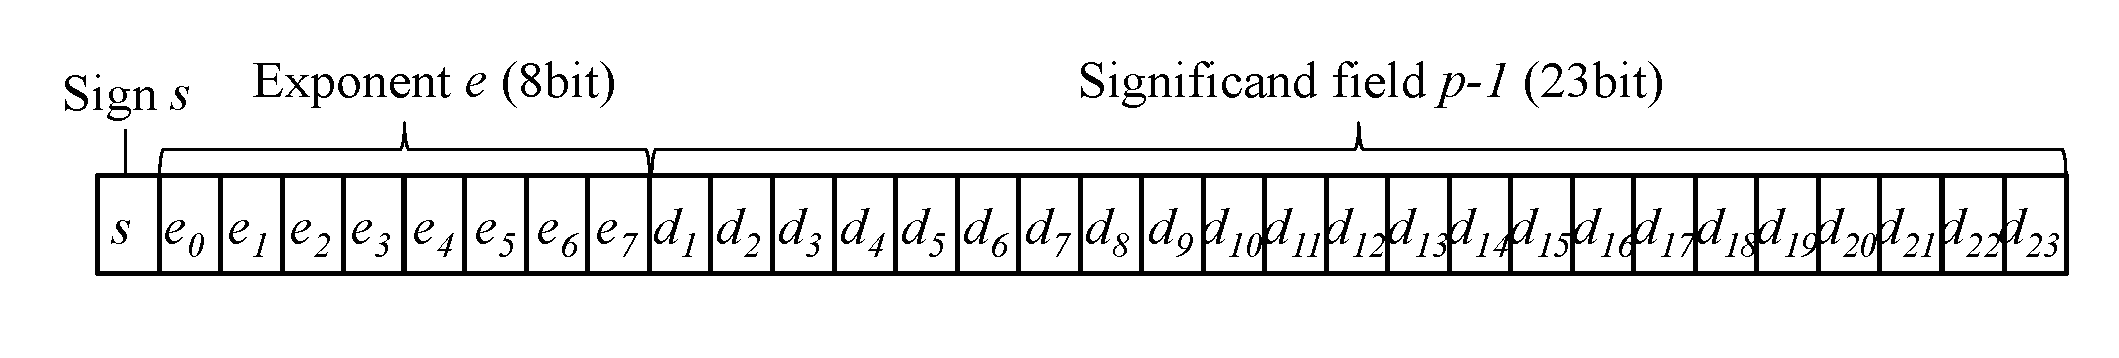
\includegraphics[width=\linewidth]{figs/3_fig_float.eps}
 \end{center}
  \caption{\textit{Single}の場合の表現方法}
 \label{3:fig_float}
\end{figure}

\Mondai
	10進数$7.25$を浮動小数点数に変換せよ．
	ただし，$p$は($d_0$も含め)$6$ bitとし，$e$は$3$ bitとする．\\

\Kaitou
	\begin{align*}
	7.25 &= (111.01)_2 \\
	&= (-1)^0 \times 2^2 \times (1.1101)_2
	\end{align*}
	ここで，$(\cdot)_2$は2進数を意味する．
	そのため，解答は
	\begin{align*}
	0 ~~ 010 ~~ 11010
	\end{align*}
	となる．\\

仮数部$p = 3$ bitとすると，上記の例題にある仮数部のビット$11010$は表現できないことに気が付くと思います．

${\mathbb{F}}$をIEEE 754 規格で定義された浮動小数点数の集合とします．
もちろん，${\mathbb{F}} \subset {\mathbb{R}}$であることに注意してください．
そのとき，IEEE 754 標準における切り捨てや切り上げなどの丸めは，$+ , ~ -, ~ *, ~  /, ~ \sqrt{\cdot} $ の\uwave{5つの演算結果に限り，丸めが定義}されています．
ここで注意点として，入力や出力，初等関数$\sin$などの丸めに関しては定義されていないので注意してください．
実際に，$\circ \in \{ +, -, \times, /  \}$としたとき，以下の例えば3つの丸めモードがあります(ちなみに，2008年に制定されたIEEE 754 規格では全部で5つの丸めモードがあります．):

\begin{enumerate}[label=\alph*), leftmargin=8mm, topsep=2pt, itemsep=0pt, parsep=0pt]
\item 最近点丸め: ~ $\tilde{\circ} : {\mathbb F} \times {\mathbb F} \rightarrow {\mathbb F}$とし，最も近い浮動小数点数に丸める
\item 上向き丸め: ~ $\overline{\circ} : {\mathbb F} \times {\mathbb F} \rightarrow {\mathbb F}$とし，inf$\{x\ \in \ \F\ |\ x \geq a \circ b \}$
\item 下向き丸め: ~ $\underline{\circ} : {\mathbb F} \times {\mathbb F} \rightarrow {\mathbb F}$とし，sup$\{x\ \in \ \F\ |\ x \leq a \circ b\}$
\end{enumerate}

例えば，C99準拠のC言語コンパイラではfenv.hを使用することで，丸めモードの変更を行うfesetround関数が利用できます．
ただし，コンパイラの最適化により計算順序が変更されたり，IEEE 754 標準に準拠しない演算を行われ，意図せずに精度保証付き数値計算として成立しなくなる場合があります．
そのために最適化の抑制として，C言語で定められているvolatile属性を変数に付加することで最適化を抑制したり，浮動小数点数に関する最適化オプション(-fp-modelなど)がコンパイラオプションとしてある場合は最も厳格に準拠(strict)するような設定する必要があります．\\


\Mondai
次のプログラムについて問に答えよ:\\
(1) 誤差が発生する行を答えよ．\\
(2) 丸めモードの変更により動作が保証されている行を答えよ．

\begin{verbatim}
1   #include <stdio.h>
2   #include <math.h>
3	
4   int main(void){
5     double a = 0.1;
6     double b = 1.1;
7     double c;
8
9     c = a + b;
10  
11    printf("%lf\n", c);
12  }
\end{verbatim}

\Kaitou
	(1) 5, 6, 9, 11行目\\
	(2) 9行目(四則演算と平方根のみ丸めモードの変更による動作が保証されている)



%From \ref{3:fig_plus_minus} , the real number $r$ is enclosed by interval [$\bigtriangledown r$,$\bigtriangleup r$].

%\begin{figure}[htb]
% \begin{minipage}{0.4\hsize}
% \begin{center}
%  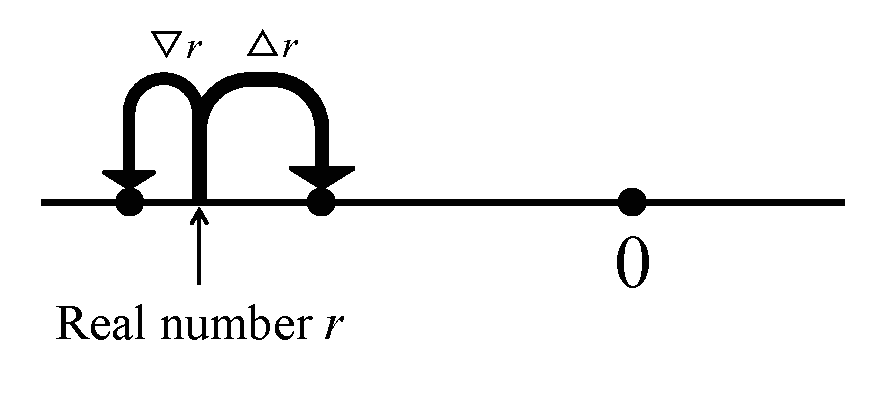
\includegraphics[width=58mm]{figs/3_minus.eps}
% \end{center}
%  \end{minipage}
% \begin{minipage}{0.4\hsize}
% \begin{center}
%  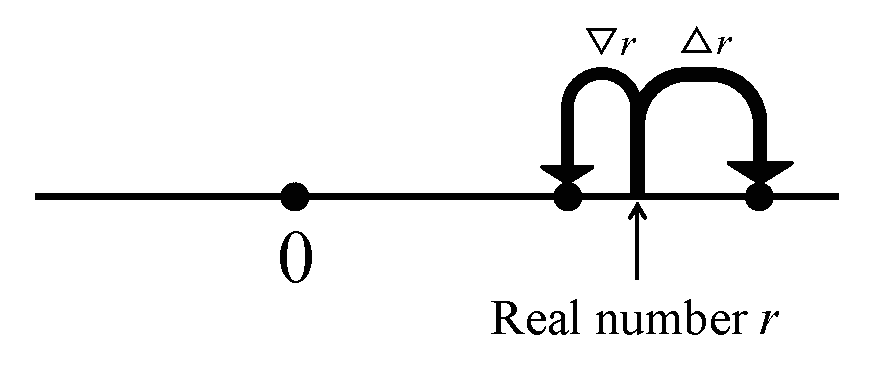
\includegraphics[width=58mm]{figs/3_plus.eps}
% \end{center}
%  \end{minipage}
%   \caption{Rounding ($\cdot$ is a floating-point number).}
% \label{3:fig_plus_minus}
%\end{figure}

%
%----------------------------------------------------------------------------------------------------------------------------------------------
%\subsection{浮動小数点演算の正規化数}

%
%----------------------------------------------------------------------------------------------------------------------------------------------
%\subsection{浮動小数点演算の非正規化数}

%
%----------------------------------------------------------------------------------------------------------------------------------------------
%\subsection{浮動小数点演算のアンダーフローとオーバーフロー}

%
%
%----------------------------------------------------------------------------------------------------------------------------------------------
%----------------------------------------------------------------------------------------------------------------------------------------------
%----------------------------------------------------------------------------------------------------------------------------------------------
\section{1回の浮動小数点数同士の演算における品質保証}
ここでは1回の浮動小数点数同士の演算における結果の品質保証法を紹介します．
具体的には，$a, b \in {\mathbb F}$，すなわち，$a$も$b$も誤差なく浮動小数点数で記述されているとしたときの四則演算($a+b$, $a-b$, $a*b$, $a/b$)の品質保証について取り上げます．

品質の保証を行う際の信念は，「1 bitたりともさぼらずに必ず数学的に正しい結果」を返すことです．
しかしながら，$a+b$という結果は多くの場合，実数${\mathbb R}$になってしまいコンピュータでは表現できません．
そこで，コンピュータで表現できる$a+b$で表せる数学的に正しい結果は，2つの浮動小数点数$c_l, c_u \in {\mathbb F}$を用いて
\begin{align*}
	c_l \le a + b \le c_u
\end{align*}
のように結果を挟み込むことです．
別の言い方をすれば，「区間$[c_l, c_u]$の中に$a + b$の結果が含まれている」あるいは「$a + b \in [c_l, c_u]$」といえます．
もちろん$c_l$と$c_u$の幅が大きければ，使い物にならない結果かもしれません．

では，次に$c_l$と$c_u$をどのように作ればよいか，考えてみましょう．
まず，演算子$+$を用いて丸めも含めた演算をもう一度おさらいすると
\begin{align*}
 a + b \in {\mathbb R}&: ~ \mbox{数学における足し算．結果は浮動小数点数とは限らない} \\
 a ~ \tilde{+} ~ b \in {\mathbb F}&: ~ \mbox{$a+b$に最も近い浮動小数点数．} \\
 a ~ \overline{+} ~ b \in {\mathbb F}&: ~ \mbox{$a+b$よりも大きい浮動小数点数のうち最も小さい数．}\\
 a ~ \underline{+} ~ b \in {\mathbb F}&: ~ \mbox{$a+b$よりも小さい浮動小数点数のうち最も大きい数．}
\end{align*}
でした．
IEEE 754 標準では，$+$以外にも$-, *, /$と$\sqrt{\cdot}$のみ丸めモードの変更による動作の保証がされておりましたね．
よって，$c_l = a ~ \underline{+} ~ b$, $c_u = a ~ \overline{+} ~ b$とすれば，
\begin{align*}
	a + b \in [ a ~ \underline{+} ~ b, a ~ \overline{+} ~ b  ] = \{ c \in {\mathbb R} ~ | ~  a ~ \underline{+} ~ b \le c \le a ~ \overline{+} ~ b \}
\end{align*}
となり，$a + b$の真の結果はわからないですが，コンピュータで数学的に正しい結果$[ a ~ \underline{+} ~ b, a ~ \overline{+} ~ b  ]$を得ることができます．

同様に他の四則演算についても
\begin{align*}
	a - b &\in [ a ~ \underline{-} ~ b, a ~ \overline{-} ~ b  ] \\
	a \cdot b &\in [ a ~ \underline{\cdot} ~ b, a ~ \overline{\cdot} ~ b  ] \\
	a / b &\in [ a ~ \underline{/} ~ b, a ~ \overline{/} ~ b  ]
\end{align*}
のように2つの浮動小数点数の丸めモードを用いて真の結果を含む区間を得ることができます．

\Mondai
プログラム
\begin{verbatim}
   #include <stdio.h>
   #include <math.h>
	
   int main(void){
     double a = 0.1;
     double b = 1.1;
     double c;

     c = a + b;
  
     printf("%lf\n", c);
   }
\end{verbatim}
の$a$と$b$を品質保証を行う計算に変えよ($c$については次節で取り扱う)．
ただし，丸めモードは以下のような fenv.h を使用すること:
\begin{verbatim}
	#include <fenv.h>
	#include <math.h>

	fesetround(FE_UPWARD);    // 上向き丸めモードへ変更
	fesetround(FE_DOWNWARD);  // 下向き丸めモードへ変更
	fesetround(FE_TONEAREST); // 最近点丸めモードへ変更
\end{verbatim}

\vspace{5mm}

\Kaitourei
$0.1$と書いてしまうと誤差が発生するために，$1.0/10.0$のように倍精度浮動小数点数で誤差なく記述できる値の計算に変形してから，丸めモードを用いて上端と下端を計算すればよい ($1.1$についても同様である)．
具体的には以下のようなプログラムになる．
\begin{verbatim}
   #include <stdio.h>
   #include <fenv.h>
   #include <math.h>
	
   int main(void){

     fesetround(FE_DOWNWARD);
       double al = 1.0/10.0;    // 下向き丸めで1/10を計算
     fesetround(FE_UPWARD);
       double au = 1.0/10.0;    // 上向き丸めで1/10を計算

     fesetround(FE_DOWNWARD);
       double bl = 11.0/10.0;    // 下向き丸めで11/10を計算
     fesetround(FE_UPWARD);
       double bu = 11.0/10.0;    // 上向き丸めで11/10を計算

     double c;
     c = a + b;  // ここはどうする?っていうのが次の話!

     printf("%lf\n", c);
   }
\end{verbatim}



上記の解答を見てみると，それぞれ$0.1 \in [a_l, a_u]$, $1.1 \in [b_l, b_u]$となる区間が得られます．
ただし，よく見ると同じ計算(例えば$1.0/10.0$)が出てきます．
もちろん，丸めモードを変えているので，結果は変わります．
しかし，プログラムにはコンパイラの最適化オプションによっては，賢いコンパイラによって$1.0/10.0$は同じ計算だとみなされてしまい
\begin{verbatim}
     fesetround(FE_DOWNWARD);
       double al = 1.0/10.0;    // 下向き丸めで1/10を計算
     fesetround(FE_UPWARD);
       double au = al;

     fesetround(FE_DOWNWARD);
       double bl = 11.0/10.0;    // 下向き丸めで11/10を計算
     fesetround(FE_UPWARD);
       double bu = bl;
\end{verbatim}
のように意図とは違うプログラムに置き換えてしまうかもしれませんので，注意してください．


%
%----------------------------------------------------------------------------------------------------------------------------------------------
%----------------------------------------------------------------------------------------------------------------------------------------------
%----------------------------------------------------------------------------------------------------------------------------------------------
\section{上端下端型の区間演算} \label{intval}
前節の問題の解答例では,$a = 0.1 \in[a_l, a_u]$, $b = 1.1 \in [b_l, b_u]$のように端点が浮動小数点数となる区間を用いて，$0.1$や$1.1$をコンピュータで数学的に正しく保持しました．
しかし，その先のプログラムでは$c = a + b$を計算しています．
このままでは，区間同士の$+$の意味や規則がわからないため，コンパイルエラーになってしまいます．
本節では，区間同士の四則演算を定義することで，演算結果の品質を保証することが目標です．

まず，丸め誤差が入らない状況における区間同士の演算を考えています．
$a \in[a_l, a_u]$, $b \in [b_l, b_u]$としたときの$a + b$の結果は集合
\begin{align*}
	\{ a + b \in {\mathbb R} ~ | ~ \forall a \in [a_l, a_u], ~ \forall b \in [b_l, b_u] \}
\end{align*}
で表されます．
もちろん足し算以外の四則演算($-, \cdot, /$)でも同じです．
例えば，$a = 0.1 \in[a_l, a_u]$, $b = 1.1 \in [b_l, b_u]$のとき，$a + b = 1.2$は
\begin{align*}
	1.2 \in \{ a + b \in {\mathbb R} ~ | ~ \forall a \in [a_l, a_u], ~ \forall b \in [b_l, b_u] \}
\end{align*}
のように集合内に元の足し算結果が必ず含まれます．
すなわち，この右辺の集合を区間同士の演算結果として考えれば，数学的に正しい結果を得ることが可能です．
すなわち，区間同士の四則演算は
\begin{align*}
	[a_l, a_u] + [b_l, b_u] =& \{ a + b \in {\mathbb R} ~ | ~  \forall a \in [a_l, a_u], ~ \forall b \in [b_l, b_u]  \} \\
	[a_l, a_u] - [b_l, b_u] =& \{ a - b \in {\mathbb R} ~ | ~  \forall a \in [a_l, a_u], ~ \forall b \in [b_l, b_u]  \} \\
	[a_l, a_u] \cdot [b_l, b_u] =& \{ a \cdot b \in {\mathbb R} ~ | ~  \forall a \in [a_l, a_u], ~ \forall b \in [b_l, b_u]  \} \\
	[a_l, a_u] / [b_l, b_u] =& \{ a / b \in {\mathbb R} ~ | ~  \forall a \in [a_l, a_u], ~ \forall b \in [b_l, b_u]  \}
\end{align*}
のように定義します．
そのうえで，右辺の集合は閉区間になり，端点$a_l, a_u, b_l, b_u \in {\mathbb R}$のみで書き表せることが知られています:
\begin{itemize}
	\item 加算：$ \{ a + b ~ | ~a \in [a_l, a_u], b \in [b_l, b_u] \} = [a_l + b_l, \ a_u + b_u]$
	\item 減算：$ \{ a - b ~ | ~a \in [a_l, a_u], b \in [b_l, b_u] \} = [a_l - b_u,\ a_u - b_l]$
	
	\item 乗算：$ \{ a \cdot b ~ | ~a \in [a_l, a_u], b \in [b_l, b_u] \} = $\\
	$ ~~~~~~~~~ [\min \{ a_l \cdot b_l, ~ a_u \cdot b_l, ~ a_l \cdot b_u, ~ a_u \cdot b_u \}, ~ \max \{ a_l \cdot b_l, ~ a_u \cdot b_l, ~ a_l \cdot b_u, ~ a_u \cdot b_u \} ]$
	\item 除算：$ \{ a / b ~ | ~a \in [a_l, a_u], b \in [b_l, b_u] \} = $\\
	$ ~~~~~~~~~ [\min \{ a_l / b_l, ~ a_u / b_l, ~ a_l / b_u, ~ a_u / b_u \}, ~ \max \{ a_l / b_l, ~ a_u / b_l, ~ a_l / b_u, ~ a_u / b_u \} ]$\\
	$ ~~~~~~~~~ $ただし$0 \notin [b_l,\ b_u]$
\end{itemize}
この演算で計算した区間の中には，真の答えが必ず含まれています．




しかし，この区間の端点も浮動小数点数で表さなければコンピュータで取り扱うことができません．
注意していただきたい点は，端点$a_l, a_u, b_l, b_u$は，既に浮動小数点数として計算機で保持できていることが前提です．
演算前の端点$a_l, a_u, b_l, b_u$が浮動小数点数でない場合，演算以前に品質保証の取り扱いにミスがあるので注意してください．
ここで気にしなければならない誤差は，演算結果を構成する端点$a_l, a_u, b_l, b_u \in {\mathbb F}$同士の演算(例えば，$a_l + b_l$など)の誤差です．
例えば，$a_l, a_u, b_l, b_u \in {\mathbb F}$における足し算では
\begin{align*}
	[a_l, a_u] + [b_l, b_u] = [a_l + b_l, \ a_u + b_u] \subset& [a_l ~ \underline{+} ~ b_l, \ a_u ~ \overline{+} ~ b_u]
\end{align*}
のように，丸めモードの変更を変更することで，真の像を包含するような区間を作成します．
ここでは，丸めモードまで含めた演算規則として，以下のような機械区間演算を定義します:

\begin{defi}[機械区間演算]\label{def:round_interval}
$a_l, a_u, b_l, b_u \in {\mathbb F}$としたとき，以下として機械区間演算を定義する:
\begin{itemize}
	\item 加算：$[a_l,\ a_u]+[b_l,\ b_u] = [a_l ~ \underline{+} ~ b_l,\ a_u ~ \overline{+} ~ b_u]$
	\item 減算：$[a_l,\ a_u]-[b_l,\ b_u] = [a_l ~ \underline{-} ~ b_u,\ a_u ~ \overline{-} ~ b_l]$
	
	\item 乗算：$ [a_l,\ a_u]\times[b_l,\ b_u] = $\\
	$ ~~~~~~~~~ [\min \{ a_l ~ \underline{\cdot} ~ b_l, a_u ~ \underline{\cdot} ~ b_l, a_l ~ \underline{\cdot} ~ b_u,\ a_u ~ \underline{\cdot} ~ b_u \}, \max \{ a_l ~ \overline{\cdot} ~ b_l, a_u ~ \overline{\cdot} ~ b_l, a_l ~ \overline{\cdot} ~ b_u, a_u ~ \overline{\cdot} ~ b_u \}]$
	\item 除算：$ [a_l,\ a_u]/[b_l,\ b_u]= $\\
	$ ~~~~~~~~~ [\min \{ a_l ~ \underline{/} ~ b_l, a_u ~ \underline{/} ~ b_l, a_l ~ \underline{/} ~ b_u,\ a_u ~ \underline{/} ~ b_u \}, \max \{ a_l ~ \overline{/} ~ b_l, a_u ~ \overline{/} ~ b_l, a_l ~ \overline{/} ~ b_u, a_u ~ \overline{/} ~ b_u \}]$\\
	$ ~~~~~~~~~ $ただし$0 \notin [b_l,\ b_u]$
\end{itemize}
\end{defi}

\Mondai
プログラム
\begin{verbatim}
   #include <stdio.h>
   #include <math.h>
	
   int main(void){
     double a = 0.1;
     double b = 1.1;
     double c;

     c = a + b;
  
     printf("%lf\n", c);
   }
\end{verbatim}
の$a$と$b$及び，$c = a + b$の品質保証を行う計算に変えよ．
ただし，丸めモードは以下のような fenv.h を使用すること:
\begin{verbatim}
	#include <fenv.h>

	fesetround(FE_UPWARD);    // 上向き丸めモードへ変更
	fesetround(FE_DOWNWARD);  // 下向き丸めモードへ変更
	fesetround(FE_TONEAREST); // 最近点丸めモードへ変更
\end{verbatim}

\vspace{5mm}

\Kaitourei
$a$と$b$の保証については前節に取り上げてあることに注意し解答を示す:
\begin{verbatim}
   #include <stdio.h>
   #include <fenv.h>
   #include <math.h>
	
   int main(void){

     fesetround(FE_DOWNWARD);
       double al = 1.0/10.0;    // 下向き丸めで1/10を計算
     fesetround(FE_UPWARD);
       double au = 1.0/10.0;    // 上向き丸めで1/10を計算

     fesetround(FE_DOWNWARD);
       double bl = 11.0/10.0;    // 下向き丸めで11/10を計算
     fesetround(FE_UPWARD);
       double bu = 11.0/10.0;    // 上向き丸めで11/10を計算

     fesetround(FE_TONEAREST);  // 最近点丸めにもどす

     double cl, cu;
     fesetround(FE_DOWNWARD);
       cl = al + bl;
     fesetround(FE_UPWARD);
       cu = au + bu;

     fesetround(FE_TONEAREST);  // 最近点丸めにもどす

     printf("%lf\n", cl);
     printf("%lf\n", cu);
   }
\end{verbatim}

\vspace{5mm}


以下の問題は，ベクトル，行列を扱う際に良く使う演算です．
場合によっては，計算途中の結果を区間として保持する必要がなく，一気に計算可能な例があります．
どのような演算が一気に計算可能な例になるか覚えておきましょう．

\vspace{5mm}

\Mondai
$a, b, c, c_l, c_u \in {\mathbb F}$とする．
そのとき，以下の結果を包含する両端点に浮動小数点数を持つ区間を，丸めモード変更付きの四則演算を用いて作成せよ:
\begin{align*}
	\mbox{(1)}& ~ a \cdot b - c \\
	\mbox{(2)}& ~c - a \cdot b \\
	\mbox{(3)}& ~a \cdot b + [ c_l, c_u ]
\end{align*}

\vspace{5mm}

\Kaitourei
\noindent\textbf{(1)}:
\begin{align*}
	a \cdot b - c \subset& [ a ~ \underline{\cdot} ~ b, ~ a ~ \overline{\cdot} ~ b  ] - c \\
	=& [ a ~ \underline{\cdot} ~ b, ~ a ~ \overline{\cdot} ~ b  ] - [c, c] \\
	\subset&  [ a ~ \underline{\cdot} ~ b ~ \underline{-} ~ c , ~ a ~ \overline{\cdot} ~ b ~ \overline{-} ~ c  ]
\end{align*}
注意点としては，$[ a ~ \underline{\cdot} ~ b, ~ a ~ \overline{\cdot} ~ b  ] - c$は$[ a ~ \underline{\cdot} ~ b, ~ a ~ \overline{\cdot} ~ b  ] - [c, c]$のように$c$を点区間として計算すればよい．
上記の計算により，
\begin{verbatim}
     fesetround(FE_DOWNWARD);
       res_lower = a*b - c;
     fesetround(FE_UPWARD);
       res_upper = a*b - c;
\end{verbatim}
のように途中結果を区間として保持せずに区間を作成できる．

\medskip\noindent\textbf{(2)}:
\begin{align*}
	c - a \cdot b \subset& c - [ a ~ \underline{\cdot} ~ b, ~ a ~ \overline{\cdot} ~ b  ]  \\
        \subset& [c, c] - [ a ~ \underline{\cdot} ~ b, ~ a ~ \overline{\cdot} ~ b  ]  \\
	\subset&  [ c ~ \underline{-} ~ a ~ \overline{\cdot} ~ b , ~ c ~ \overline{-} ~a ~ \underline{\cdot} ~ b  ]
\end{align*}
上記の計算により，
\begin{verbatim}
     fesetround(FE_DOWNWARD);
       tmp_lower = a*b;
     fesetround(FE_UPWARD);
       tmp_upper = a*b;
       res_upper = c - tmp_lower;
     fesetround(FE_DOWNWARD);
       res_lower = c - tmp_upper;
\end{verbatim}
のように$a \cdot b$の結果を区間として保持しなければならない．

初めて扱った人がしがちなミスとして
\begin{verbatim}
     誤ったプログラム:
     fesetround(FE_DOWNWARD);
       res_lower = c - a*b;
     fesetround(FE_UPWARD);
       res_upper = c - a*b;
\end{verbatim}
としてしまいます．
これでは，数学的に正しくない結果を返しているので注意してください．

\medskip\noindent\textbf{(3)}:
\begin{align*}
	a \cdot b + [ c_l, c_u ] \subset& [ a ~ \underline{\cdot} ~ b, ~ a ~ \overline{\cdot} ~ b  ] + [ c_l, c_u ] \\
	\subset& [ a ~ \underline{\cdot} ~ b ~ \underline{+} ~ c_l , ~ a ~ \overline{\cdot} ~ b ~ \overline{+} ~ c_u  ]
\end{align*}
上記の計算により，
\begin{verbatim}
     fesetround(FE_DOWNWARD);
       res_lower = a*b + cl;
     fesetround(FE_UPWARD);
       res_upper = a*b + cu;
\end{verbatim}
のように$a \cdot b$の結果を保持せずに区間を作成できる．
この結果から浮動小数点数の$n$次元ベクトル$a \in {\mathbb F}^n$と$b \in {\mathbb F}^n$の内積$a \cdot b$は区間
\begin{align}\label{eq:inner_def}
	[ a_1 \underline{\cdot} b_1 \underline{+} a_2 \underline{\cdot} b_2 \underline{+} \cdots \underline{+}  a_n \underline{\cdot} b_n, ~~ a_1 \overline{\cdot} b_1 \overline{+} a_2 \overline{\cdot} b_2 \overline{+} \cdots \overline{+}  a_n \overline{\cdot} b_n ]
\end{align}
として得られるため，
\begin{verbatim}
     fesetround(FE_DOWNWARD);
       for (int i = 0; i < n; i++)
         res_lower += a[i]*b[i];
     fesetround(FE_UPWARD);
       for (int i = 0; i < n; i++)
         res_upper += a[i]*b[i];
\end{verbatim}
のように計算できる．
この例のように「一気に計算する技を利用できるのはあくまで数学的に正しい状況のみ」で，基本は「機械区間演算」であることに注意してください．

%
%----------------------------------------------------------------------------------------------------------------------------------------------
%----------------------------------------------------------------------------------------------------------------------------------------------
%----------------------------------------------------------------------------------------------------------------------------------------------
\section{浮動小数点数で成分を持つ点行列同士の行列積}
前節の\eqref{eq:inner_def}の結果をまとめると浮動小数点数で成分を持つベクトルの内積は次のようなことが言えます:

\begin{Thm}[浮動小数点数における内積の包含] \label{thm:float_inner}
	浮動小数点数の$n$次元のベクトル$a \in {\mathbb F}^n$と$b \in {\mathbb F}^n$は
	\begin{align*}
		a \cdot b \subset [ a ~ \underline{\cdot} ~ b , a ~ \overline{\cdot} ~ b ]
	\end{align*}
	となる．
	ただし，$a \underline{\cdot} b$は内積の演算をすべて下向き丸めで計算し，$a \overline{\cdot} b$は内積の演算をすべて上向き丸めで計算することを意味し，\eqref{eq:inner_def}のように計算していることを前提とする．
\end{Thm}

もちろん，同じように行列積についても以下のことがいえます:
\begin{Thm}[浮動小数点数における行列積の包含] \label{thm:float_matmul}
	浮動小数点数の行列$A \in {\mathbb F}^{l \times m}$と$B \in {\mathbb F}^{m \times n}$は
	\begin{align*}
		A \cdot B \subset [ A ~ \underline{\cdot} ~ B , A ~ \overline{\cdot} ~ B ]
	\end{align*}
	となる．
	ただし，$A \underline{\cdot} B$は行列積の演算をすべて下向き丸めで計算し，$a \overline{\cdot} b$は行列積の演算をすべて上向き丸めで計算することを意味し，各成分ごとで現れる内積は\eqref{eq:inner_def}のように計算していることを前提とする．
\end{Thm}

最後の注意書きは，行列積を工夫するアルゴリズムStrassenなどでは引き算が含まれるため，上記の定理の範囲外になってしまいますので注意してください．
例えば，$A,\ B\in\F^{n\times n}$としたときの行列積は以下のように計算できます:

\begin{verbatim}
	#include <fenv.h>
	fesetround(FE_UPWARD);   //上向き丸めモードへ変更
	C_u=A*B;                 //上向き丸めで行列積
	fesetround(FE_DOWNWARD); //下向き丸めモードへ変更
	C_d=A*B;                 //下向き丸めで行列積
\end{verbatim}

行列積$A*B$に最適化されたBLAS(例えばdgemmなど)を用いることで非常に高速に点行列同士の積の包含を得ることができます．
ただし，例えば3つの行列の積$A*B*C$などの一般的な場合は区間行列の演算になるため結果の包含は単純には得られないので注意してください．
区間同士の行列積については\ref{chap:basic_matrix}章で取り上げます．

また，注意点としては，$A*B$を演算する前に丸めモードを変更していますが，行列演算に利用する全ノード・全スレッドの丸めモードが変更されている必要があります．
そのため，BLASなどの高速ルーチンを利用する際には全ノード・全スレッドの丸めモードが変更されている保証が必要になります．


%
%----------------------------------------------------------------------------------------------------------------------------------------------
%----------------------------------------------------------------------------------------------------------------------------------------------
%----------------------------------------------------------------------------------------------------------------------------------------------
\section{区間演算の落とし穴}
区間演算を初めて勉強したとき著者は「すべて区間演算で計算すればいいんじゃない?」って思いました．
しかし，残念ながら世の中そんなにうまい話はなく，「区間演算を繰り返すことによる過大評価」という最大の欠点があります．
そのために，現在では，「最初に近似解を求めてから，その結果の品質を保証する際に区間演算を使う」という検算手法として区間演算は利用されます．
連立一次方程式を例にとると，(1) Gaussの消去法は通常の浮動小数点数の演算で行い近似解を得る，(2) そのうえで，得られた近似解と真の解の誤差を計算する際に区間演算で数学的に正しい結果で証明，のような流れです．

ここでは，欠点となる例をいくつか紹介したいと思います．
まず，$x^2, x \in [-1, 1]$について取り扱いたいと思います．
$x^2 = x \cdot x$だからといって演算を行うと
\begin{align*}
	[-1, 1] \cdot [-1, 1] = [-1, 1]
\end{align*}
となります．
もちろん，この結果は数学的には正しいです．
しかし，よく考えると$0 \le x^2, \forall x \in {\mathbb R}$ですので，負の値が区間に含まれてしまう結果は良い結果とは言えません．
この原因は，区間演算の定義に立ち戻ると
\begin{align*}
	[-1, 1] \cdot [-1, 1] = \{ x \cdot y ~ | ~ x \in [-1, 1], ~ y \in [-1, 1]  \}
\end{align*}
となり，$x$と$y$は独立した変数としてみなしているため$x = 1, y = -1$のような状況が発生し，負の値が生まれます．
本来は$x^2$の像は
\begin{align*}
	[-1, 1]^2 = \{ x^2 = x \cdot x ~ | ~ x \in [-1, 1]  \}
\end{align*}
となるため，$x \cdot y$のように独立には動かず
\begin{align*}
	[-1, 1]^2 = [0, 1]
\end{align*}
のようになります．
あくまで区間演算は2つの区間に依存関係がない独立した変数としての結果となるため，依存関係がある演算を行う場合には過大評価になってしまいます．

同じように，$x \in [-1, 1]$に対して，
\begin{align*}
	x - x = [-1, 1] - [-1, 1] = [-2, 2] = \{ x - y ~ | ~ \forall x \in [-1, 1], ~ \forall y \in [-1, 1]  \}
\end{align*}
となってしまうため，過大評価になってしまいます(実際は$\{ x - x = 0 ~ | ~ \forall x \in [-1, 1]  \}$)．
$x^2$や$x - x$のようにわかりきった計算の場合は，専用の演算をプログラムすればよいですが，例えば漸化式
\begin{align*}
	x_0 \in& [ x_l, x_u ] \\
	x_1 \in& [ y_l, y_u ] \\
	x_{n} =& f(x_{n-1}, x_{n - 2})
\end{align*}
のように依存関係がわかりにくくなってしまう演算は非常に多くあります．
解消法としては，平均値形式やアフィン演算などがありますが，本書では取り扱いません．


次の例として回転行列
\begin{align*}
	A(\theta) = \left( \begin{array}{cc}
	\cos(\theta) & -\sin(\theta) \\
	\sin(\theta) & \cos(\theta)
	\end{array}\right),
\end{align*}
と区間ベクトル
\begin{align*}
	x = \left( \begin{array}{c}
	x_1 \\
	x_2
	\end{array}\right) = \left(
	\begin{array}{c}
	\mbox{[-1, 1]} \\
	\mbox{[-1, 1]}
	\end{array}
	\right).
\end{align*}
について考えてみます．
$x$を図で書いてみると図 \ref{3:wrap1}のようになります．

\begin{figure}[htb]
 \begin{center}
  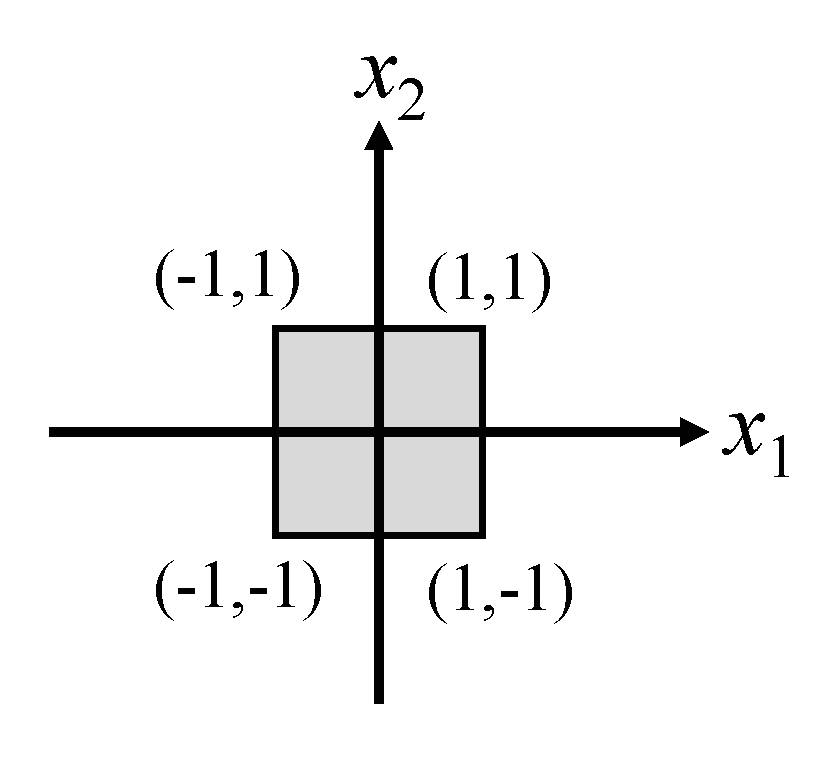
\includegraphics[width=50mm]{figs/wrapping_effect1.eps}
 \end{center}
  \caption{Wrapping effect1}
 \label{3:wrap1}
\end{figure}

$\pi/4$だけ$x$を回転を意味する$A(\pi/4)x$の像は図 \ref{3:wrap2}のようになります．
しかしながら，区間演算を用いて計算すると
\begin{align*}
	A(\pi/4)x = \left( \begin{array}{cc}
	\frac{\sqrt{2}}{2} & -\frac{\sqrt{2} }{2} \\
	\frac{\sqrt{2} }{2} & \frac{\sqrt{2} }{2}
	\end{array}\right)\left(
	\begin{array}{c}
	\mbox{[-1, 1]} \\
	\mbox{[-1, 1]}
	\end{array}
	\right) = \left(
	\begin{array}{c}
	\mbox{[}-\sqrt{2}, \sqrt{2}\mbox{]} \\
	\mbox{[}-\sqrt{2}, \sqrt{2}\mbox{]}
	\end{array}
	\right),
\end{align*}
のようになり，図で表すと図 \ref{3:wrap3}のオレンジ色の部分になります．
図を見てもわかるように，区間演算はそれぞれの軸に対して区間を作成するために，2次元ベクトル以上の場合は表現できる集合が非常に限定されてしまいます．

\begin{figure}[htb]
 \begin{center}
  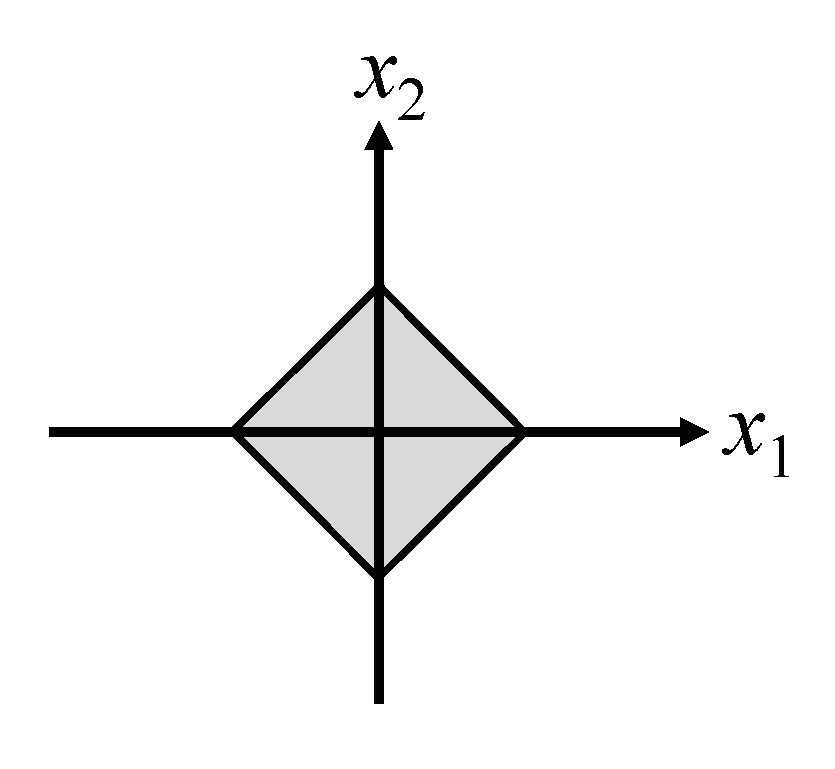
\includegraphics[width=50mm]{figs/wrapping_effect2.eps}
 \end{center}
  \caption{Wrapping effect2}
 \label{3:wrap2}
\end{figure}

\begin{figure}[htb]
 \begin{center}
  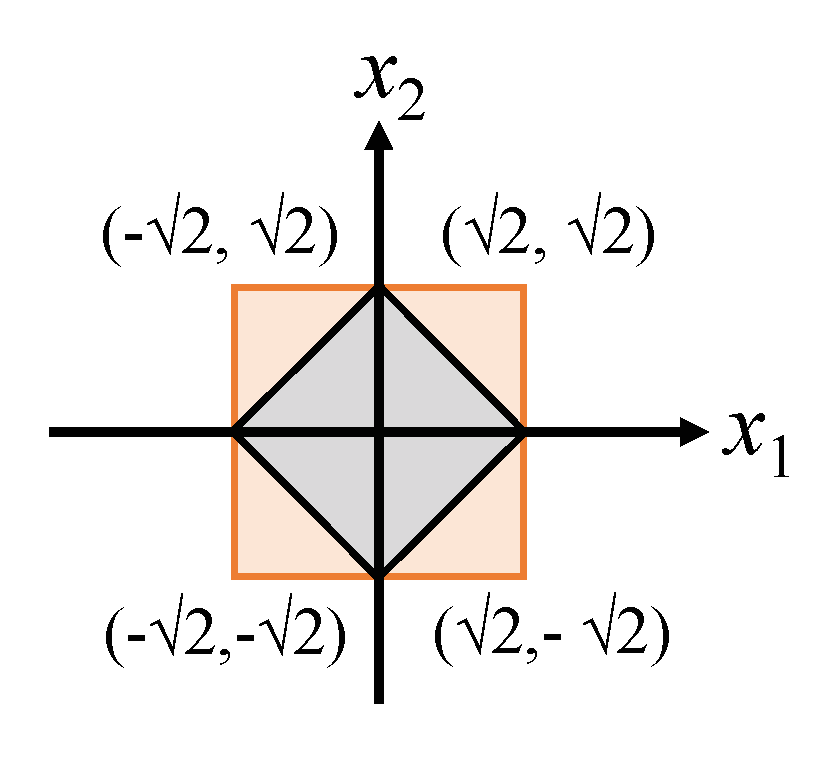
\includegraphics[width=50mm]{figs/wrapping_effect3.eps}
 \end{center}
  \caption{Wrapping effect3}
 \label{3:wrap3}
\end{figure}

さらに，もう一度，$\pi/4$だけ回転させる，すなわち$A(\pi/4) \left( A(\pi/4)x \right)$とすると真の像は図 \ref{3:wrap2}に戻ります．
しかしながら，区間演算では
\begin{align*}
A\left( \frac{\pi}{4} \right) \left( A\left( \frac{\pi}{4} \right)x \right) = \left(
\begin{array}{c}
\mbox{[}-2, 2\mbox{]} \\
\mbox{[}-2, 2\mbox{]}
\end{array}
\right)
\end{align*}
から図 \ref{3:wrap4}のようになり，非常に過大評価になってしまうことがわかります．

\begin{figure}[htb]
 \begin{center}
  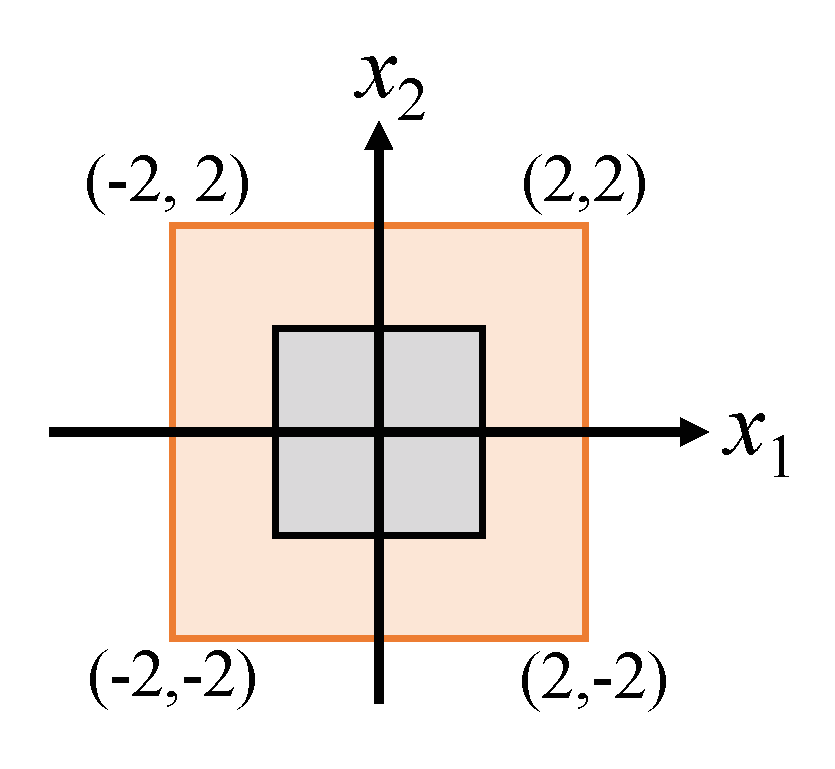
\includegraphics[width=50mm]{figs/wrapping_effect4.eps}
 \end{center}
  \caption{Wrapping effect4}
 \label{3:wrap4}
\end{figure}

このような影響はラッピングエフェクトと呼ばれます．
そのために，区間演算はできる限り後に行ったほうがよいです．
例えば，計算順序をかえると
\begin{align*}
\left( A\left( \frac{\pi}{4} \right) A\left( \frac{\pi}{4} \right) \right) x  = \left( \begin{array}{cc}
0 & -1 \\
1 & 0
\end{array}\right)\left(
\begin{array}{c}
\mbox{[-1, 1]} \\
\mbox{[-1, 1]}
\end{array}
\right) = \left(
\begin{array}{c}
\mbox{[}-1, 1 \mbox{]} \\
\mbox{[}-1, 1 \mbox{]}
\end{array}
\right).
\end{align*}
となることから，精度の良い結果を得ることができます．



%
%----------------------------------------------------------------------------------------------------------------------------------------------
%----------------------------------------------------------------------------------------------------------------------------------------------
%----------------------------------------------------------------------------------------------------------------------------------------------
\section{中心半径型の区間と区間演算}\label{sec:midrad_op}
今まで扱ってきた区間$[a_l, a_u] = \{ a \in {\mathbb R} ~ | ~ a_l \le a \le a_u \}$は，上端と下端から表現される区間であるため，ここでは上端下端型の区間と呼びます．
それに対し，中心$a_m \in {\mathbb R}$と半径$a_r \ge 0$を用いても区間
\begin{align*}
	\langle a_m, a_r  \rangle := \{ a \in {\mathbb R} ~ | ~ | a - a_m | \le a_r  \}
\end{align*}
を表現することができ，こちらを中心半径型の区間と呼びます．
本節の目標は，中心半径型の区間を利用することで，過大評価にはなるかわりに最大値/最小値の判別が必要ない計算方法を紹介します．
この方法を拡張することで，区間同士の行列積に適用することができます．
そのうえ，行列積に対し，BLASなどの既存の高速に最適化されたプログラムを利用した高速な品質保証法を実現できます．


まず，上端下端型の区間と中心半径型の区間の関係性は
\begin{align*}
	[ a_l, a_u ] = \left\langle \frac{ a_l + a_u }{2}, ~ \frac{ a_u - a_l }{2}  \right\rangle
\end{align*}
であり，
\begin{align*}
	\langle a_m, a_r  \rangle = [ a_m - a_r, ~ a_m + a_r ]
\end{align*}
となります．
しかしながら，浮動小数点数同士の演算は一般的には浮動小数点数になるとは限らないため，「上端下端型から中心半径型への変換」および「中心半径型から上端下端型への変換」をコンピュータで行う際には誤差が生じます．
そのために，双方の変換でも丸めモードの変更を行い元の区間を包含する区間を作成します．

まず，「コンピュータを用いた中心半径型から上端下端型への変換」は単純であり，$a_m, a_r \in {\mathbb F}$とすると
\begin{align*}
	\langle a_m, a_r  \rangle \subset [ a_m ~ \underline{-} ~ a_r, ~ a_m ~  \overline{+} ~ a_r ]
\end{align*}
として変換することができます．
それに対し，「コンピュータを用いた上端下端型から中心半径型への変換」は中心の演算に対し，どうすれば良いか考えなければなりません．


\begin{Thm}[上端下端型から中心半径型への変換]\label{thm:infsup_to_midrad}
	${\mathbb F}$を基数$2$の浮動小数点数とし，$a_l, a_u \in {\mathbb F}$が$a_l \le a_u$を満たすとする．	  
	そのとき，$a_m, a_r \in {\mathbb F}$を
	\begin{align*}
		a_m = (a_l ~ \overline{+} ~ a_u) \overline{/} 2 , ~ a_r = a_m ~ \overline{-} ~ a_l
	\end{align*}
	とすると，
	\begin{align*}
		[ a_l, a_u ] \subset \langle a_m, a_r \rangle
	\end{align*}
	となる．
\end{Thm}

\begin{Proof}
	$a_m - a_r \le a_l$と$a_u \le a_m + a_r$を示せばよい．

	まず，$a_m - a_r \le a_l$から示す．
	丸めモードの定義から$a_m ~ \overline{-} ~ a_l \ge a_m - a_l$となることに注意すると
	\begin{align*}
		a_l + a_r =a_l + (  a_m ~ \overline{-} ~ a_l ) \ge a_l + (  a_m - a_l ) = a_m
	\end{align*}
	となる．
	よって，上式から$a_r$を引くと$a_l \ge a_m - a_r$になる．

	次に，$a_u \le a_m + a_r$を示す．
	まず，$a_l ~ \overline{+} ~ a_u$の結果は基数$2$の浮動小数点数になる．
	そのうえで，基数$2$の浮動小数点数に対し，(どのような丸めモードでも)$2$を割っても誤差は生じないため，
	\begin{align*}
		(a_l ~ \overline{+} ~ a_u) \overline{/} 2 = (a_l ~ \overline{+} ~ a_u)/2
	\end{align*}
	となる．
	そのうえで，丸めモードの定義から$a_l ~ \overline{+} ~ a_u \ge a_l + a_u$となることに注意すると
	\begin{align*}
		a_m + a_r =& ( (a_l ~ \overline{+} ~ a_u) \overline{/} 2 ) + (a_m ~ \overline{-} ~ a_l) = \left( \frac{a_l ~ \overline{+} ~ a_u}{2} \right) + (a_m ~ \overline{-} ~ a_l) \\
		\ge& \frac{a_l + a_u}{2} + a_m - a_l = \frac{a_l + a_u}{2}  + \left( ( (a_l ~ \overline{+} ~ a_u) \overline{/} 2 \right) - a_l \\
		\ge& \frac{a_l + a_u}{2}  +  \frac{a_l + a_u}{2} - a_l = a_l + a_u - a_l = a_u
	\end{align*}

\qed
\end{Proof}

次に，中心半径型における演算規則を紹介します．
足し算と引き算は
\begin{align*}
	\langle a_m, a_r  \rangle \pm \langle b_m, b_r  \rangle =& [ a_m - a_r, ~ a_m + a_r ] \pm [ b_m - b_r, ~ b_m + b_r ] \\
	=& [a_m \pm b_m - a_r - b_r, ~ a_m \pm b_m + a_r + b_r] \\
	=&  \left\langle a_m \pm b_m, ~ a_r + b_r  \right\rangle
\end{align*}
と簡単に得られます(が，わざわざ中心半径型で行うメリットはありません...)．

それに対し，掛け算は工夫が必要であり，中心半径型で計算するメリット(とデメリット)があります．

\begin{Thm}[中心半径型の区間の積] \label{thm:midrad_mul}
	$a_m,  b_m \in {\mathbb R}$と非負の実数$a_r, b_r \in {\mathbb R}$とする．	  
	そのとき，中心半径型の区間の積は
	\begin{align*}
		\langle a_m, a_r \rangle \cdot \langle b_m, b_r \rangle \subset& \langle a_m \cdot b_m, ~ | a_m | \cdot b_r + a_r \cdot | b_m | + a_r \cdot b_r \rangle
	\end{align*}
	のように評価できる．
\end{Thm}

\begin{Proof}
	$\langle a_m, a_r \rangle$と$\langle b_m, b_r \rangle$を上端下端型で表すと
	\begin{align*}
		\langle a_m, a_r \rangle =& [ a_m - a_r, a_m + a_r ] \\
		\langle b_m, b_r \rangle =& [ b_m - b_r, b_m + b_r ]
	\end{align*}
	となる．
	そのうえ，
	\begin{align*}
		\langle a_m, a_r \rangle \cdot \langle b_m, b_r \rangle =& [ a_m - a_r, a_m + a_r ] \cdot [ b_m - b_r, b_m + b_r ]
	\end{align*}
	となるため，
	\begin{align*}
		(a_m - a_r) ( b_m - b_r ) =& a_m b_m - a_m b_r - a_r b_m + a_r b_r \\
		(a_m - a_r) ( b_m + b_r ) =& a_m b_m + a_m b_r - a_r b_m - a_r b_r \\
		(a_m + a_r) ( b_m - b_r ) =& a_m b_m - a_m b_r + a_r b_m - a_r b_r \\
		(a_m + a_r) ( b_m + b_r ) =& a_m b_m + a_m b_r + a_r b_m + a_r b_r
	\end{align*}
	の最小値と最大値がわかればよい．
	そのうえで，
	\begin{align*}
		&a_m b_m - | a_m | b_r - a_r | b_m | - a_r b_r \\
		&\le \begin{array}[t]{@{}c@{}}
			a_m b_m - a_m b_r - a_r b_m + a_r b_r \\
			a_m b_m + a_m b_r - a_r b_m - a_r b_r \\
			a_m b_m - a_m b_r + a_r b_m - a_r b_r \\
			a_m b_m + a_m b_r + a_r b_m + a_r b_r
		\end{array} \\
		&\le a_m b_m + | a_m | b_r + a_r | b_m | + a_r b_r
	\end{align*}
	となるため，
	\begin{align*}
		\langle a_m, a_r \rangle \cdot \langle b_m, b_r \rangle \subset& [ a_m b_m - | a_m | b_r - a_r | b_m | - a_r b_r, \\
		& \quad a_m b_m + | a_m | b_r + a_r | b_m | + a_r b_r ] \\
		=& \langle a_m b_m, ~ | a_m | b_r + a_r | b_m | + a_r b_r \rangle
	\end{align*}	

\qed
\end{Proof}

定理\ref{thm:midrad_mul}は過大評価というデメリットはあるかわりに，if文や$\max$, $\min$など分岐を必要せずに計算できることが最大のメリットです．
中心半径型の区間の積でもイコールとなる式も知られていますが，if文や$\max$, $\min$が発生するために，(普通に上端下端型の区間を使えばよいので)あまり利用されません．
そのうえで，分岐を必要としない定理\ref{thm:midrad_mul}は，区間同士の内積，行列-ベクトル積，行列-行列積が，点同士の内積，行列-ベクトル積，行列-行列積に帰着され，BLASなどの既存の最適化されたルーチンを使用することができます．
これにより，行列積の非常に高速な品質保証が可能になります．




%
%----------------------------------------------------------------------------------------------------------------------------------------------
%----------------------------------------------------------------------------------------------------------------------------------------------
%----------------------------------------------------------------------------------------------------------------------------------------------

\chapter{区間ベクトル/行列の演算に対する品質保証法} \label{chap:basic_matrix}


%----------------------------------------------------------------------------------------------------------------------------------------------
\section{記号の準備}\label{sec:linear_notation}
本節で定義する記号は本章以降でも利用しますので，定義を忘れた場合に本節に立ち戻って見直してください．
まずは，よく利用するベクトルおよび行列を定義したいと思います．
$\vector{0} \in {\mathbb R}^n$, $O \in {\mathbb R}^{n \times m}$ ~ $I \in {\mathbb R}^{n \times n}$を
\begin{align*}
	\vector{0} := \left( \begin{array}{c}
		0 \\
		0 \\
		\vdots \\
		0
	\end{array}\right), ~ O := \left( \begin{array}{c c c c}
		0 & 0 & \cdots & 0 \\
		0 & 0 & \cdots & 0 \\
		\vdots & \vdots & \ddots & \vdots  \\
		0 & 0 & \cdots & 0
	\end{array}\right), ~ I := \left( \begin{array}{c c c c}
		1 & 0 & \cdots & 0 \\
		0 & 1 & \cdots & 0 \\
		\vdots & \vdots & \ddots & \vdots  \\
		0 & 0 & \cdots & 1
	\end{array}\right)
\end{align*}
のように，それぞれゼロベクトル，ゼロ行列，単位行列とします．


次に，ベクトルおよび行列の半順序($\le$)を定義したいと思います．
2つのベクトル$a = (a_i),  b = (b_i) \in {\mathbb R}^n$あるいは2つの行列$A = (A_{ij}), B = (B_{ij}) \in {\mathbb R}^{n \times m}$に対し，
\begin{align*}
	& a \le b ~ \mbox{はすべての} ~ i ~{について} ~ a_i \le b_i ~ \mbox{が成立} \\
	& A \le B ~ \mbox{はすべての} ~ i, j ~{について} ~ A_{ij} \le B_{ij} ~ \mbox{が成立}
\end{align*}
とします．
すなわち，本書ではベクトル・行列の順序を「各成分で比較し，すべての成分で同じ不等号が成立しているとき」を意味します．

続いて，ベクトルおよび行列の絶対値を定義します．
ベクトル$a = (a_i) \in {\mathbb R}^n$および行列$A = (A_{ij}) \in {\mathbb R}^{n \times m}$に対する絶対値は
\begin{align*}
	| a | := ( | a_i | ) \in {\mathbb R}^{n} , ~~ | A | := ( | A_{ij} | ) \in {\mathbb R}^{n \times m}
\end{align*}
とします．
すなわち，各成分に絶対値をつけたベクトル/行列を意味しています．
特に，$|A|$は行列式ではないのでご注意ください．
もちろん，$| a | \ge \vector{0}$および$| A | \ge O$が成立します．


また，ついでにノルムについても定義をしたいと思います．
抽象的なノルムについては\ref{sec:Banach_space}節の定義\ref{def:App:norm}で記載するとし，ひとまず，記号としてベクトル$x = (x_1, x_2, \cdots x_n)^T \in {\mathbb C}^n$に対する1ノルム，2ノルム，最大値ノルムをそれぞれ
\begin{align*}
	\|x\|_{1} :=  \sum_{i = 1}^n |x_i |, ~~
	\|x\|_{2}\ :=  \sqrt{ \sum_{i = 1}^n |x_i|^2 }, ~~
	\|x\|_{\infty} :=  \mymax_{1\leq i \leq n} |x_i| 
\end{align*}
と定義します．
次に，正方行列$A \in {\mathbb C}^{n \times n}$に固有値を$\lambda_i$としたとき，スペクトル半径$\rho(A)$を
\begin{align*}
	\rho(A) := \mymax_{i} | \lambda_i |
\end{align*}
とします．
また，$A = (a_{ij}) \in {\mathbb C}^{n \times m}$に対する行列のノルムを
\begin{align*}
	\|A\|_{1} :=& \mymax_{1\leq j \leq m}\sum_{i=1}^n|a_{ij}| \\
	\|A\|_{2} :=& \sqrt{ \rho(A^T A) } \\
	\|A\|_{\infty} :=& \mymax_{1\leq i \leq n}\sum_{j=1}^m|a_{ij}|
\end{align*}
と定義します．
行列のノルムについても詳細を知りたい場合，\ref{sec:DX_bounded_linear_op}項の抽象的な線形作用素ノルムに関する定理\ref{thm:set_bound_linear_operator}などを参照してください．

また，区間ベクトルおよび区間行列を
\begin{align*}
	[a, b] :=& \{ c \in {\mathbb R}^n ~ | ~ a \le c \le b, ~ \forall a, b \in {\mathbb R}^n \} \\
	[A, B] :=& \{ C \in {\mathbb R}^{n \times m} ~ | ~ A \le C \le B, ~ \forall A, B \in {\mathbb R}^{n \times m} \}
\end{align*}
とします．
同じように中心半径型の区間ベクトルおよび区間行列も
\begin{align*}
	\langle  c , ~ r \rangle :=& \{ a \in {\mathbb R}^n ~ | ~  | c - a | \le r \in {\mathbb R}^n \} \\
	\langle  C , ~ R \rangle :=& \{ A \in {\mathbb R}^{n \times m } ~ | ~  | C - A | \le R \in {\mathbb R}^{n \times m } \}
\end{align*}
のように定義します．
ここで，$| c - a | \le r $や$| C - A | \le R$はベクトルや行列の絶対値や不等号であることに注意してください．
上端下端型の区間と中心半径型の区間の関係性は，\ref{sec:midrad_op}節と変わらず，
\begin{align*}
	[a, b] =& \langle  (a + b)/2 , ~ (b - a)/2 \rangle,& ~ [A, B] =& \langle  (A + B)/2 , ~ (B - A)/2 \rangle \\
	\langle c, r \rangle =& [ c -r, c + r ] ,& ~ \langle C, R \rangle =& [ C - R, C + R ]
\end{align*}
のようになります．




%
%----------------------------------------------------------------------------------------------------------------------------------------------
%----------------------------------------------------------------------------------------------------------------------------------------------
%----------------------------------------------------------------------------------------------------------------------------------------------
\section{区間行列積の計算方法}
ここでは，区間行列積の計算方法を紹介します．
とはいっても，区間行列積の各成分の結果は，区間ベクトルの内積に帰着されるために，まずは，区間ベクトルの内積にたいする計算方法を紹介します．

まずは，2つの中心半径型の2次元区間ベクトルの内積を考えてみます．
すなわち，$a_m = (a_m^{i}), b_c = (b_m^{i}) \in {\mathbb R}^2, a_r = (a_r^{i}),  b_r = (b_r^{i}) \ge \vector{0} \in {\mathbb R}^2$とし，内積
	\begin{align*}
		\langle a_m, a_r \rangle \cdot \langle b_m, b_r \rangle =& \left( \begin{array}{c}
			\langle a_m^1, a_r^1 \rangle \\
			\langle a_m^2, a_r^2 \rangle
		\end{array} \right) \cdot \left( \begin{array}{c}
			\langle b_m^1, b_r^1 \rangle \\
			\langle b_m^2, b_r^2 \rangle
		\end{array} \right) \\
		=& \langle a_m^1, a_r^1 \rangle \cdot \langle b_m^1, b_r^1 \rangle + \langle a_m^2, a_r^2 \rangle \cdot \langle b_m^2, b_r^2 \rangle
	\end{align*}
を考えます．
中心半径型の区間の積は定理\ref{thm:midrad_mul}から
	\begin{align*}
		\langle a_m^1, a_r^1 \rangle \cdot \langle b_m^1, b_r^1 \rangle \subset \langle a_m^1  b_m^1, ~ |a_m^1| b_r^1 + a_r^1 | b_m^1 | + a_r^1 b_r^1 \rangle \\
		\langle a_m^2, a_r^2 \rangle \cdot \langle b_m^2, b_r^2 \rangle \subset \langle a_m^2  b_m^2, ~ |a_m^2| b_r^2 + a_r^2 | b_m^2 | + a_r^2 b_r^2 \rangle
	\end{align*}
となります．
よって，	
	\begin{align*}
		& \langle a_m, a_r \rangle \cdot \langle b_m, b_r \rangle \\
	\subset&  \langle a_m^1  b_m^1, ~ |a_m^1| b_r^1 + a_r^1 | b_m^1 | + a_r^1 b_r^1 \rangle + \langle a_m^2  b_m^2, ~ |a_m^2| b_r^2 + a_r^2 | b_m^2 | + a_r^2 b_r^2 \rangle \\
	=& \langle a_m^1  b_m^1 +  a_m^2  b_m^2, ~ ( |a_m^1| b_r^1 + |a_m^2| b_r^2  ) + ( a_r^1 | b_m^1 | + a_r^2 | b_m^2 | ) + ( a_r^1 b_r^1 + a_r^2 b_r^2) \rangle \\
	=& \langle a_m \cdot  b_m, ~ |a_m| \cdot b_r + a_r \cdot | b_m | + a_r \cdot b_r \rangle
	\end{align*}
となり，定理\ref{thm:midrad_mul}の過大評価を許容すれば，「区間ベクトルの内積は，点ベクトルの内積4回および点ベクトルの足し算2回」に書き直すことができます．

よって次のことの定理がいえます:
\begin{Thm}[中心半径型の区間ベクトルの内積] \label{thm:midrad_inner}
	$a_m,  b_m, \in {\mathbb R}^n$と非負ベクトル$a_r, b_r \in {\mathbb R}^n$とする．	  
	そのとき，中心半径型の区間の内積は
	\begin{align*}
		\langle a_m, a_r \rangle \cdot \langle b_m, b_r \rangle \subset& \langle a_m \cdot b_m, ~ | a_m | \cdot b_r + a_r \cdot | b_m | + a_r \cdot b_r \rangle
	\end{align*}
	のように評価できる．
\end{Thm}

また，同様に区間行列積についても以下が成り立ちます:
\begin{Thm}[中心半径型の区間行列の行列積] \label{thm:midrad_matpro}
	$A_m \in {\mathbb R}^{l \times m},  B_m \in {\mathbb R}^{m \times n} $と非負行列$A_r \in {\mathbb R}^{l \times m},  B_r \in {\mathbb R}^{m \times n} $とする．	  
	そのとき，中心半径型の区間行列の行列積は
	\begin{align*}
		\langle A_m, A_r \rangle \cdot \langle B_m, B_r \rangle \subset& \langle A_m \cdot B_m, ~ | A_m | \cdot B_r + A_r \cdot | B_m | + A_r \cdot B_r \rangle
	\end{align*}
	のように評価できる．
\end{Thm}

本章の最後に，浮動小数点数で値を持つ上端下端型の区間行列$[A_l, A_u], [B_l, B_u]$ ($A_l, A_u \in {\mathbb F}^{l \times m}, A_l \le A_u$および$B_l, B_u \in {\mathbb F}^{m \times n}, B_l \le B_u$)の行列積に関して，品質を保証する方法を紹介します:

\begin{Thm}[浮動小数点数を両端にもつ上端下端型の区間行列積] \label{thm:interval_matmul}
	区間行列$[A_l, A_u], [B_l, B_u]$ ($A_l, A_u \in {\mathbb F}^{l \times m}, A_l \le A_u$および$B_l, B_u \in {\mathbb F}^{m \times n}, B_l \le B_u$)とする．
	$A_m, A_r \in  {\mathbb F}^{l \times m}, ~ B_m, B_r \in {\mathbb F}^{m \times n} $をそれぞれ
	\begin{align*}
		A_m :=& (A_l ~ \overline{+} ~ A_u)\overline{/}2,& A_r :=&  A_m ~ \overline{-} ~ A_l\\
		B_m :=& (B_l ~ \overline{+} ~ B_u)\overline{/}2,& B_r :=&  B_m ~ \overline{-} ~ B_l
	\end{align*}
	とし，$C_r \in {\mathbb F}^{l \times n}$を
	\begin{align*}
		C_r := | A_m | ~ \overline{\cdot} ~ B_r ~ \overline{+} ~ A_r ~ \overline{\cdot} ~ | B_m | ~ \overline{+} ~ A_r ~ \overline{\cdot} ~ B_r
	\end{align*}
	とする．
	そのとき，
	\begin{align*}
		[A_l, A_u] \cdot  [B_l, B_u ] \subset& [ A_m  ~ \underline{\cdot} ~ B_m  ~ \underline{-} ~ C_r, ~ A_m ~ \overline{\cdot} ~ B_m ~ \overline{+} ~ C_r ]
	\end{align*}
	となる．
\end{Thm}

\begin{Proof}
	方針としては，1) 定理\ref{thm:infsup_to_midrad} を用いて中心半径型に変換，2) 定理\ref{thm:midrad_matpro}から区間行列積を浮動小数点数を値に持つ点行列の行列積と和に変換， 3) 定理\ref{thm:float_matmul}を用いて浮動小数点数を値に持つ点行列の行列積を計算する．
	
	まず，区間行列$[A_l, A_u], [B_l, B_u]$を定理\ref{thm:infsup_to_midrad} と$A_m, A_r \in  {\mathbb F}^{l \times m}, ~ B_m, B_r \in {\mathbb F}^{m \times n} $を用いて中心半径型に変換すると
	\begin{align*}
		[A_l, A_u] \cdot  [B_l, B_u ] \subset \langle A_m, A_r \rangle \cdot \langle B_m, B_r \rangle
	\end{align*}
	となる．
	
	そのうえで，定理\ref{thm:midrad_matpro}を上の式に適用すると
		\begin{align*}
			[A_l, A_u] \cdot  [B_l, B_u ] \subset& \langle A_m \cdot B_m, ~ | A_m | \cdot B_r + A_r \cdot | B_m | + A_r \cdot B_r \rangle
		\end{align*}
	となる．
	半径$| A_m | \cdot B_m + A_r \cdot | B_m | + A_r \cdot B_r$については，大きくなればなるほど，元の集合を包含する形で集合が大きくなる．
	そのうえで，定理\ref{thm:float_matmul}を用いて浮動小数点数を値に持つ点行列の行列積を用いると
		\begin{align*}
			| A_m | \cdot B_m + A_r \cdot | B_m | + A_r \cdot B_r \le C_r
		\end{align*}
	となるため，
		\begin{align*}
			[A_l, A_u] \cdot  [B_l, B_u ] \subset& \langle A_m \cdot B_m, ~ C_r \rangle
		\end{align*}
	となる．
	そのうえで，右辺の中心半径型を上端下端型に変換すると
		\begin{align*}
			\langle A_m \cdot B_m, ~ C_r \rangle = [ A_m \cdot B_m - C_r, ~ A_m \cdot B_m + C_r ]
		\end{align*}
	となる．
	さらに，再び定理\ref{thm:float_matmul}を用いて浮動小数点数を値に持つ点行列の行列積を用いると
		\begin{align*}
			[ A_m \cdot B_m - C_r, ~ A_m \cdot B_m + C_r ] \subset [ A_m  ~ \underline{\cdot} ~ B_m  ~ \underline{-} ~ C_r, ~ A_m ~ \overline{\cdot} ~ B_m ~ \overline{+} ~ C_r ]
		\end{align*}
	よって，
		\begin{align*}
			[A_l, A_u] \cdot  [B_l, B_u ] \subset& [ A_m  ~ \underline{\cdot} ~ B_m  ~ \underline{-} ~ C_r, ~ A_m ~ \overline{\cdot} ~ B_m ~ \overline{+} ~ C_r ]
		\end{align*}
	となる．
\qed
\end{Proof}

最後に定理\ref{thm:interval_matmul}に対する疑似コードを紹介します:
\begin{verbatim}
	// 区間行列積 [Al, Au] * [Bl, Bu] => [Cl, Cu]を作成
	#include <fenv.h>
	[Cl, Cu] = interval_matmul(Al, Au, Bl, Bu)
	  fesetround(FE_UPWARD);   //上向き丸めモードへ変更
	    Am = (Al + Au)/2;
	    Ar = Am - Al;
	    Bm = (Bl + Bu)/2;
	    Br = Bm - Bl;

	    Cr = abs(Am)*Br + Ar*abs(Bm) + Ar*Br;
	    Cu = Am*Bm + Cr;

	  fesetround(FE_DOWNWARD); //下向き丸めモードへ変更
	    Cl = Am*Bm - Cr;

	  fesetround(FE_TONEAREST);  // 最近点丸めにもどす
	return Cl, Cu
\end{verbatim}


%
%----------------------------------------------------------------------------------------------------------------------------------------------
%----------------------------------------------------------------------------------------------------------------------------------------------
%----------------------------------------------------------------------------------------------------------------------------------------------

\chapter{連立一次方程式の解の品質保証法} \label{chap:linear_eq}
本章では，$A\in\F^{n\times n},\ b\in\F^n$における連立一次方程式
\begin{eqnarray}
	Ax=b \label{linear}
\end{eqnarray}
の近似解$\hat{x}$に対して，品質保証を行う方法を紹介します．
前章の最初に紹介した\ref{sec:5nonlinear}節とは違い，線形問題である代わりに，$n$によっては到底，手で解けるとは思えない問題設定です．
例えば，$n = 10$としたら，手で解くのは非常に大変ですが，コンピュータならば$n = 10000$としても近似解を求めることが可能です．
その代わり，あくまで近似解なので，本当の解と近いかどうかはわかりません．
そのために，近似解に対し品質保証を実施していきましょう．



%----------------------------------------------------------------------------------------------------------------------------------------------
\section{標準的な品質保証法}\label{sec:basic_linear_problem}
この節では，連立一次方程式\eqref{linear}の近似解を品質保証法する，もっとも標準的な方法を紹介したいと思います．
次の節以降で紹介するH行列を用いた品質保証法のほうが，さらに精密になることが知られていますが，最初の一歩ということで，標準的な方法から取り掛かります．

定理\ref{thm:Basic_Theorem_five_order_nonlinear}と同じで，第\ref{chap:basic_theorem}章の最終目標が，以下の定理をものすごく一般化した定理\ref{thm:Basic_Theorem}の証明ですので，ここでは証明をつけずに利用だけしたい思います．

\begin{Thm}\label{thm:basic_linear_problem}
	$A,\ R\in {\mathbb R}^{n\times n}$，$\hat{x},\ b\in {\mathbb R}^n$，$I$を単位行列とする．
	もし
	\begin{align}
		\label{cond:RAminusI}
		\| RA - I  \|_{\infty} < 1
	\end{align}
	を満たすならば，$A$は逆行列を持ち，$x^* := A^{-1}b \in {\mathbb R}^n$とすると
	\begin{align}
		\label{linear_prpblem_err}
		\| x^* - \hat{x} \|_{\infty} \leq \frac{ \|R(A\hat{x}-b)\|_{\infty} }{ 1-\|RA-I\|_{\infty} }
	\end{align}
	となる．
\end{Thm}

それでは，定理\ref{thm:basic_linear_problem}をかみ砕いて見ていきましょう．
まず，$A \in {\mathbb R}^{n \times n} $と$b \in {\mathbb R}^n$は与えられていて，連立一次方程式
	\begin{align*}
		\mbox{Find} ~ x \in {\mathbb R}^n ~ \mbox{s.t.} A x = b
	\end{align*}
を満たす解$x^*$を探す問題を考えています．
$\hat{x}$は定理内ではなんでも良いベクトルですが，$\hat{x}$が品質保証をかけたい対象です．
すなわち，$Ax = b$に対し何かしらの方法で求めた近似解$\hat{x}$とします．
また，$R$も定理内ではなんでも良い行列ですが，多くの場合，$A$に対する近似逆行列とします．
$\hat{x}$や$R$を作成する段階は，丸め誤差を気にする必要はありません．
そのために，区間演算を使用する必要はないです．

つぎに，\eqref{cond:RAminusI}をチェックします．
ここから，区間演算で計算する必要があります．
すなわち，$\| RA - I  \|_{\infty}$を丸め誤差まで含めて求める必要があります．
そのため，多くの場合は計算が簡単な最大値ノルムを選択することが多いです．
その上で，$\| RA - I  \|_{\infty}$の丸め誤差まで含めた上界が$1$未満であれば，行列$A$が正則であることが証明され，解を$1$つ持つことが示されました．

さらに，\eqref{linear_prpblem_err}の右辺
\[
	\frac{\|R(A\hat{x}-b)\|_{\infty}}{1-\|RA-I\|_{\infty}} \le c
\]
も全て丸め誤差まで考慮した区間演算で上界$c$を求めます．
その結果，真の解$x^*$と近似解$\hat{x}$の差は
\[
	\| x^* - \hat{x} \|_{\infty} \le c
\]
となります．
最大値ノルムの定義から，「真の解$x^*$と近似解$\hat{x}$の差の最大値は$c$よりも小さい」ということを意味します．
$c$が許容範囲であるかどうかは，もちろん，使用したい問題やユーザーによって変わります．
ある閾値を決めて，$c$が閾値よりも大きい場合は，「品質が悪い近似解」というようにし，再度求めなおすようにしましょう．

また，定理\ref{thm:Basic_Theorem}を使うと$\| RA - I  \|_{\infty}$ではなく$\| I - RA  \|_{\infty}$であることに気が付くと思います．
もちろん，ノルムの定義から$\| RA - I  \|_{\infty} = \| I - RA  \|_{\infty}$のためどちらでも良いのですが，区間演算を利用する際には，$\| I - RA \|_{\infty}$と$\| RA - I \|_{\infty}$のどちらのほうが計算しやすいか考えてみると良いと思います．
もちろん，区間演算では$\| RA - I  \|_{\infty}$を計算するほうが楽だからこちらで記載しています．
\footnote{ヒント: \ref{intval}節の問題や定理\ref{thm:interval_matmul}および，\ref{sec:linear_notation}節の$\| \cdot \|_{\infty}$の定義に立ち戻ってみてください．}
$A \hat{x} - b$も同様の理由で$b - A \hat{x}$ではなく，$A \hat{x} - b$にしております．
ただし，$A \hat{x} - b$はちゃんと区間で結果を得ておかないと，$R(A \hat{x} - b)$は計算できないので注意してください．




%----------------------------------------------------------------------------------------------------------------------------------------------
\section{成分毎評価}\label{sec:element_basic_linear_problem}
定理\ref{thm:basic_linear_problem}では「真の解$x^*$と近似解$\hat{x}$の差の絶対値最大」を見積もっていましたが，有限次元問題の場合は，簡単に成分毎の評価に切り替えることができます．
まず，よく知られている定理であるノイマン級数の定理から準備したいと思います．
無限次元Banach空間上の線形作用素に関するノイマン級数展開に関するについては定理\ref{thm:linear_operator_injective2}を参照してください．

\begin{Thm}\label{thm:finite_Neumann}
	$G \in {\mathbb R}^{n \times n}$としたとき，以下は同等である
	\begin{enumerate}
		\item $\rho(G) < 1$ (スペクトル半径が1未満)
		\item $I - G$が正則で，$(I - G)^{-1} = I + G + G^2 + \cdots$の右辺の級数は収束する
	\end{enumerate}
\end{Thm}
\begin{Proof}
	\noindent $1 \Rightarrow 2$の証明

	$\lambda$を$G$の固有値とすると$1 - \lambda$は$I - G$の固有値になる．
	そのうえ，$\rho(G) = \max_{i} | \lambda_i | < 1$より，$1 - \lambda_i \neq 0, ~ 1 \le i \le n$となり，$I-G$はゼロ固有値を持たないため，正則である．
	また，
	\begin{align*}
		G^{k + 1} =& (I + G + \cdots + G^k) - (I + G + \cdots + G^k) + G^{K + 1} \\
		=& (I + G + \cdots + G^k + G^{K + 1}) - (I + G + \cdots + G^k) \\
		=& (I + G(I + G + \cdots + G^k)) - (I + G + \cdots + G^k) \\
		=& I + (G - I) (I + G + \cdots + G^k) \\
		=& I - (I - G)(I + G + \cdots + G^k)
	\end{align*}
	となるため，左から$(I - G)^{-1}$をかけると
	\begin{align*}
		(I - G)^{-1} G^{k + 1} =&  (I - G)^{-1} - (I + G + \cdots + G^k)
	\end{align*}
	となる．
	そのうえで，
	\begin{align*}
		\| (I - G)^{-1} - (I + G + \cdots + G^k) \| \le \| (I - G)^{-1} \| \| G^{k + 1} \|
	\end{align*}
	となる．
	よく知られているOldenburgerの定理「$\rho(G) < 1 \Leftrightarrow G^k \rightarrow O, ~ (k \rightarrow \infty)$」を利用\footnote{すみません，いいわけです．ここは，線形代数の範囲とも言えず，証明(特に「$\rho(G) < 1 \Rightarrow G^k \rightarrow O, ~ (k \rightarrow \infty)$」)にはジョルダン標準形を使用します．しかし最初から定義して証明するにも，ここ以外では一切使用しないあまりにもコスパが悪かったために結果のみ使用しました...}すると
	\begin{align*}
		\| (I - G)^{-1} - (I + G + \cdots + G^k) \| \rightarrow 0 ~ (k \rightarrow \infty)
	\end{align*}
	となる．
	
	\noindent $2 \Rightarrow 1$の証明

	$\lambda \in {\mathbb C}$を$G$の絶対値最大固有値に対応する固有値(すなわち$\rho(G) = | \lambda |$)とすると
	\begin{align*}
		G x = \lambda x
	\end{align*}
	となる固有ベクトルが存在する．
	同様に，
	\begin{align*}
		G^2 x = G (Gx) = \lambda G x = \lambda^2 x, ~~ G^k x = \lambda^k x
	\end{align*}
	となることに注意すると
	\begin{align*}
		(I + G + G^2 + \cdots + G^k) x = (1 + \lambda + \lambda^2 + \cdots \lambda^k) x
	\end{align*}
	となる．
	等比級数から
	\begin{align*}
		1 + \lambda + \lambda^2 + \cdots \lambda^k = \frac{ 1 - \lambda^{N+1} }{1 - \lambda}
	\end{align*}
	であるため，
	\begin{align*}
		(I + G + G^2 + \cdots + G^k) x = \frac{ 1 - \lambda^{N+1} }{1 - \lambda} x
	\end{align*}
	となる．
	そのうえで，$k \rightarrow \infty$としたとき，左辺が収束するために右辺$(1 - \lambda^{N+1})/(1 - \lambda)$も収束ため，
	等比級数の収束条件より$| \lambda | < 1$となる．
	ゆえに，$\rho(G) < 1$となる．
	
	\qed
\end{Proof}

続いて，スペクトル半径と行列のノルムの関係について準備をします:
\begin{Thm}\label{thm:spec_norm}
	$G \in {\mathbb R}^{n \times n}$とする．
	行列ノルム$\| \cdot \|$を
	\begin{align*}
		\| G \| := \sup_{x \in {\mathbb R}^n} \frac{ \| G x \| }{\| x \|}
	\end{align*}
	とすると，
	\begin{align*}
		\rho(G) \le \| G \|
	\end{align*}	
	となる．(※ 上の行列のノルムは，右辺のベクトルのノルムを$1, 2, \infty$と変更すれば，それぞれ行列の$1$ノルム，$2$ノルム，$\infty$ノルムと一致します．)
\end{Thm}
\begin{Proof}
	$G$の絶対値最大固有値を$\lambda$とし，それに対応する固有ベクトルを$x \in {\mathbb R}^n$とする．
	行列のノルムの定義から
	\begin{align*}
		\| G \| = \sup_{y \in {\mathbb R}^n}\frac{ \| G y \| }{\| y \|} \ge \frac{ \| G x \| }{\| x \|} = \frac{ \| \lambda x \| }{\| x \|} = | \lambda | = \rho(G)
	\end{align*}	
	となるため，題意は示せた．

	\qed
\end{Proof}

次に，真の解が得られる状況における等式を紹介します:

\begin{Lem}\label{lem:linear_iter}
	$A,\ \in {\mathbb R}^{n\times n}$，$\hat{x},\ b\in {\mathbb R}^n$，$I$を単位行列とする．	
	行列$G \in {\mathbb R}^{n\times n}$を
	\begin{align*}
		G := I - RA
	\end{align*}
	とする．
	もし$R A$が逆行列を持つならば，$A$は逆行列を持ち$x^* := A^{-1}b$とすると，整数$N \ge 0$に対し，
	\begin{align*}
		x^* - \hat{x} =  \sum_{i = 0}^N G^i R (b - A \hat{x}) + G^{N + 1}( x^* - \hat{x} )
	\end{align*}
	となる．
	但し，$G^0 = I$であることに注意する．
\end{Lem}

\begin{Proof}
	$\mbox{rank}(A)$を行列の階数とすると，行列積の階数は$\mbox{rank}(RA) \le \mbox{rank}(R), ~\mbox{rank}(RA) \le \mbox{rank}(A)$となることが知られている(忘れてしまっている場合，線形代数の教科書で探してみましょう!)．
	その上，$RA$が逆行列を持つことから線形代数の基本定理(あるいは次元定理とも呼ばれます．こちらも忘れている場合は，線形代数の教科書をみなおしましょう)から$\mbox{rand}(RA) = n$となるために，$\mbox{rank}(RA) = \mbox{rank}(A) = \mbox{rank}(R) = n$となり，$A$も$R$も全単射となり逆行列を持つ．
	よって，
	\begin{align*}
		x^* - \hat{x} =& R(b - A \hat{x}) - R(b - A \hat{x}) + x^* - \hat{x} \\
		=& R(b - A \hat{x}) - RA(A^{-1}b -  \hat{x}) + x^* - \hat{x} \\
		=& R(b - A \hat{x}) - RA(x^* -  \hat{x}) + x^* - \hat{x} \\
		=&  R(b - A \hat{x}) +(I - RA) (x^* - \hat{x} )
	\end{align*}
	から
	\begin{align}\label{eq:linear_eq_iter}
		x^* - \hat{x} =&  R(b - A \hat{x}) +G (x^* - \hat{x} )
	\end{align}
	を得る．
	右辺の$x^* - \hat{x}$に上の式を代入すると
	\begin{align*}
		x^* - \hat{x} =&  R(b - A \hat{x}) +G \left( R(b - A \hat{x}) +G (x^* - \hat{x} ) \right) \\
		=& (I + G) R(b - A \hat{x}) + G^2 (x^* - \hat{x} )
	\end{align*}	
	再度，\eqref{eq:linear_eq_iter}を上の式に代入すると
	\begin{align*}
		x^* - \hat{x} =&  (I + G + G^2) R(b - A \hat{x}) + G^3 (x^* - \hat{x} )
	\end{align*}	
	同じ手続きを繰り返すと題意が得られる．
	
	\qed
\end{Proof}

また，ベクトルの絶対値とノルムとの関係性として以下の補題も得られます．

\begin{Lem}\label{lem:vector_abs_to_norm}
	$\vector{e} \in {\mathbb R}^n$をすべての要素が$1$のベクトルとする．
	そのとき，ベクトル$x \in {\mathbb R}^n$に対し，
	\begin{align*}
		| x | \le \| x \|_{p} \vector{e}, ~ \forall p \in \{ 1, 2, \infty \}
	\end{align*}	
	となる．
\end{Lem}

\begin{Proof}
	ノルムの定義から$\| x \|_{\infty} \le \| x \|_{2} \le \| x \|_{1}$となるため，$\| \cdot \|_{\infty}$についてのみ示せばよい．
	その上，$\| x  \|_{\infty} = \max_{1 \le i \le n} (|x_i|)$であるため，
	\begin{align*}
		| x | \le \left(\begin{array}{c}
			\| x \|_{\infty} \\
			\| x \|_{\infty} \\
				\vdots \\
			\| x \|_{\infty}
		\end{array} \right) \le \| x \|_{\infty} \vector{e}
	\end{align*}
	となり，題意は得られた．
	\qed
\end{Proof}

定理\ref{thm:basic_linear_problem}, 補題\ref{lem:linear_iter}，および，補題\ref{lem:vector_abs_to_norm}を用いることで，次のような成分毎評価が得られます:
\begin{Thm}\label{thm:element_wize}
	$\vector{e} \in {\mathbb R}^n$をすべての要素が$1$のベクトルとする．
	$A,\ R\in {\mathbb R}^{n\times n}$，$\hat{x},\ b\in {\mathbb R}^n$，$I$を単位行列とする．
	行列$G \in {\mathbb R}^{n\times n}$を
	\begin{align*}
		G := I - RA
	\end{align*}
	とする．
	もし
	\begin{align}
		\label{cond:RAminusI2}
		\| G  \|_{\infty} < 1
	\end{align}
	を満たすならば，$A$は逆行列を持ち，$x^* := A^{-1}b \in {\mathbb R}^n$とすると
	\begin{align}
		\label{linear_prpblem_err_element}
		| x^* - \hat{x} | \leq \left| \sum_{i = 0}^N G^i R (b - A \hat{x}) \right| + \frac{ \|R(A\hat{x}-b)\|_{\infty} }{ 1-\|RA-I\|_{\infty} } \left| G^{N + 1} \right| \vector{e} 
	\end{align}
	となる．
\end{Thm}

\begin{Proof}
	\eqref{cond:RAminusI2}と定理\ref{thm:spec_norm}より$\rho(G) < 1$であることからノイマン級数の定理である定理\ref{thm:finite_Neumann}を用いると$RA$は逆行列を持つ．
	そのうえで，補題\ref{lem:linear_iter}から
	\begin{align*}
		\left| x^* - \hat{x} \right| =& \left|  \sum_{i = 0}^N G^i R (b - A \hat{x}) + G^{N + 1}( x^* - \hat{x} ) \right| \\
	\le& \left|  \sum_{i = 0}^N G^i R (b - A \hat{x}) \right| + \left| G^{N + 1}( x^* - \hat{x} ) \right| \\
	\le& \left|  \sum_{i = 0}^N G^i R (b - A \hat{x}) \right| + \left| G^{N + 1} \right| \left| x^* - \hat{x} \right|
	\end{align*}
	となる．
	さらに，補題\ref{lem:linear_iter} および定理\ref{thm:basic_linear_problem}を上式に適用すると
	\begin{align*}
		\left| x^* - \hat{x} \right| \le& \left|  \sum_{i = 0}^N G^i R (b - A \hat{x}) \right| + \left| G^{N + 1} \right| \left\| x^* - \hat{x} \right\|_{\infty} \vector{e} \\
		\le& \left| \sum_{i = 0}^N G^i R (b - A \hat{x}) \right| + \frac{ \|R(A\hat{x}-b)\|_{\infty} }{ 1-\|RA-I\|_{\infty} } \left| G^{N + 1} \right| \vector{e} 
	\end{align*}
	となり，題意は得られた．
\qed
\end{Proof}

定理\ref{thm:element_wize}に対して，$i = 0$のときは特に山本の定理として知られています:
\begin{Cor}\label{cor:yamamoto}
	$\vector{e} \in {\mathbb R}^n$をすべての要素が$1$のベクトルとする．
	$A,\ R\in {\mathbb R}^{n\times n}$，$\hat{x},\ b\in {\mathbb R}^n$，$I$を単位行列とする．
	行列$G \in {\mathbb R}^{n\times n}$を
	\begin{align*}
		G := I - RA
	\end{align*}
	とする．
	もし
	\begin{align*}
		\| G  \|_{\infty} < 1
	\end{align*}
	を満たすならば，$A$は逆行列を持ち，$x^* := A^{-1}b \in {\mathbb R}^n$とすると
	\begin{align*}
		| x^* - \hat{x} | \leq \left| R (b - A \hat{x}) \right| + \frac{ \|R(A\hat{x}-b)\|_{\infty} }{ 1-\|RA-I\|_{\infty} } \left| G \right| \vector{e} 
	\end{align*}
	となる．
\end{Cor}




%----------------------------------------------------------------------------------------------------------------------------------------------
\section{(発展)さらに評価を極めるには?}\label{sec:optional_linear_program}
定理\ref{thm:basic_linear_problem}や定理\ref{thm:element_wize}の十分条件は$\| I - RA \|_{\infty} < 1$でした．
もちろん，$R$が$A$の逆行列に近ければ，この十分条件は満足することが期待できます．
しかし，$A$が悪条件と呼ばれる条件数が高い問題では十分条件が通らなくなってきてしまいます．
そこで，現状持っている$R$で品質を保証するためには十分条件$\| I - RA \|_{\infty} < 1$をどこまで良い条件にできるのか?計算コストに見合ったものなのか?など気になってしまいます．

例えば，定理\ref{thm:basic_linear_problem}や定理\ref{thm:element_wize}の十分条件を$\| I - RA \|_{2} < 1$のように$2$ノルムを用いることで，$\| I - RA \|_{2} \le \| I - RA \|_{\infty}$となるために，$\| I - RA \|_{2}$が計算量や精度の意味でリーズナブルに評価できれば，良い評価になることが期待できます．
しかしながら，$\| I - RA \|_{2}$は定義から$\sqrt{ \lambda( (I - RA)^T (I - RA) ) }$のような計算を必要とするため，
\begin{itemize}
	\item 品質が保証された固有値の結果が必要(一般的には，連立一次方程式の方が簡単)
	\item 行列積が発生しており，追加で$O(n^3)$の計算が必要(計算コスト増)
	\item $(I - RA)^T (I - RA)$は条件数が$2$乗されるため，解きにくくなる
\end{itemize}
など懸念事項があり，利用されません．

そこで，本節では「計算量や精度の意味でリーズナブルに評価可能な範囲における現在最強の十分条件」を紹介します．
まず，着目する点は，まだ，ノルムを使用していない状態である補題\ref{lem:linear_iter}です．
この補題をみてみると$RA$が正則であれば，$A$も正則で解を持ち，イコールで評価できることがわかります．
そこで，$RA$の正則性について，何とか検証できないか?って考えてみると定理\ref{thm:finite_Neumann}があります．
$G = I - RA$とすると，定理\ref{thm:finite_Neumann}から，「$\rho(G) < 1 \Leftrightarrow I - G (= RA)$が正則で$\sum G^i$は収束する」といえます．
すなわち，$\rho(G) < 1$を検証できればうれしいです．

しかしながら，残念なことに，まだ，$\rho(G) < 1$の「計算量や精度の意味でリーズナブルな評価法」はまだ見つかっていません．
そこで，少しだけ，次の定理を用いて過大評価にします:

\begin{Thm}\label{thm:spec_abs}
	任意の行列$A \in {\mathbb R}^{n \times n}$について
	\begin{align*}
		\rho(A) \le \rho(|A|)
	\end{align*}	
	となる．
\end{Thm}

すなわち，$\rho(G) \le \rho(| G  |) < 1$として考えて，$\rho(| G |) < 1$を検証する方法を考えます．
$\rho(| G |)$はどうなのか?っと疑問に思うので，関係性を示すと
	\begin{align*}
		\rho( G ) \le \rho(|G|) \le \| |G| \|_{\infty} = \| G \|_{\infty}
	\end{align*}	
となるため，定理\ref{thm:basic_linear_problem}や定理\ref{thm:element_wize}の十分条件$\| G \|_{\infty} < 1$を検証するよりかはよさそうだ!とわかると思います．

つぎに，対角行列$D \in {\mathbb R}^{n \times n} $(対角成分以外はすべてゼロ)と非対角行列$E \in {\mathbb R}^{n \times n}$(対角成分はすべてゼロ)を次のように定義します:
\begin{align*}
	RA = D + E
\end{align*}	
そのとき，$R^{new}$を
\begin{align*}
	R^{new} := D^{-1} R 
\end{align*}	
として，定義すると，$R^{new}A$は対角成分がすべて$1$の行列になります．
もともと，定理\ref{thm:basic_linear_problem}や定理\ref{thm:element_wize}の$R$はなんでもよいものだったため，$R^{new}$を$R$とみなして，検証を考えます．
(ちなみに，この作業をしなくても良いのですが，対角成分についてほんの少しだけ評価が良くなります．)

そのうえ，次の定理(Fiedler-Pta\'akの定理の系)がいえます:
\begin{Thm}\label{thm:fiedler}
	$A,\ R\in {\mathbb R}^{n\times n}$，$\hat{x},\ b\in {\mathbb R}^n$，$I$を単位行列とする．
	対角行列$D \in {\mathbb R}^{n \times n} $(対角成分以外はすべてゼロ)と非対角行列$E \in {\mathbb R}^{n \times n}$(対角成分はすべてゼロ)を:
	\begin{align*}
		RA = D + E
	\end{align*}	
	とする．
	行列$G \in {\mathbb R}^{n\times n}$を
	\begin{align*}
		G := I - D^{-1}RA
	\end{align*}
	とする．
	行列$M \in {\mathbb R}^{n\times n}$を
	\begin{align*}
		M := I - |G|
	\end{align*}
	とする．
	そのとき，以下は同等である:
	\begin{enumerate}
		\item $\rho( | G | ) < 1$
		\item $M$が正則で，$M^{-1} \ge O$
		\item $M v > \vector{0}$となる正のベクトル$v > \vector{0}$が存在
	\end{enumerate}
\end{Thm}

\vspace{3mm}

すなわち，「$M x > \vector{0}$となる正のベクトル$x > \vector{0}$を1つ作成すれば良いです．
そのうえ，「$M$が正則で，$M^{-1} \ge O$」と「任意の$v \in {\mathbb R}^n$に対して$Mv \ge \vector{0} \Rightarrow v \ge \vector{0} $ 」です．
そのため，例えば，
	\begin{align*}
		M v = \vector{e}
	\end{align*}	
となる方程式を($O(n^2)$の範疇で)近似的に解くことで得られる近似解$\hat{v}$を用意し，次を丸め誤差まで含めた区間演算で検証すれば良いです:
	\begin{align*}
		M \hat{v} > \vector{0} ~~\mbox{かつ}~~\hat{v} > \vector{0}
	\end{align*}	

他にも，べき乗法を利用する方法もあります．


上記を満たす$\hat{v}$が1つ見つかれば，$\rho( | G | ) < 1$であるために，$\rho( G  ) < 1$から，補題\ref{lem:linear_iter}が使用できます．
実際に，補題\ref{lem:linear_iter}の$i = 0$とし，$D^{-1}$も加え，$G := I - D^{-1} RA$として評価すると
	\begin{align*}
		| x^* - \hat{x} | =&  | D^{-1} R(b - A \hat{x}) +G (x^* - \hat{x} ) | \\
		\le&| D^{-1}R(b - A \hat{x}) | + | G (x^* - \hat{x} ) | \\
		\le&| D^{-1}R(b - A \hat{x}) | + | G | |x^* - \hat{x}  |
	\end{align*}	
となり，
	\begin{align*}
		& (I - | G |)| x^* - \hat{x} | \le| D^{-1}R(b - A \hat{x}) |\\
		\Leftrightarrow& M | x^* - \hat{x} | \le| D^{-1}R(b - A \hat{x}) |
	\end{align*}	
となります．
そのうえ，「$M v > \vector{0}$となる正のベクトル$v > \vector{0}$が存在」していることから，「$M$が正則で，$M^{-1} \ge O$」であるために，左から$M^{-1}$をかけると
	\begin{align*}
		 | x^* - \hat{x} | \le M^{-1} | D^{-1} R(b - A \hat{x}) |
	\end{align*}
となります．
そのために，あとは$M^{-1}$が計算量や精度の意味でリーズナブルに評価できれば，目標が達成するために，$M^{-1}$の評価について紹介します．

まず，
	\begin{align*}
		M \hat{v} > \vector{0} ~~\mbox{かつ}~~\hat{v} > \vector{0}
	\end{align*}	
を満たす$\hat{v}$に対し，
	\begin{align*}
		u := M \hat{v} > \vector{0}
	\end{align*}
とベクトル$u$を定義します．
さらに，ベクトル$w \in {\mathbb R}^n$を
	\begin{align*}
		w_k := \max_{1 \le i \le n} \frac{ | G |_{ik} }{u_i} ~~ \mbox{for} ~~ 1 \le k \le n
	\end{align*}
とします(ただし，$| G |_{ik}$は行列$G$の絶対をとったときの$(i, k)$成分を意味します．)．
そのとき，
	\begin{align*}
		I - M = | G | \le u w^T
	\end{align*}
となるため，左から$M^{-1} (\ge O)$をかけると
	\begin{align*}
		M^{-1} - I \le M^{-1} u w^T = v w^{T}
	\end{align*}
となるため，
	\begin{align*}
		M^{-1} \le I + v w^{T}
	\end{align*}
となる．
そのために，
	\begin{align*}
		 | x^* - \hat{x} | \le ( I + v w^{T} ) | D^{-1} R(b - A \hat{x}) |
	\end{align*}
となります．
さらに，補題\ref{lem:linear_iter}を加えると次のような定理になります．

\begin{Thm}\label{thm:linear_M_mat}
	$A,\ R\in {\mathbb R}^{n\times n}$，$\hat{x},\ b\in {\mathbb R}^n$，$I$を単位行列とする．
	対角行列$D \in {\mathbb R}^{n \times n} $(対角成分以外はすべてゼロ)と非対角行列$E \in {\mathbb R}^{n \times n}$(対角成分はすべてゼロ)を:
	\begin{align*}
		RA = D + E
	\end{align*}	
	とする(すなわち，$RA$の対角成分が$D$，非対角成分が$E$です．)．
	行列$G \in {\mathbb R}^{n\times n}$を
	\begin{align*}
		G := I - D^{-1}RA
	\end{align*}
	とする．
	行列$M \in {\mathbb R}^{n\times n}$を
	\begin{align*}
		M := I - |G|
	\end{align*}
	とする．
	もし，
	\begin{align*}
		M \hat{v} > \vector{0} ~~\mbox{かつ}~~\hat{v} > \vector{0}
	\end{align*}	
	となるベクトル$\hat{v}$が存在するならば，$A$は正則で，ベクトル$u, w \in{\mathbb R}^{n}$を
	\begin{align*}
		u :=& M \hat{v} \\
		w_k :=& \max_{1 \le i \le n} \frac{ | G |_{ik} }{u_i} ~~ \mbox{for} ~~ 1 \le k \le n
	\end{align*}
	とすると真の解$x^* = A^{-1}b$と$\hat{x}$の差は
	\begin{align*}
		| x^* - \hat{x} | \le  \left| \sum_{i = 0}^N G^i D^{-1} R (b - A \hat{x}) \right| + \left| G^{N + 1} \right|  ( I + \hat{v} w^{T} ) | D^{-1} R(b - A \hat{x}) |
	\end{align*}
	となる．
\end{Thm}




%
%----------------------------------------------------------------------------------------------------------------------------------------------
%----------------------------------------------------------------------------------------------------------------------------------------------
%----------------------------------------------------------------------------------------------------------------------------------------------%----------------------------------------------------------------------------------------------------------------------------------------------
%----------------------------------------------------------------------------------------------------------------------------------------------
%----------------------------------------------------------------------------------------------------------------------------------------------

\chapter{固有値問題の固有値に対する品質保証法}\label{chap:eigenvalue}

%
%----------------------------------------------------------------------------------------------------------------------------------------------
%----------------------------------------------------------------------------------------------------------------------------------------------
%----------------------------------------------------------------------------------------------------------------------------------------------
\section{全固有値に対する一般的な品質保証法}\label{sec:standard_eigenvalue}
本章では$A, B \in {\mathbb C}^{n \times n}$としたとき，固有値問題
\begin{align*}
	\mbox{Find} ~ (\lambda, x) \in {\mathbb C} \times {\mathbb C}^n ~ \mbox{s.t.} ~ A x = \lambda B x, ~ x \neq \vector{0}
\end{align*}
を考えます．
定理\ref{thm:Basic_Theorem_five_order_nonlinear}や定理\ref{thm:basic_linear_problem}などでは，第\ref{chap:basic_theorem}章の最終目標である定理\ref{thm:Basic_Theorem}を利用してきました．
線型方程式や非線形方程式と同様に固有値問題にも定理\ref{thm:Basic_Theorem}を使うことも可能ですが，重複固有値の取り扱いや全固有値と全固有ベクトルを1つの方程式としてみなす巨大な方程式を考えなければならないため，直接利用することはあまりおすすめしません．
そのかわりに数値解析でもよく利用されるゲルシュゴリンの定理を利用します:

\begin{Thm}[ゲルシュゴリンの定理]\label{thm:gerschgorin}
	$n$次元行列$A = (a_{ij})$に対し
	\begin{align*}
		r_i := \sum_{j = 1, j \neq i}^n | a_{ij} |, ~ U_i := \{ z \in {\mathbb C} ~|~~ | z - a_{ii} | \le r_i  \}
	\end{align*}
	とすると固有値問題$A x = \lambda x$のすべての固有値は
	\begin{align*}
		\bigcup_{i = 1}^{n} U_i
	\end{align*}
	に含まれる．
	そのうえ，特に，単連結領域$C$が$m$個の$U_i$からなる場合，重複度も含めて$m$個の固有値が$C$内に存在する．
\end{Thm}

定理\ref{thm:gerschgorin}では$B = I$としたときに，$A$の対角成分を中心に，非対角成分の絶対値の和を半径として真の固有値を含む集合を作成しています．
しかし，$Ax = \lambda B x$に対しては，定理\ref{thm:gerschgorin}は直接的には利用できません．
そこで，$A x = \lambda B x$を固有値を変えずに$\tilde{X}, ~ Y \in {\mathbb C}^{n \times n}$および対角行列$\tilde{\Lambda} \in {\mathbb C}^{n \times n}$を式変形をします(固有ベクトルは変わるので注意してください)．
それぞれの行列の意味合いは
\begin{itemize}
	\item $\tilde{X}$: 近似固有ベクトルを並べた行列
	\item $Y \approx (B \tilde{X})^{-1}$
	\item $\tilde{\Lambda}$: 対角行列，対角成分に近似固有値を並べた行列
\end{itemize}
ですが，どんな行列でもかまいません．


\begin{Lem}\label{lem:trans_eigenvalue}
	$A, B \in {\mathbb C}^{n \times n}$を与えられている行列とする．
	$\tilde{X}, ~ Y \in {\mathbb C}^{n \times n}$および対角行列$\tilde{\Lambda} \in {\mathbb C}^{n \times n}$を与えられている行列とする．
	もし$Y B \tilde{X}$が正則ならば，固有値問題
	\begin{align*}
		\mbox{Find} ~ (\lambda, x) \in {\mathbb C} \times {\mathbb C}^n ~ \mbox{s.t.} ~ A x = \lambda B x
	\end{align*}
	と固有値問題
	\begin{align*}
		\mbox{Find} ~ (\mu, y) \in {\mathbb C} \times {\mathbb C}^n ~ \mbox{s.t.} ~ \left( \tilde{\Lambda} + (Y B \tilde{X})^{-1} Y ( A \tilde{X} - B \tilde{X} \tilde{\Lambda} )  \right) y = \mu y
	\end{align*}
	のそれぞれの固有値は一致する，すなわち，$\lambda_i = \mu_i$となる．
\end{Lem}

\begin{Proof}
	$YBX$が正則であることと，行列積によって行列の階数が上がることはないために，$Y, B, \tilde{X} \in {\mathbb R}^{n \times n}$は各々正則である．
	そのうえ，
	\begin{align*}
		& A x = \lambda B x \\
		\Leftrightarrow& A \tilde{X} \tilde{X}^{-1}x = \lambda B \tilde{X} \tilde{X}^{-1} x \\
		\Leftrightarrow& A \tilde{X} y = \lambda B \tilde{X} y, ~~ y := \tilde{X}^{-1}x \\
		\Leftrightarrow& Y A \tilde{X} y = \lambda Y B \tilde{X} y \\
		\Leftrightarrow& Y B \tilde{X} \tilde{\Lambda} y - Y B \tilde{X} \tilde{\Lambda} y + Y A \tilde{X} y = \lambda Y B \tilde{X} y \\
		\Leftrightarrow& Y B \tilde{X} \tilde{\Lambda} y + Y \left(  A \tilde{X} - B \tilde{X} \tilde{\Lambda}  \right) y  = \lambda Y B \tilde{X} y \\
		\Leftrightarrow& \tilde{\Lambda} y + \left( Y B \tilde{X} \right)^{-1} Y \left(  A \tilde{X} - B \tilde{X} \tilde{\Lambda} \right) y  = \lambda y \\
		\Leftrightarrow& \left( \tilde{\Lambda} + \left( Y B \tilde{X} \right)^{-1} Y \left(  A \tilde{X}  - B \tilde{X} \tilde{\Lambda} \right) \right) y  = \lambda y
	\end{align*}	
	
	\qed
\end{Proof}

ゲルシュゴリンの定理(定理\ref{thm:gerschgorin})と補題\ref{lem:trans_eigenvalue}を用いると$Ax = \lambda B x$に対する全固有値に対する品質保証法を考えることができます:


\begin{Thm} \label{thm:eig_basic}
	$A, B \in {\mathbb C}^{n \times n}$を与えられている行列とする．
	$\tilde{X}, ~ Y \in {\mathbb C}^{n \times n}$を与えられている行列とする．
	対角行列$\tilde{\Lambda} \in {\mathbb C}^{n \times n}$を対角成分
	\begin{align*}
		\Lambda_{ii} := \tilde{\lambda}_i
	\end{align*}
	を持つ対角行列とする．
	$Q \in {\mathbb R}^{n \times n}$を
	\begin{align*}
		Q := (Y B \tilde{X})^{-1} Y ( A \tilde{X} - B \tilde{X} \tilde{\Lambda} )
	\end{align*}
	とする．
	もし$Y B \tilde{X}$が正則ならば，
	\begin{align*}
		r := | Q | \vector{e}, ~ U_i := \{ z \in {\mathbb C} ~|~~ | z - \tilde{\lambda}_i | \le r_i  \}
	\end{align*}
	とすると固有値問題$A x = \lambda B x$のすべての固有値は
	\begin{align*}
		\bigcup_{i = 1}^{n} U_i
	\end{align*}
	に含まれる．
	そのうえ，特に，単連結領域$C$が$m$個の$U_i$からなる場合，重複度も含めて$m$個の固有値が$C$内に存在する．
\end{Thm}

\begin{Proof}
	補題\ref{lem:trans_eigenvalue}から，固有値問題
	\begin{align*}
		\mbox{Find} ~ (\mu, y) \in {\mathbb C} \times {\mathbb C}^n ~ \mbox{s.t.} ~ \left( \tilde{\Lambda} + Q  \right) y = \mu y
	\end{align*}
	を考えればよい．
	そのうえ，上の固有値問題に対し，ゲルシュゴリンの定理を適用すると，
	\begin{align*}
		q_i := \sum_{j = 1, j \neq i}^{n} | Q_{ij} |, ~~ \tilde{U}_{i} := \left\{ z \in {\mathbb C} ~ | ~~ \left| z - (\tilde{\lambda}_i + Q_{ii}) \right| \le q_i \right\}
	\end{align*}
	としたとき，
	\begin{align*}
		\bigcup_{i = 1}^{n} \tilde{U}_i
	\end{align*}
	内に固有値問題$A x = \lambda B x$のすべての固有値が含まれており，そのうえ，特に，単連結領域$C$が$m$個の$\tilde{U}_i$からなる場合，重複度も含めて$m$個の固有値が$C$内に存在する．

	また，
	\begin{align*}	
		\tilde{U}_{i} = \left\{ z \in {\mathbb C} ~ | ~~ \left| z - (\tilde{\lambda}_i + Q_{ii}) \right| \le q_i \right\} \subset \left\{ z \in {\mathbb C} ~ | ~~ \left| z - \tilde{\lambda}_i \right| \le | Q_{ii} | + q_i \right\}
	\end{align*}
	となり，
	\begin{align*}
		| Q_{ii} | + q_i = \sum_{j = 1}^{n} | Q_{ij} | = ( | Q | \vector{e} )_i = r_i
	\end{align*}
	となる．
	よって，
	\begin{align*}	
		\tilde{U}_{i} \subset U_{i}
	\end{align*}
	となる．

	\qed
\end{Proof}

この定理\ref{thm:eig_basic}に対して，ノイマン級数の定理(定理\ref{thm:finite_Neumann} や定理\ref{thm:linear_operator_injective2})を適用すると，次の宮島の定理がいえます:
\begin{Thm} \label{thm:eig_miyajima}
	$A, B \in {\mathbb C}^{n \times n}$を与えられている行列とする．
	$\tilde{X}, ~ Y \in {\mathbb C}^{n \times n}$を与えられている行列とする．
	対角行列$\tilde{\Lambda} \in {\mathbb C}^{n \times n}$を対角成分
	\begin{align*}
		\Lambda_{ii} := \tilde{\lambda}_i
	\end{align*}
	を持つ対角行列とする．
	$Q \in {\mathbb R}^{n \times n}$を
	\begin{align*}
		Q := (Y B \tilde{X})^{-1} Y ( A \tilde{X} - B \tilde{X} \tilde{\Lambda} )
	\end{align*}
	とし，行列$G \in {\mathbb R}^{n \times n}$を
	\begin{align*}
		G := I - Y B \tilde{X} 
	\end{align*}
	とする．
	もし
	\begin{align*}
		\| G \|_{\infty} < 1
	\end{align*}
	ならば，$Y B \tilde{X} $は正則で，
	\begin{align*}
		r :=  | Y ( A \tilde{X} - B \tilde{X} \tilde{\Lambda} ) | \vector{e} +  \frac{ \| Y ( A \tilde{X} - B \tilde{X} \tilde{\Lambda} ) \|_{\infty} }{1 - \| G \|_{\infty}}| G | \vector{e}, ~ U_i := \{ z \in {\mathbb C} ~|~~ | z - \tilde{\lambda}_i | \le r_i  \}
	\end{align*}
	とすると固有値問題$A x = \lambda B x$のすべての固有値は
	\begin{align*}
		\bigcup_{i = 1}^{n} U_i
	\end{align*}
	に含まれる．
	そのうえ，特に，単連結領域$C$が$m$個の$U_i$からなる場合，重複度も含めて$m$個の固有値が$C$内に存在する．
\end{Thm}

\begin{Proof}
	$\| G \|_{\infty} < 1$であるから，ノイマン級数の定理より$I - G = Y B \tilde{X}$は正則である．
	そのうえ，
	\begin{align*}
		\| (I - G)^{-1} \|_{\infty} \le \frac{ 1 }{1 - \| G \|_{\infty}}
	\end{align*}
	となる．
	よって，定理\ref{thm:eig_basic}の$| Q | \vector{e}$のみを検討すればよい．
	\begin{align*}
		| Q | \vector{e} =& | (Y B \tilde{X})^{-1} Y ( A \tilde{X} - B \tilde{X} \tilde{\Lambda} ) | \vector{e} \\
		=& | ( I - G )^{-1} Y ( A \tilde{X} - B \tilde{X} \tilde{\Lambda} ) | \vector{e} \\
		=& | (I + G + G^2 + \cdots ) Y ( A \tilde{X} - B \tilde{X} \tilde{\Lambda} ) | \vector{e} \\
		=& | Y ( A \tilde{X} - B \tilde{X} \tilde{\Lambda} )  +  G (I + G + G^2 + \cdots ) Y ( A \tilde{X} - B \tilde{X} \tilde{\Lambda} ) | \vector{e} \\
		=& | Y ( A \tilde{X} - B \tilde{X} \tilde{\Lambda} )  +  G ( I - G )^{-1} Y ( A \tilde{X} - B \tilde{X} \tilde{\Lambda} ) | \vector{e} \\
		\le& | Y ( A \tilde{X} - B \tilde{X} \tilde{\Lambda} ) | \vector{e} + | G | | ( I - G )^{-1} Y ( A \tilde{X} - B \tilde{X} \tilde{\Lambda} ) | \vector{e} \\
		\le& | Y ( A \tilde{X} - B \tilde{X} \tilde{\Lambda} ) | \vector{e} + | G | \left\| \left| ( I - G )^{-1} Y ( A \tilde{X} - B \tilde{X} \tilde{\Lambda} ) \right| \vector{e} \right\|_{\infty} \vector{e} \\
		\le& | Y ( A \tilde{X} - B \tilde{X} \tilde{\Lambda} ) | \vector{e} + | G | \left\| ( I - G )^{-1} \right\|_{\infty} \left\| \left| Y ( A \tilde{X} - B \tilde{X} \tilde{\Lambda} ) \right| \vector{e} \right\|_{\infty} \vector{e} \\
		\le& | Y ( A \tilde{X} - B \tilde{X} \tilde{\Lambda} ) | \vector{e} + | G | \frac{ 1 }{1 - \| G \|_{\infty}} \left\| Y ( A \tilde{X} - B \tilde{X} \tilde{\Lambda} ) \right\|_{\infty} \vector{e} \\
		=& | Y ( A \tilde{X} - B \tilde{X} \tilde{\Lambda} ) | \vector{e} + \frac{ \| Y ( A \tilde{X} - B \tilde{X} \tilde{\Lambda} ) \|_{\infty} }{1 - \| G \|_{\infty}} | G | \vector{e} 
	\end{align*}
	となり，題意は得られた．
	\qed
\end{Proof}

定理\ref{thm:eig_miyajima}は形式的には，連立一次方程式の解の品質保証法であった山本の定理(系\ref{cor:yamamoto})の固有値バージョンといえます．
著者は，固有値問題でも，このような「うまい式変形」を行うことで，近似固有値とそのエラーみたいな形式に書けることを初めて知った時には感動を覚えました．

%----------------------------------------------------------------------------------------------------------------------------------------------
\section{(発展)さらに評価を極めるには?}\label{sec:optional_eig_program}
\ref{sec:optional_linear_program}節でも取り上げたように，今度は定理\ref{thm:eig_miyajima}の十分条件$\| G \|_{\infty} < 1$をどこまで緩められるか，定理\ref{thm:eig_basic}まで戻って考えてみたいと思います．
まず，対角行列$D \in {\mathbb R}^{n \times n}$と非対角行列$E  \in {\mathbb R}^{n \times n}$をそれぞれ
	\begin{align*}
		Y B \tilde{X} = D + E
	\end{align*}
のように$Y B \tilde{X}$を対角成分と非対角成分に分離する行列とします．
さらに$Y$を
	\begin{align*}
		Y_{\mbox{new}} := D^{-1} Y
	\end{align*}
としても，定理\ref{thm:eig_basic}は成立します．
そのうえ，
	\begin{align*}
		G := I - D^{-1} Y B \tilde{X}
	\end{align*}
とすると$D^{-1} Y B \tilde{X}$の対角成分はすべて$1$となるため，$G$の対角成分は$0$となります．


定理\ref{thm:eig_miyajima}では十分条件$\| G \|_{\infty} < 1$を利用して，ノイマン級数の定理から$Y B \tilde{X}$の正則性を検証していました．
この条件を緩めるために，$\rho(G) < 1$と置き換えたいところですが，\ref{sec:optional_linear_program}節と同様に，まだ，リーズナブルな評価が見つかっていません．
そのために，十分条件を変更し，
	\begin{align*}
		\rho(G) \le \rho( |G| ) < 1
	\end{align*}
を検証することとします．
もちろん，$\rho( |G| ) \le \| |G| \|_{\infty} = \| G \|_{\infty}$であるため，$\| G \|_{\infty} < 1$よりかは良いことが期待されます．
そのうえで，連立一次方程式の場合と同様に次の定理(Fiedler-Pta\'akの定理の系)がいえます:

\begin{Thm}\label{thm:fiedler2}
	$Y,  B,  \tilde{X} \in {\mathbb R}^{n\times n}$を与えられているとし，$I$を単位行列とする．
	対角行列$D \in {\mathbb R}^{n \times n} $(対角成分以外はすべてゼロ)と非対角行列$E \in {\mathbb R}^{n \times n}$(対角成分はすべてゼロ)を:
	\begin{align*}
		Y B \tilde{X} = D + E
	\end{align*}	
	とする．
	行列$G \in {\mathbb R}^{n\times n}$を
	\begin{align*}
		G := I - D^{-1} Y B \tilde{X}
	\end{align*}
	とする．
	行列$M \in {\mathbb R}^{n\times n}$を
	\begin{align*}
		M := I - |G|
	\end{align*}
	とする．
	そのとき，以下は同等である:
	\begin{enumerate}
		\item $\rho( | G | ) < 1$
		\item $M$が正則で，$M^{-1} \ge O$
		\item $M v > \vector{0}$となる正のベクトル$v > \vector{0}$が存在
	\end{enumerate}
\end{Thm}

この定理を利用して，次のような定理を導出することができます:
\begin{Thm} \label{thm:eig_new}
	$A, B \in {\mathbb C}^{n \times n}$を与えられている行列とする．
	$\tilde{X}, ~ Y \in {\mathbb C}^{n \times n}$を与えられている行列とする．
	対角行列$\tilde{\Lambda} \in {\mathbb C}^{n \times n}$を対角成分
	\begin{align*}
		\Lambda_{ii} := \tilde{\lambda}_i
	\end{align*}
	を持つ対角行列とする．
	$Q \in {\mathbb R}^{n \times n}$を
	\begin{align*}
		Q := (Y B \tilde{X})^{-1} Y ( A \tilde{X} - B \tilde{X} \tilde{\Lambda} )
	\end{align*}
	とする．
	対角行列$D \in {\mathbb R}^{n \times n} $(対角成分以外はすべてゼロ)と非対角行列$E \in {\mathbb R}^{n \times n}$(対角成分はすべてゼロ)を:
	\begin{align*}
		Y B \tilde{X} = D + E
	\end{align*}	
	とする．
	行列$G \in {\mathbb R}^{n\times n}$を
	\begin{align*}
		G := I - D^{-1} Y B \tilde{X}
	\end{align*}
	とする．
	行列$M \in {\mathbb R}^{n\times n}$を
	\begin{align*}
		M := I - |G|
	\end{align*}
	とする．
	もし
	\begin{align*}
		M \hat{v} > \vector{0} ~~ \mbox{かつ} ~~ \hat{v} > \vector{0}
	\end{align*}
	となるベクトル$\hat{v}$が存在するならば，$D^{-1} Y B \tilde{X} $は正則で，ベクトル$u, w \in{\mathbb R}^{n}$を
	\begin{align*}
		u :=& M \hat{v} \\
		w_k :=& \max_{1 \le i \le n} \frac{ | G |_{ik} }{u_i} ~~ \mbox{for} ~~ 1 \le k \le n
	\end{align*}
	とすると，
	\begin{align*}
		r :=&  \left| \sum_{i = 0}^{N} G^i D^{-1} Y ( A \tilde{X} - B \tilde{X} \tilde{\Lambda} ) \right| \vector{e} +  | G |^{N+1} (I + \hat{v} w^T) D^{-1} | Y ( A \tilde{X} - B \tilde{X} \tilde{\Lambda} ) | \vector{e},\\
		 U_i :=& \{ z \in {\mathbb C} ~|~~ | z - \tilde{\lambda}_i | \le r_i  \}
	\end{align*}
	とすると固有値問題$A x = \lambda B x$のすべての固有値は
	\begin{align*}
		\bigcup_{i = 1}^{n} U_i
	\end{align*}
	に含まれる．
	そのうえ，特に，単連結領域$C$が$m$個の$U_i$からなる場合，重複度も含めて$m$個の固有値が$C$内に存在する．
\end{Thm}

\begin{Proof}
	十分条件$M \hat{v} > \vector{0} ~~ \mbox{かつ} ~~ \hat{v} > \vector{0}$となる$\hat{v}$が存在することから，定理\ref{thm:fiedler2}より$\rho(| G |) < 1$となる．
	そのうえ，$\rho(G) \le \rho(| G | ) < 1$から，ノイマン級数の定理より$D^{-1} Y B \tilde{X} $は正則である．
	さらに，\ref{sec:optional_linear_program}節の議論より
	\begin{align*}
		O \le M^{-1} \le I + \hat{v} w^T
	\end{align*}
	となる．
	そのうえで，定理\ref{thm:eig_basic}の$| Q | \vector{e}$のみを検討すると
	\begin{align*}
		| Q | \vector{e} =& | (D^{-1} Y B \tilde{X})^{-1} D^{-1} Y ( A \tilde{X} - B \tilde{X} \tilde{\Lambda} ) | \vector{e} \\
		=& | ( I - G )^{-1} D^{-1} Y ( A \tilde{X} - B \tilde{X} \tilde{\Lambda} ) | \vector{e} \\
		=& | (I + G + G^2 + \cdots ) D^{-1} Y ( A \tilde{X} - B \tilde{X} \tilde{\Lambda} ) | \vector{e} \\
		=& \left| \left( \sum_{i = 0}^N G^i \right) D^{-1} Y ( A \tilde{X} - B \tilde{X} \tilde{\Lambda} )  +  G^{N+1} (I + G + G^2 + \cdots ) D^{-1} Y ( A \tilde{X} - B \tilde{X} \tilde{\Lambda} ) \right| \vector{e} \\
		\le& \left| \sum_{i = 0}^N G^i D^{-1} Y ( A \tilde{X} - B \tilde{X} \tilde{\Lambda} ) \right| \vector{e}   + \left|  G^{N+1} \right| \left| (I + G + G^2 + \cdots ) \right| \left| D^{-1} Y ( A \tilde{X} - B \tilde{X} \tilde{\Lambda} ) \right| \vector{e} \\
		\le&  \left| \sum_{i = 0}^N G^i D^{-1} Y ( A \tilde{X} - B \tilde{X} \tilde{\Lambda} ) \right| \vector{e}   + \left|  G^{N+1} \right|  (I + | G | + | G |^2 + \cdots ) \left| D^{-1} Y ( A \tilde{X} - B \tilde{X} \tilde{\Lambda} ) \right| \vector{e}
	\end{align*}
	となる．
	$\rho(| G | ) < 1$からノイマン級数の定理より$I + | G | + | G |^2 + \cdots = (I - |G|)^{-1} = M^{-1}$となるため
	\begin{align*}
		| Q | \vector{e}　\le&  \left| \sum_{i = 0}^N G^i D^{-1} Y ( A \tilde{X} - B \tilde{X} \tilde{\Lambda} ) \right| \vector{e}   + \left|  G^{N+1} \right| M^{-1} \left| D^{-1} Y ( A \tilde{X} - B \tilde{X} \tilde{\Lambda} ) \right| \vector{e} \\
		\le& \left| \sum_{i = 0}^N G^i D^{-1} Y ( A \tilde{X} - B \tilde{X} \tilde{\Lambda} ) \right| \vector{e}   + \left|  G^{N+1} \right| (I + \hat{v} w^T) \left| D^{-1} Y ( A \tilde{X} - B \tilde{X} \tilde{\Lambda} ) \right| \vector{e}
	\end{align*}


	\qed
\end{Proof}


上記の定理をそのまま適用すると，$\sum_{i = 0}^{N} G^i$で$O(n^3)$の計算がたくさんかかってしまいます．
そのために，$\rho(| G | ) < 1$であることを利用して，
	\begin{align*}
		| Q | \vector{e}　\le&  \left| \sum_{i = 0}^N G^i D^{-1} Y ( A \tilde{X} - B \tilde{X} \tilde{\Lambda} ) \right| \vector{e}   + \left|  G^{N+1} \right| (I + \hat{v} w^T) \left| D^{-1} Y ( A \tilde{X} - B \tilde{X} \tilde{\Lambda} ) \right| \vector{e} \\
		\le& \sum_{i = 0}^N | G^i | \left|  D^{-1} Y ( A \tilde{X} - B \tilde{X} \tilde{\Lambda} ) \right| \vector{e}   + \left|  G^{N+1} \right| (I + \hat{v} w^T) \left| D^{-1} Y ( A \tilde{X} - B \tilde{X} \tilde{\Lambda} ) \right| \vector{e} \\
		\le& \sum_{i = 0}^{N+1} | G |^i \left|  D^{-1} Y ( A \tilde{X} - B \tilde{X} \tilde{\Lambda} ) \right| \vector{e}   + \left|  G \right|^{N+1} \hat{v} w^T \left| D^{-1} Y ( A \tilde{X} - B \tilde{X} \tilde{\Lambda} ) \right| \vector{e}
	\end{align*}
として計算することをお勧めします．




%
%----------------------------------------------------------------------------------------------------------------------------------------------
%----------------------------------------------------------------------------------------------------------------------------------------------
%----------------------------------------------------------------------------------------------------------------------------------------------%----------------------------------------------------------------------------------------------------------------------------------------------
%----------------------------------------------------------------------------------------------------------------------------------------------
%----------------------------------------------------------------------------------------------------------------------------------------------

\chapter{方程式の品質保証のための基本定理}\label{chap:basic_theorem}

%
%----------------------------------------------------------------------------------------------------------------------------------------------
%----------------------------------------------------------------------------------------------------------------------------------------------
%----------------------------------------------------------------------------------------------------------------------------------------------
\section{Banach空間}\label{sec:Banach_space}
Banach空間を知らないという場合，実数全体の集合${\mathbb R}$や複素数全体の集合${\mathbb C}$の直積空間${\mathbb R}^{N}$や${\mathbb C}^N$，はたまた${\mathbb R}$あるいは${\mathbb C}$を表す記号${\mathbb K}$と読み替えても，ほとんどの章は差し支えありません．
では，なぜBanach空間で紹介するのか?という疑問が生まれると思います．
偏微分方程式の解は一般的に無限次元となり，${\mathbb R}^{N}$では表せません．
このような問題を扱う際には無限次元まで扱えるBanach空間が必要になります．
${\mathbb R}^{N}$もBanach空間であるため，連立一次方程式の解の品質保証を行いたい場合は${\mathbb R}^{N}$で十分です．

%----------------------------------------------------------------------------------------------------------------------------------------------
\subsection{Banach空間の定義と性質}\label{sec:define_Banach}
みなさんは有理数${\mathbb Q}$と実数${\mathbb R}$の違いを明確に答えられますか?
誤解を恐れずにいうと「有理数に抜け目のないように穴を埋めたものが実数」といえます．
すなわち，実数の上を歩いたとしても落とし穴にはまることがない集合，完備な集合といえます．
実数の完備性は色々な出発点と定理があるが，その中に「Cauchy列ならば収束列」であることを示す出発点あるいは定理があったことを思い出しておくと，すんなりとこの節を読むことができると思います．


この節では，実数に限らず一般的な線形空間でも，抜け目がない集合を定義することが目的です．
この抜け目のない線形空間はBanach空間と呼ばれます．
非常に抽象的な定義で難しいと感じるかもしれませんが，実数の完備性を思い出すと，実は一般化しただけの自然にも思える定義に感じれると思います．

では，線形空間がないと話が進みませんので，線形空間の公理から始めましょう．

\begin{axiom}[線形空間の公理]\label{axiom:linear_space}
空でない集合$X$が係数体${\mathbb K}$上の線形空間であるとは，
任意の$u, v \in X$とスカラー$\alpha \in {\mathbb K}$に対して，加法$u + v \in X$とスカラー乗法$\alpha u \in X$が定義されていて，
任意の$u,v,w \in X$とスカラー$\alpha, \beta \in {\mathbb K}$に対して次の(i)-(viii)が成り立つことである．\\
(i) $(u + v) + w = u + (v + w)$ \\
(ii) $u + v = v + u$ \\
(iii) $u + 0 = u$となる$0 \in X$が一意に存在 \\
(iv) $u + (-u) = 0$となる$-u \in X$が一意に存在 \\
(v) $\alpha (u + v) = \alpha u + \alpha v$ \\
(vi) $( \alpha + \beta ) u = \alpha u + \beta u$ \\
(vii) $( \alpha \beta ) u = \alpha (\beta u)$ \\
(viii) $1 u = u, ~ 1 \in {\mathbb K}$
\end{axiom}

再び，実数の完備性を思い出してみましょう．
実数の場合は，真っ先に$\varepsilon - N$論法を使って数列の収束を勉強したと思います．
この際に，自然と絶対値記号を使っていたと思います．
しかし，一般的な線形空間には絶対値記号はありません．
例えば，${\mathbb C}^2$の元
\begin{align*}
	\left( \begin{array}{c}
		2 + 2 i \\
		-1 + 3 i
	\end{array} \right)
\end{align*}
に対する「絶対値に相当するもの」は何でしょうか?
ここで重要なのは，あくまで一般的な線形空間$X$の点列に対して$\varepsilon - N$論法を使って収束を定義したいことに着目すると「絶対値に相当するもの」を${\mathbb C}^2$の元につけた結果が${\mathbb C}^2$では$\varepsilon - N$論法の$\varepsilon$がよくわからない状態になってしまいますよね．
そのために，どんな線形空間$X$の元でも「絶対値に相当するもの」をつけた結果は実数${\mathbb R}$になるように定義します．
もちろん，「絶対値に相当するもの」であるため，絶対値の性質も含めて定義する必要もあります．
これらの点に留意しながら次の「絶対値に相当するもの」の定義，すなわちノルムの定義を見てみましょう．

\begin{defi}[ノルムとノルム空間の定義]\label{def:App:norm}
$X$を係数体$\mathbb{K}$上の線形空間とする．
$X$で定義された関数$\|\cdot\|: X \rightarrow {\mathbb R} $が$X$のノルムであるとは\\
(i) $\| u \| \ge 0, ~ u\in X$ \\
(ii) $\| u \|=0 \Leftrightarrow u=0$\\
(iii) $\| \alpha u \| = |\alpha| \| u \|, ~ (\alpha \in {\mathbb K},~ u \in X)$\\
(iv) $\| u+v \| \le \|u\| + \|v\|\\$
が成立することである．
さらに$X$に一つのノルムが指定されているとき，$X$はノルム空間という．
\end{defi}

これで，線形空間にノルムという絶対値に相当する道具が追加されたノルム空間が定義できました．
まだ，ノルム空間が$X$しか出てきていないので$\| \cdot \|$でも問題ありませんが，ノルム空間が多数出てきた場合，$\| \cdot \|_{X}$のように右下にどのノルム空間のノルムなのか明記します．
続いてノルムを使って，点列の収束を定義してみましょう．


\begin{defi}[ノルム空間の収束と極限]\label{def:App:Con}
$X$をノルム空間とする．
$X$の点列$(u_n) \subset X$は
\begin{align*}
	\forall \varepsilon > 0, ~ \exists N \in {\mathbb N}, ~ \forall n \ge N ~ \mbox{に対して} ~ \| u_n - u \| < \varepsilon
\end{align*}
のとき，点$u \in X$に収束するといい，
\begin{align*}
\| u_n - u \| \rightarrow 0, ~ (n \rightarrow \infty)
\end{align*}
と表す．
このとき，$u$を$u_n$の極限といい
\begin{align*}
u_n \rightarrow u, ~ (n\rightarrow \infty)
\end{align*}
と表す．
\end{defi}

\begin{Thm}[極限の一意性]\label{thm:limit_unique}
	$X$の点列$(u_n) \subset X$が収束するならば，その極限は一意である．
\end{Thm}

\begin{Proof}
極限を$v$と$w$の2つ持つと仮定して矛盾を示す．
つまり，$v$と$w$が極限であることから，
\begin{align*}
	\forall \varepsilon > 0, ~ \exists N_1 \in {\mathbb N}, ~ \forall n \ge N_1 ~ \mbox{に対して} ~ \| u_n - v \| < \varepsilon
\end{align*}
と
\begin{align*}
	\forall \varepsilon > 0, ~ \exists N_2 \in {\mathbb N}, ~ \forall n \ge N_2 ~ \mbox{に対して} ~ \| u_n - w \| < \varepsilon
\end{align*}
が成立する．
そのうえで，$\epsilon$は任意であることから，
\begin{align*}
	\epsilon = \frac{ \| v - w \|  }{2}
\end{align*}
としたとき，上の論理式を満たす$N_1$と$N_2$がそれぞれ存在する．
すなわち，
\begin{align*}
	\exists N_1 \in {\mathbb N} ~ \forall n \ge N_1 ~ \mbox{に対して} ~ \| u_n - v \| < \frac{ \| v - w \|  }{2}
\end{align*}
と
\begin{align*}
	\exists N_2 \in {\mathbb N} ~ \forall n \ge N_2 ~ \mbox{に対して} ~ \| u_n - w \| < \frac{ \| v - w \|  }{2}
\end{align*}
となる．
そのうえで，$N_{\max} = \max (N_1, N_2)$とすると，
\begin{align*}
	\forall n \ge N_{\max} ~ \mbox{に対して} ~ \| u_n - v \| < \frac{ \| v - w \|  }{2} ~~ \mbox{および} ~~ \| u_n - w \| < \frac{ \| v - w \|  }{2}
\end{align*}
となる．
よって，任意の$n \ge N_{\max}$に対して，
\begin{align*}
	\| v - w \| \le \| v - u_n \| + \| u_n - w \| < \frac{ \| v - w \|  }{2} + \frac{ \| v - w \|  }{2} = \| v - w \|
\end{align*}
となり，$\| v - w \|  <  \| v - w \|$から，矛盾する．

	\qed
\end{Proof}


同様にノルム空間上のCauchy列もノルムを用いて次のように定義できます．

\begin{defi}[Cauchy列]\label{def:App:Cau}
$X$をノルム空間とする．
そのとき$X$の点列$(u_n)$がCauchy列であるとは
\begin{align*}
u_n - u_m \rightarrow 0, ~ (n,m \rightarrow \infty)
\end{align*}
が成立することである．
即ち
\begin{align*}
\| u_n - u_m \| \ \rightarrow 0, ~  (n,m \rightarrow \infty)
\end{align*}
が成立することである．
\end{defi}

ちなみに$\varepsilon - N$論法を用いてちゃんと書くと，$X$の点列$(u_n)$が
\begin{align*}
  \forall \varepsilon > 0, ~ \exists N \in {\mathbb N}, ~ \forall n, m \ge N ~ \mbox{に対して} ~ \| u_n - u_m \| < \varepsilon
\end{align*}
を満たすときに点列$(u_n)$がCauchy列であるといいます．

点列の収束とCauchy列は一見すると似ているように見えますが，明確に意図の違いがあります．
点列の収束の定義は，$X$の点列$(u_n)$の極限$u$が$X$に属していることが既にわかっています．
しかし，抽象的なノルム空間$X$の点列$(u_n)$の極限が$X$に属しているか，それとも属していないかなんてわかりません．
そのために，極限を使わずに収束してそうな点列としてCauchy列が定義されたと思っておいてください．
もちろん，ノルム空間$X$の収束する点列$(u_n)$ならば，収束しそうな点列であるCauchy列になることは簡単にいえます．
実際に，収束する点列$(u_n) \subset X$は極限$u \in X$を持ちます．その上，
\begin{align*}
&\| u_n - u_m \| = \| u_n - u + u - u_m \| \\
&\le \| u_n - u \| + \| u - u_m \| \rightarrow 0, ~ (n, m \rightarrow \infty).
\end{align*}
から，収束する点列$(u_n) \subset X$ならば，Cauchy列になります．

%もちろんノルム空間$X$上のCauchy列だが，極限を$X$に持たない例もあります．
%例えば，有理数全体の集合${\mathbb Q}$は体になるので，係数体${\mathbb K}= {\mathbb Q}$, $X = Q$として，絶対値を導入することでノルム空間になります．
%その上，連分数を用いて円周率$\pi$に収束するような${\mathbb Q}$上の点列を考えてみてれば一目瞭然ですよね．

Cauchy列が収束しそうな点列であることを踏まえたうえで，次の完備に関する定義を見てみましょう．

\begin{defi}[完備]\label{def:App:Comp}
$X$をノルム空間とする．
$X$が完備であるとは，任意のCauchy列$(u_n)$が$X$の中で極限を持つことである．
すなわち，任意のCauchy列$(u_n) \subset X$が
\begin{align*}
\| u_n - u \| \rightarrow 0, ~ (n \rightarrow \infty)
\end{align*}
となる極限$u$を$X$内に持つことである．
\end{defi}

ノルム空間$X$が完備であるとき，どんなCauchy列$(u_n)$でも，ちゃんと極限$u$を$X$内に持つことを保証してくれています．
この節の目的は「抜け目のない線形空間」を定義することでしたね．
ノルム空間が完備であれば抜け目のない線形空間の出来上がりです．
すなわち，Banach空間の定義は次のようになります．

\begin{defi}[Banach空間]\label{def:App:Banach}
ノルム空間$X$がBanach空間であるとは，$X$が完備であることである．
\end{defi}

この節の最後に，後々必要になるCauchy列の性質を示しておきます．
まず，Cauchy列の性質を示すために必要になるノルムの性質として逆三角不等式を示します:

\begin{Thm}[逆三角不等式]\label{thm:inv_triangle_inq}
$X$をノルム空間とする．
任意の$u, v \in X$について次の不等式を満たす:
\begin{align*}
| \| u \| - \| v \| | \le \| u - v \|
\end{align*}
\end{Thm}

\begin{Proof}
任意の$u, v \in X$について
\begin{align*}
 \| u \| &= \| u - v + v \| \le \| u - v \| + \| v \| \\
 \| v \| &= \| v - u + u \| \le \| v - u \| + \| u \| = \| u - v \| + \| u \| 
\end{align*}
となる．
よって
\begin{align*}
 \| u \| - \| v \| &\le \| u - v \| \\
 \| v \| - \| u \|  &\le  \| u - v \| 
\end{align*}
となるため，
\begin{align*}
| \| u \| - \| v \| | \le \| u - v \|
\end{align*}
を持つ．

\qed
\end{Proof}

続いて，Cauchy列とは別の点列の性質を定義します:

\begin{defi}[有界列]\label{def:bounded_seq}
$X$をノルム空間とする．
そのとき$X$の点列$(u_n)$が有界列とは任意の$n \in {\mathbb N}$に対して
\begin{align*}
\| u_n \| \le M
\end{align*}
となる定数$M > 0$が存在することである．
\end{defi}

有界列のポイントは点列$(u_n)$に対して，1つの$M$が存在することです．
すなわち，有界列なら，どんな$u_n$でも共通の$M$を用いて$\| u_n \| \le M$という不等式を満たします．

\begin{Thm}[Cauchy列ならば有界列]\label{def:if_cauchy_then_bounded}
$X$をノルム空間とする．
そのとき$X$の点列$(u_n)$がCauchy列ならば有界列でもある．
\end{Thm}

\begin{Proof}
$X$の点列$(u_n)$がCauchy列であるため，$\varepsilon - N$論法を用いた表記で
\begin{align*}
  \forall \varepsilon > 0, ~ \exists N \in {\mathbb N}, ~ \forall n, m \ge N ~ \mbox{に対して} ~ \| u_n - u_m \| < \varepsilon
\end{align*}
を満たす．
$\varepsilon = 1$としても，それに対応した$N$が存在し，任意の$n \ge N$に対して
\begin{align*}
\| u_n - u_N \| < 1
\end{align*}
を満たす．(ここで$m$を$N$に固定したことに注意．)

任意の$n \ge N$に対して$\| u_n \|$が$\| u_N \|$で評価できることを示す．
逆三角不等式である定理\ref{thm:inv_triangle_inq}を用いると
\begin{align*}
| \| u_n \| - \| u_N \| | \le  \| u_n - u_N \| < 1
\end{align*}
となる．
絶対値の性質より$| \| u_n \| - \| u_N \| | < 1$は
\begin{align*}
\| u_N \| - 1 < \| u_n \| < \| u_N \| + 1
\end{align*}
となる．
よって
\begin{align*}
M = \max \{ \| u_1 \|, ~ \| u_2 \|, ~ \cdots, ~ \| u_{N -1} \|, ~ \| u_N \| + 1 \}
\end{align*}
とすると，任意の$n \in {\mathbb N}$について
\begin{align*}
\| u_n \| \le M
\end{align*}
が成り立つため，点列$(u_n)$は有界列である．


\qed
\end{Proof}



%----------------------------------------------------------------------------------------------------------------------------------------------
\subsection{ノルム空間の位相構造とBanach空間の閉部分空間}\label{sec:subset_Banach}
まず，線形代数の復習である線形部分空間を定義しましょう．

\begin{defi}[線形部分空間]\label{def:linearsubspace}
	線形空間$X$の空ではない集合$M$が任意の元$u,v \in M$と任意の係数体$\alpha \in {\mathbb K}$に対して
	\begin{align*}
	u + v \in M \\
	\alpha u \in M
	\end{align*}
	を満たすとき，$M$は線形空間$X$の線形部分空間と呼ぶ．
\end{defi}

定義\ref{def:linearsubspace}の線形部分空間は線形代数で習っている通り，$M$も$X$の演算のもとに線形空間となります．
では，Banach空間の線形部分空間は，必ずBanach空間になるでしょうか?
答えは残念ながらNoです．
Banach空間の線形部分空間はBanach空間にはならず，完備性がないノルム空間になってしまう場合もあります．
では，Banach空間の線形部分空間がBanach空間になるための条件は何でしょうか?
本節では，この条件を紹介することが目標です．
その際に定義するノルム空間の位相構造も，距離空間における集合と位相の復習となり，本節以外にも出てくるので覚えておきましょう．
まず，ノルム空間における開球，開集合，閉集合を定義します．

\begin{defi}[ノルム空間の開球]\label{def:App:OpenBall}
	$X$をノルム空間とする．
	$x \in X$とし，$r > 0$を正実数とする．
	そのとき，集合
	\begin{align*}
		B_X(x, r) := \{ y \in X ~ | ~ \| x - y \|_{X} < r \}
	\end{align*}
	を中心$x$，半径$r$の開球という．
	$X$が明らかな場合は$B_X(x, r)$を省略して$B(x, r)$と表記する．
\end{defi}

\begin{defi}[ノルム空間の開集合]\label{def:App:OpenSet}
	$X$をノルム空間し，$M$を$X$の部分集合とする．
	任意の$x \in M$に対して，$B_X(x, r) \subset M$となる$r > 0$が存在する場合，$M$が開集合であるという．
\end{defi}

\begin{defi}[ノルム空間の閉集合]\label{def:App:CloseSet}
	$X$をノルム空間とし，$M$を$X$の部分集合とする．
	$M$が閉集合であるとは，$M$の任意の点列$(u_n)$の極限$u \in X$が$M$にも属することである．
	すなわち，点列$(u_n) \subset M$について
	\begin{align*}
		u_n \rightarrow u, ~(n \rightarrow \infty) \Rightarrow u \in M 
	\end{align*}
	であるとき，$M$は閉集合であるという．
\end{defi}

集合と位相の講義で習った一般的な位相空間$X$の部分集合$M$の閉集合の定義は補集合
\begin{align*}
	M^{c} := \{ x \in X ~ | ~ x \not\in M \}
\end{align*}
としたとき，$M^{c}$が開集合になることでしたね．
ノルム空間の場合は，「$M^{c}$が開集合」と「定義\ref{def:App:CloseSet}」は同値になります．
そのため，本書では，良く使う定義\ref{def:App:CloseSet}を閉集合の定義としました．
もちろん，「$M^{c}$が開集合」を閉集合の定義として，定理として定義\ref{def:App:CloseSet}と同値であることを導く方針もあります．


それでは本節の目標である「Banach空間の線形部分空間がBanach空間になるための条件」を考えていきます．
先に答えを言ってしまうと，「Banach空間の線形部分空間がBanach空間になるための条件」は次に定義する「閉部分空間」と同値になります．
では閉部分空間について定義しましょう．

\begin{defi}[閉部分空間]\label{def:App:Closed_liner_subspace}
	$X$をノルム空間とし，$M$を$X$の線形部分空間が閉集合であるとき，$M$を閉部分空間であるという．
\end{defi}

端的に言えば，「線形部分空間」かつ「閉集合」のとき，「閉部分空間」と呼ばれます．
さて，いよいよ，「Banach空間の線形部分空間がBanach空間になるための条件」を示しましょう．

\begin{Thm}[線形部分空間とBanach空間の関係]\label{thm:Banach_space_closed_subspace}
$X$をBanach空間とし，$M$を$X$の線形部分空間とする．
そのとき，
\begin{align*}
	M\mbox{が}X\mbox{の閉部分空間} ~ \Leftrightarrow ~ M\mbox{が}X\mbox{のノルムでBanach空間}
\end{align*}
\end{Thm}

\begin{Proof}
「$M\mbox{が}X\mbox{の閉部分空間} ~ \Rightarrow ~ M\mbox{が}X\mbox{のノルムでBanach空間}$の証明」

点列$(u_n)$を$M$の任意のCauchy列とする．
$M$はBanach空間$X$の部分集合であることから，Banach空間$X$の完備性(定義\ref{def:App:Comp}と定義\ref{def:App:Banach})より，$M$の任意のCauchy列$(u_n)$の極限$u$が$X$内に存在する．
さらに，$M$が$X$の閉部分空間であることから，閉集合の定義\ref{def:App:CloseSet}より任意の点列の極限は$M$に属するため，Cauchy列$(u_n)$の極限$u$は$M$にも属する．
よって，ノルム空間$M$の任意のCauchy列$(u_n)$の極限$u$が$M$に属するため，$M$はBanach空間となる．\\

\noindent 「$M\mbox{が}X\mbox{の閉部分空間} ~ \Leftarrow ~ M\mbox{が}X\mbox{のノルムでBanach空間}$の証明」

$M$の任意の点列を$(u_n)$とすると，$u_n \rightarrow u, (n \rightarrow \infty)$となる極限$u \in X$が$M$にも属することを示せれば，定義\ref{def:App:OpenSet}より$M$が閉集合であることが示せる．
点列$(u_n)$は$X$のCauchy列でもあり，$X$がBanach空間であることから完備性より$X$内に極限$v \in X$を持つ．
また，同様に，点列$(u_n)$は$M$のCauchy列でもあること，および定理の仮定から$M$がBanach空間であることから完備性より$M$内に極限$u \in M$を持つ．
そのうえで，$M \subset X$であることと，極限の一意性(定理\ref{thm:limit_unique})より$u = v \in M \subset X$となり，$M$の任意の点列を$(u_n)$の極限$u$は$M$に属する．


\qed
\end{Proof}


%----------------------------------------------------------------------------------------------------------------------------------------------
%----------------------------------------------------------------------------------------------------------------------------------------------
%----------------------------------------------------------------------------------------------------------------------------------------------
\newpage 
\section{作用素の基礎}
本章では作用素というものを導入します．
作用素とは写像の一般化にあたる概念です．
そのため，行列も作用素に含まれますので，ピンと来ない場合は行列として考えてみるといいかもしれません．
ただし，写像の一般化であるため，写像と作用素の違いに注意しながら読むことをお勧めします．
本章の目標の一つは精度保証付き数値計算の証明で良く利用されるNeumann級数に関する定理を紹介することです．


%----------------------------------------------------------------------------------------------------------------------------------------------
\subsection{作用素とは?写像との違いに注意しながら...}
まず，作用素を定義しましょう:

\begin{defi}[作用素]\label{def:operator}
ある線形空間$X$から別の線形空間$Y$への作用素$A$とは，
\begin{align*}
{\mathcal D}(A):=\{ u \in X ~ | ~ Au \in Y \}
\end{align*}
としたとき，${\mathcal D}(A)$のどんな元に対しても，それぞれ集合$Y$のただ一つの元を指定する規則のことである．
また，${\mathcal D}(A)$は$A$の定義域と呼ばれ
\begin{align*}
{\mathcal R}(A):=\{ Au \in Y ~ | ~ u \in {\mathcal D}(A) \}
\end{align*}
を値域と呼ぶ．
\end{defi}


作用素は一見すると写像と同じものに感じますが，作用素は写像の一般化であることに注意が必要です．
実際に，${\mathcal D}(A) \subsetneq X$の場合，上記の作用素$A$は$X$から$Y$への写像ではありません．
また，${\mathcal D}(A) = X$の場合にのみ，作用素$A$は$X$から$Y$への写像となります．
そのため，写像と作用素を同じものと思って取り扱うと引っかかってしまうことが多々あるので注意が必要です．
写像と作用素の違う例の一つが逆作用素です．
写像の場合は単射かつ全射ならば逆写像を持ちますが，作用素の場合は定義が変わってしまいます．

まず，作用素における単射と全射の定義を見てみましょう:

\begin{defi}[単射]\label{def:inj_operator}
線形空間$X$から線形空間$Y$への作用素$A$が
\begin{align*}
u_1 \neq u_2, ~ \forall u_1, u_2 \in {\mathcal D}(A) \Rightarrow A( u_1 ) \neq A( u_2 )
\end{align*}
を満たすときに作用素$A$は単射であるという．
\end{defi}

\begin{defi}[全射]\label{def:sur_operator}
線形空間$X$から線形空間$Y$への作用素$A$が
\begin{align*}
Y = {\mathcal R}(A)
\end{align*}
を満たすときに作用素$A$は全射であるという．
\end{defi}

単射と全射の定義は作用素の特性である$X$と定義域${\mathcal D}(A)$が違うこと以外は写像と同じです．
それに対し，逆作用素の定義は次のようになります:

\begin{defi}[逆作用素]\label{def:inv_operator}
線形空間$X$から線形空間$Y$への作用素$A$とし，その定義域を${\mathcal D}(A) \subset X$，値域を${\mathcal R}(A) \subset Y$とする．
そのとき，
\begin{align*}
A^{-1} (A (u)) = u , ~ u \in {\mathcal D}( A ) \\
A (A^{-1}  (v)) = v , ~ v \in {\mathcal R}( A )
\end{align*}
かつ
\begin{align*}
  {\mathcal D}(A^{-1}) = {\mathcal R}(A) \\
  {\mathcal R}(A^{-1}) = {\mathcal D}(A)
\end{align*}
となる$Y$から$X$への作用素$A^{-1}$を$A$の逆作用素と呼ぶ．
\end{defi}

この逆作用素の定義のもとで，次の定理をみると逆作用素と逆写像の違いが明確になると思います:

\begin{Thm}[単射と逆作用素の関係]\label{thm:inj_inve}
  線形空間$X$から線形空間$Y$への作用素$A$とすると，
\begin{align*}
  A\mbox{が逆作用素を持つ} ~ \Leftrightarrow ~ A\mbox{が単射である}
\end{align*}
\end{Thm}

\begin{Proof}
「$A$が逆作用素を持つ $\Rightarrow$ $A$が単射である」の証明\\
単射の定義\ref{def:inj_operator}の対偶「任意の$u_1, u_2 \in {\mathcal D}(A)$に対し$A (u_1) = A (u_2) \Rightarrow u_1 = u_2$」を満たすことを確かめる．
$A$の逆作用素を$A^{-1}$とすると，任意の$u_1, u_2 \in {\mathcal D}(A)$に対し
\begin{align*}
 & A (u_1) = A (u_2) \\
 \Rightarrow& A^{-1} (A ( u_1 ) ) = A^{-1} (A (u_2)) \\
 \Rightarrow& u_1 = u_2
\end{align*}
となる．
最後の変形は逆作用素$A^{-1}$の定義に由来する．\\


\noindent 「$A$が単射である $\Rightarrow$ $A$が逆作用素$A^{-1}$を持つ」の証明\\
$A$の値域の定義${\mathcal R}(A)=\{ A(u) \in Y ~ | ~ u \in {\mathcal D}(A) \}$より，任意の$v \in {\mathcal R}(A)$に対し
\begin{align*}
  A(u) = v
\end{align*}
となる$u \in {\mathcal D}(A)$が存在する．
その上，$A$が単射であるため，単射の定義\ref{def:inj_operator}の対偶「任意の$u_1, u_2 \in {\mathcal D}(A)$に対し$A (u_1) = A (u_2) \Rightarrow u_1 = u_2$」より，$u \in {\mathcal D}(A)$はどんな$v \in {\mathcal R}(A)$に対してもただ一つの元である．
そのため，作用素の定義\ref{def:operator}より，上記の$v \in {\mathcal R}(A)$に対してただ一つの元$u \in {\mathcal D}(A)$を指定する規則として
\begin{align*}
  B(v) = u
\end{align*}
となる定義域${\mathcal D}(B) = {\mathcal R}(A)$と値域${\mathcal R}(B)={\mathcal D}(A)$となる$Y$から$X$への作用素$B$が定義できる．
その上，$B(v) = u$の$v$に$v = A(u)$を代入すると
\begin{align*}
  B(A(u)) = u
\end{align*}
となる．
同様に，$A(u) = v$の$u$に$u = B(v)$を代入すると
\begin{align*}
  A( B(v) ) = v
\end{align*}
となる．
よって，定義域${\mathcal D}(B) = {\mathcal R}(A)$と値域${\mathcal R}(B)={\mathcal D}(A)$となる$Y$から$X$への作用素$B$は$A$の逆作用素であるため，$A$は逆作用素を持つ．

\qed
\end{Proof}

写像の場合，逆写像を持つ必要十分条件は単射かつ全射でした．
それに対し，逆作用素を持つ必要十分条件には作用素$A$が全射であることを必要としません．
なぜなら，逆作用素$A^{-1}$は作用素であるため定義域${\mathcal D}(A^{-1})$と$Y$が一致しなくてもよいからです．
これは，写像と作用素が明確に違うことを表しています．
そのために，1から作用素を扱うには，基礎から丁寧に定義しなければなりません．

では，なぜ，苦労してまで写像を捨てて，$X$と${\mathcal D}(A)$が別になる作用素を利用するのか疑問に思うと思います．
もちろん，苦労する分，うまみが出てくるから作用素を導入します．
$X$と${\mathcal D}(A)$を別にする理由は固有値やその一般化であるスペクトルにあります．
実際に，線形代数で習った行列の固有値問題は行列$A$は正方行列であったと思います．
正方行列ということは行列$A$は$X = {\mathcal D}(A) = {\mathbb R}^N$から$Y = {\mathbb R}^N$への作用素になります．
そのため，線形代数で習った固有値問題は$X = {\mathcal D}(A) = Y$となる状況です．
しかし，単純な2階微分作用素$d^2/dx^2$を考えてみると，${\mathcal D}(A)$には2階以上微分できる関数である必要があるのに対し，$Y$の元は微分ができる必要はありません．
では，このような2階微分作用素$d^2/dx^2$に対して固有値問題を考えたい場合，どうすればよいでしょうか?
写像のままで進めようとすると$X = {\mathcal D}(A) \neq Y$で写像$A$の固有値を定義する必要があります．
これがまかり通ると，正方行列以外でも固有値が定義できていることになってしまい，線形代数の固有値問題とは別ものになってしまいます．
このような状況で作用素のうまみがでてきます．
$X=Y$を連続関数全体にし，${\mathcal D}(A)$のみ2階微分可能な関数空間に設定すれば，今までの線形代数の固有値問題を壊さずに定義していくことができます．
行列の場合は，たまたま$X = {\mathcal D}(A)$になったという解釈です．

では，次に作用素$A$と$B$が等しい(すなわち$A=B$)とはどういうことか，ちゃんと定義をしましょう．

\begin{defi}[作用素の等号]\label{def:operator_equal}
線形空間$X$から線形空間$Y$への作用素$A$と$B$が等しいとは
\begin{align*}
{\mathcal D}(A) = {\mathcal D}(B)
\end{align*}
かつ
\begin{align*}
A u = B u, ~ \forall u \in {\mathcal D}(A) = {\mathcal D}(B)
\end{align*}
が成立することであり，
\begin{align*}
A = B
\end{align*}
と表記する．
\end{defi}

定義をみてもわかるとおり，定義域も一致していることが重要です．

この節の最後に作用素の連続性について定義します．
作用素の連続性については，本書籍ではあまり利用しないので簡単に留めておく程度で十分です．

\begin{defi}[作用素の連続]\label{def:operator_continue}
ノルム空間$X$からノルム空間$Y$への作用素$A$が$u \in {\mathcal D}(A)$で連続であるとは
\begin{align*}
	u_n \rightarrow u, ~ (n \rightarrow \infty)
\end{align*}
となる任意の$u_n \in {\mathcal D}(A) \subset X$に対して
\begin{align*}
	A u_n \rightarrow A u, ~ (n \rightarrow \infty)
\end{align*}
を満たすときである．
さらに，$A$が任意の$u \in {\mathcal D}(A)$において連続であるとき，$A$は連続であるという．
\end{defi}

上記の作用素$A$の$u \in {\mathcal D}(A)$における連続と同値になる$\varepsilon - \delta$論法を用いた定義は次のようになります:
\begin{align*}
\forall \varepsilon > 0, ~ \exists \delta > 0, ~ \| u_n - u \|_{X} < \delta ~ \mbox{となる} ~ \forall u_n \in {\mathcal D}(A) ~ \mbox{に対して} ~ \| A u_n - A u \|_{Y} < \varepsilon
\end{align*}

「作用素$A$は$u \in {\mathcal D}(A)$で連続」と「作用素$A$は連続」は連続である点が，$u \in {\mathcal D}(A)$のただ1点における連続と，定義域${\mathcal D}(A)$の任意の元で連続という大きな違いがあるので注意して下さい．

連続な作用素も作用素の一つのクラスになります．
作用素はあまりにも広すぎる定義であるため，クラス分けして，「このクラスの作用素ならば，こんな性質を持ちます」といった感じで解析していきます．


%----------------------------------------------------------------------------------------------------------------------------------------------
\subsection{線形作用素}
本節では最も標準的な作用素のクラスである線形作用素を紹介します．
線形作用素では作用素同士の加法とスカラー乗法なども定義できます．
では，線形作用素の定義を見てみましょう:

\begin{defi}[線形作用素]\label{def:linearoperator}
線形空間$X$から線形空間$Y$への作用素$A$が，任意の$u, v \in {\mathcal D}(A) \subset X$と$\alpha \in \mathbb{K}$に対し，
\begin{align*}
& {\mathcal D}(A) ~ \mbox{が} X \mbox{の線形部分空間}\\
& A(u + v) = A u + A v \\
& A(\alpha u) = \alpha A u
\end{align*}
を満たすとき，$A$を線形作用素と呼ぶ．
\end{defi}

線形作用素の定義は線形写像の定義を作用素に置き換えたものです．
もちろん${\mathcal D}(A) \subset X$であることに注意してください．
同じように線形作用素に対する加法，スカラー乗法，合成作用素を定義していきましょう．
これらを定義する際は，特に定義域に注意しましょう．

\begin{defi}[線形作用素の加法]\label{def:add_operator}
	線形空間$X$から線形空間$Y$への線形作用素$A$と$B$の和を
	\begin{align*}
	(A + B) u := A u + B u, ~ u \in {\mathcal D}(A) \cap {\mathcal D}(B)
	\end{align*}
	と定義する．
	このとき，$X$から$Y$への作用素$A+B$の定義域は
	\begin{align*}
	{\mathcal D}(A+B) =  {\mathcal D}(A) \cap {\mathcal D}(B)
	\end{align*}
	とする．
\end{defi}


\begin{defi}[線形作用素のスカラー乗法]\label{def:scalar_operator}
	線形空間$X$から線形空間$Y$への線形作用素$A$の$\alpha \in {\mathbb K}$によるスカラー倍を
	\begin{align*}
	(\alpha A) u := \alpha (Au), ~ u \in {\mathcal D}(A)
	\end{align*}
	と定義する．
	このとき，$X$から$Y$への作用素$\alpha A$の定義域は
	\begin{align*}
	{\mathcal D}(\alpha A) :=  {\mathcal D}(A)
	\end{align*}
	とする．
\end{defi}


\begin{defi}[合成作用素]\label{def:mul_operator}
	$X,Y,Z$を線形空間とする．
	$A$を$Y$から$Z$への線形作用素とし，$B$を$X$から$Y$への線形作用素とする．
	そのとき，$A$と$B$の合成作用素$AB$は
	\begin{align*}
	(A B) u := A( B u), ~ u \in \{ v \in {\mathcal D}(B) ~ | ~ Bv \in {\mathcal D}(A)  \}
	\end{align*}
	と定義する．
	このとき，$X$から$Z$への合成作用素$AB$の定義域は
	\begin{align*}
	{\mathcal D}(AB) := \{ v \in  {\mathcal D}(B) ~ | ~ Bv \in {\mathcal D}(A)  \}
	\end{align*}
	とする．
\end{defi}

線形作用素同士の合成作用素は線形作用素になるとは限らないので注意してください．
なぜなら，${\mathcal D}(B)$が$X$の線形部分空間でも，${\mathcal D}(AB)$が$X$の線形部分空間になるとは限らないからです．
${\mathcal D}(AB)$が$X$の線形部分空間であれば，合成作用素$AB$は線形作用素になります．


線形作用素の場合，単射性をチェックするための定理がいくつかあります．
線形作用素が単射であることを確かめる際には，単射の定義をチェックするよりも楽な場合が多いので紹介します:

\begin{Thm}[線形作用素に対する単射性(1)]\label{thm:linear_operator_injective11}
	線形空間$X$から線形空間$Y$への線形作用素$A$において以下は同値である:\\
	i) 線形作用素$A$が単射である \\
	ii) $A u = 0, ~ u \in {\mathcal D}(A)  ~ \Rightarrow ~ u = 0$
\end{Thm}

\begin{Proof}
	単射の定義の対偶は
	\begin{align*}
	A u_1  = A u_2 , ~ \forall u_1, u_2 \in {\mathcal D}(A) \Rightarrow  u_1 = u_2
	\end{align*}
	となる．
	その上，$A$は線形作用素であるため
	\begin{align*}
	A u_1  = A u_2 ~ \Leftrightarrow ~ A (u_1 - u_2) = 0
	\end{align*}
	となる．
	$u_1 - u_2 \in {\mathcal D}(A)$を$u \in {\mathcal D}(A)$とおきなおせば，(i) $\Rightarrow$ (ii)は証明された．
	また，証明を逆に追うことで，(ii) $\Rightarrow$ (i) も示せる．

\qed
\end{Proof}

\begin{Thm}[線形作用素に対する単射性(2)]\label{thm:linear_operator_injective2}
	ノルム空間$X$からノルム空間$Y$への線形作用素$A$とする．
	不等式
	\begin{align*}
	 \| u \|_{X} \le K \| A u \|_{Y}, ~ u \in {\mathcal D}(A)
	\end{align*}
	を満たす定数$K > 0$が存在するならば，線形作用素$A$は単射である．
\end{Thm}

\begin{Proof}
	$A$が線形作用素であるため，定理\ref{thm:linear_operator_injective11} ii)を使って証明する．
	ノルムの定義より
	\begin{align*}
	 A u = 0, ~ \forall u \in {\mathcal D}(A) \Leftrightarrow \| A u \|_{Y} = 0
	\end{align*}
	となる．
	さらに，$A u = 0$ならば，
	\begin{align*}
	 \| u \|_{X} \le K \| A u \|_{Y} = 0, ~ u \in {\mathcal D}(A)
	\end{align*}
	より$\| u \|_{X} = 0$となる．
	よって，再びノルムの定義より
	\begin{align*}
	 \| u \|_{X} = 0, ~ \forall u \in {\mathcal D}(A) \Leftrightarrow u  = 0
	\end{align*}
	より，$A u = 0$ならば$u = 0$となる．

\qed
\end{Proof}

定理\ref{thm:linear_operator_injective2}と逆作用素の定義より，線形作用素$A$に対して不等式
\begin{align*}
 \| u \|_{X} \le K \| A u \|_{Y}, ~ u \in {\mathcal D}(A)
\end{align*}
を満たす定数$K > 0$が存在するならば，線形作用素$A$は$Y$から$X$への逆作用素$A^{-1}$を持ちます．
但し，$A^{-1}$の定義域${\mathcal D}(A^{-1}) = {\mathcal R}(A)$は$Y$と一致するかどうかはわかりません．
もし，$A$が全射でもあるならば，もちろん$A^{-1}$の定義域${\mathcal D}(A^{-1}) = {\mathcal R}(A)$と$Y$は一致します．




%----------------------------------------------------------------------------------------------------------------------------------------------
\subsection{有界な線形作用素}
前節では作用素に「線形」という条件を追加しました．
本節では，作用素に「線形」かつ「有界」という条件を追加した場合の作用素のクラスの性質を紹介します．
では，まず，有界な線形作用素を定義しましょう:

\begin{defi}[有界な線形作用素]\label{def:bounded_operator}
	ノルム空間$X$から$Y$への線形作用素$A$に対し，
	\begin{align*}
	\| A u \|_{Y} \le K \| u \|_{X}, ~ u \in {\mathcal D}(A)
	\end{align*}
	を満たす正の定数$K$が存在するとき，線形作用素$A$を有界な作用素と呼ぶ．
\end{defi}

有界な線形作用素の定義は非常に悩ましく，$X = {\mathcal D}(A)$の場合にのみ限り，有界な線形作用素と呼ぶ文献も数多くあります．
もちろん$X = {\mathcal D}(A)$に限らない定義の文献もあります．
しかし，本書籍では$X \neq {\mathcal D}(A)$でも次の定理が成り立つことから，有界な線形作用素の定義には$X = {\mathcal D}(A)$は入れないので注意しでください．

\begin{Thm}[有界な線形作用素と連続な線形作用素]\label{thm:bounded_continus_operator}
	ノルム空間$X$からノルム空間$Y$への線形作用素$A$に対し，
	\begin{align*}
	A \mbox{が有界} ~ \Leftrightarrow ~ A \mbox{が連続}
	\end{align*}
\end{Thm}

\begin{Proof}
	「$A$が有界$\Rightarrow A$が連続」の証明\\
	連続性の定義より，$u_n \rightarrow u$となる任意の$u_n \in {\mathcal D}(A)$に対して$A u_n \rightarrow A u$となることを確かめる．
	$u_n \rightarrow u$となる任意の$u_n \in {\mathcal D}(A)$から$\| u_n - u \|_{X} \rightarrow 0, ~ (n \rightarrow \infty)$を持つ．
	その上，$A$は有界であることから
	\begin{align*}
	 \| A u_n - A u \|_{Y} \le M \| u_n - u \|_{X} \rightarrow 0, ~ (n \rightarrow \infty)
	\end{align*}
	となる．
	よって，$u_n \rightarrow u, ~ (n \rightarrow \infty)$ならば，$A u_n \rightarrow A u$であるため，$A$は連続である．\\
	
	\noindent 「$A$が連続$\Rightarrow A$が有界」の証明\\
	背理法によって証明する．
	すなわち，$A$が連続ならば，任意の$M_2 > 0$に対して
	\begin{align*}
	 \| A u \|_{Y} > M_2 \| u \|_{X} 
	\end{align*}
	を満たす$u \in {\mathcal D}(A)$が存在すると仮定して矛盾をみつける．
	この仮定より自然数$n$に対して，
	\begin{align*}
	 \| A u_n \|_{Y} > n \| u_n \|_{X} 
	\end{align*}
	を満たす$u_n \in {\mathcal D}(A)$が存在する．
	このとき，$\| u_n \|_X \neq 0$であることに注意する．
	ノルム空間$X$はノルム空間の定義より線形空間であるため，ゼロ元$0 \in X$を持つ．
	その上，線形作用素の定義より${\mathcal D}(A)$は$X$の部分空間であるため，ゼロ元$0 \in {\mathcal D}(A) \subset X$を持つ．
	その上，$A$が連続であるため，$A$は$0 \in {\mathcal D}(A)$でも連続である．
	$\varepsilon - \delta$論法による$A$の$0 \in {\mathcal D}(A) \subset X$における連続の定義を記述すると
	\begin{align*}
	\forall \varepsilon > 0, ~ \exists \delta > 0, ~ \| u_n \|_{X} < \delta ~ \mbox{となる} ~ \forall u_n \in X ~ \mbox{に対して} ~ \| A u_n \|_{Y} < \varepsilon
	\end{align*}
	となる．
	その上，$\varepsilon$を$n \| u_n \|_{X} $とすると，$\delta_n > 0$が存在し，$\| u_n \|_{X} < \delta$となる任意の$u_n \in {\mathcal D}(A)$に対して，
	\begin{align*}
	 \| A u_n \|_{Y} < n \| u_n \|_{X}
	\end{align*}
	となる．
	有界ではないという仮定と組み合わせると
	\begin{align*}
	n \| u_n \|_{X} < \| A u_n \|_{Y} < n \| u_n \|_{X}
	\end{align*}
	となるため矛盾する．

\qed
\end{Proof}



%----------------------------------------------------------------------------------------------------------------------------------------------
\subsection{定義域が\texorpdfstring{$X$}{X}の全体となる有界な線形作用素全体の集合\texorpdfstring{${\mathcal B}(X, Y)$}{B(X,Y)}}\label{sec:DX_bounded_linear_op}
今まで作用素に「連続」，「線形」，「有界かつ線形」などのクラス分けをしました．
この節では，さらに「有界かつ線形かつ$X = {\mathcal D}(A)$」となる作用素を考えます．
しかし，今までと大きく違う点は，「有界かつ線形かつ$X = {\mathcal D}(A)$」となる作用素となるものすべて集めた集合を考えるので注意してください．
では，まず，本節で主役となる集合の定義をしましょう．

\begin{defi}[定義域が$X$の全体となる有界な線形作用素全体の集合${\mathcal B}(X, Y)$]\label{def:set_bound_linear_operator}
	Banach空間$X$からBanach空間$Y$の有界な線形作用素$A$の定義域が$X$，すなわち
	\begin{align*}
	 X = {\mathcal D}(A)
	\end{align*}
	となるもの全体の集合を
	\begin{align*}
	 {\mathcal B}(X, Y)
	\end{align*}
	と書く．
	また，$X = Y$の場合は省略して${\mathcal B}(X)$と記述する．
\end{defi}

集合${\mathcal B}(X)$の元$A$は，$X = {\mathcal D}(A)$となる有界な線形作用素であるため写像でもあります．
しかし，写像と呼ぶことはなく，あくまで作用素と呼びます．
その理由は，$X = {\mathcal D}(A)$となる有界な線形作用素$A$が全射ではないが単射の場合は，逆作用素$A^{-1}$を持ちますが，写像$A$と呼んでしまうと逆写像$A^{-1}$は持ちません．
このように，$X = {\mathcal D}(A)$となる有界な線形作用素と写像は一見すると同じに見えますが，やはり$X = {\mathcal D}(A)$となる有界な線形作用素も写像のより一般的な定義になっていることに注意が必要です．


本節の主役である集合${\mathcal B}(X, Y)$に着目する理由は，${\mathcal B}(X, Y)$に適切なノルムを入れるとBanach空間になるからです．
ここでは，まず，${\mathcal B}(X, Y)$に適切なノルムを入れ，ノルム空間になることを示した上で，Banach空間になることを証明します．
\ref{sec:Banach_space}節の山場であるため，最初は証明を追うことができないかもしれません．
証明を飛ばして結果だけ見る場合でも，証明後に掲載しているNeumann級数に関する定理は数値計算の品質保証で度々でてくるため，必ず把握しておいて下さい．

\begin{Thm}[${\mathcal B}(X, Y)$はBanach空間]\label{thm:set_bound_linear_operator}
	$X$をノルム空間とし，$Y$をBanach空間とする．
	定義域が$X$全体となる$X$から$Y$への有界な線形作用素全体の集合${\mathcal B}(X, Y)$のノルムを
	\begin{equation}
		\| A \|_{{\mathcal B}(X,Y)} := \sup_{ u \in X \setminus \{ 0 \}} \frac{ \| Au \|_{Y} }{ \| u \|_{X} }, ~ A \in {\mathcal B}(X, Y) \label{def:operator_norm}
	\end{equation}
	とすると${\mathcal B}(X, Y)$はBanach空間となる．
\end{Thm}

\begin{Proof}

定義\ref{def:add_operator}の作用素の加法と定義\ref{def:scalar_operator}の作用素のスカラー乗法をもとに線形空間の公理\ref{axiom:linear_space}が満たされていることは簡単に導かれる．
但し，${\mathcal B}(X, Y)$のゼロ元は任意の$u \in X$を$0 \in Y$へ写す作用素であることに注意が必要である．

\noindent 「ノルム空間」\\
$\| A \|_{{\mathcal B}(X,Y)}$がノルムの定義\ref{def:App:norm}を満たすことを示せばよい．
ノルム空間$X$とBanach空間$Y$であるため$\| \cdot \|_{X} \ge 0$と$\| \cdot \|_{Y} \ge 0$であることから
\begin{align*}
 \frac{ \| Au \|_{Y} }{ \| u \|_{X} } \ge 0
\end{align*}
となるため，$\| A \|_{{\mathcal B}(X,Y)} \ge 0$となり，ノルムの定義\ref{def:App:norm} (i)はいえる．

次に，$A = 0$ならば$\| A u \|_{Y} = 0$であるため，
\begin{align*}
\| A \|_{{\mathcal B}(X,Y)} = \sup_{ u \in X \setminus \{ 0 \}} \frac{ \| Au \|_{Y} }{ \| u \|_{X} } = \sup_{ u \in X \setminus \{ 0 \}} \frac{ 0 }{ \| u \|_{X} } =  0
\end{align*}
である．さらに，
任意の$u \in X \setminus \{ 0 \}$について
\begin{align*}
\frac{ \| Au \|_{Y} }{ \| u \|_{X} } = 0 \Leftrightarrow \| Au \|_{Y} = 0 \Leftrightarrow Au = 0
\end{align*}
任意の$u \in X \setminus \{ 0 \}$を$0 \in Y$へ写す作用素は${\mathcal B}(X, Y)$が線形空間より一意に存在し，$A = 0$である．
よって，ノルムの定義\ref{def:App:norm} (ii)も示された．

続いて，$\alpha \in {\mathbb K}$としたとき，$Y$はBanach空間であるため$\| \cdot \|_Y$はノルムの定義を満たすため，
\begin{align*}
\|  \alpha A \|_{{\mathcal B}(X,Y)} = \sup_{ u \in X \setminus \{ 0 \}} \frac{ \| \alpha Au \|_{Y} }{ \| u \|_{X} } = | \alpha | \sup_{ u \in X \setminus \{ 0 \}} \frac{ \| Au \|_{Y} }{ \| u \|_{X} } = | \alpha | \|   A \|_{{\mathcal B}(X,Y)}
\end{align*}
となるため，ノルムの定義\ref{def:App:norm} (iii)も示された．

最後に任意の$A, B \in {\mathcal B}(X, Y)$について
\begin{align*}
\|  A + B \|_{{\mathcal B}(X,Y)} &= \sup_{ u \in X \setminus \{ 0 \}} \frac{ \| (A + B) u \|_{Y} }{ \| u \|_{X} } = \sup_{ u \in X \setminus \{ 0 \}} \frac{ \| Au + Bu \|_{Y} }{ \| u \|_{X} } \\
&\le \sup_{ u \in X \setminus \{ 0 \}} \frac{ \| Au \|_{Y} + \| Bu \|_{Y} }{ \| u \|_{X} } \\
&\le \sup_{ u \in X \setminus \{ 0 \}} \frac{ \| Au \|_{Y} }{ \| u \|_{X} } + \sup_{ u \in X \setminus \{ 0 \}} \frac{ \| Bu \|_{Y} }{ \| u \|_{X} } \\
&= \|  A \|_{{\mathcal B}(X,Y)} + \|  B \|_{{\mathcal B}(X,Y)}
\end{align*}
となり，ノルムの定義\ref{def:App:norm} (iv)も示されたため，${\mathcal B}(X, Y)$はノルム空間である．\\

\noindent 「Banach空間」\\
Banach空間であることを証明するには${\mathcal B}(X, Y)$の任意のCauchy列$( A_n ) \subset {\mathcal B}(X, Y)$が極限$T$を${\mathcal B}(X, Y)$内に持つことを示せばよい．
証明の流れは，
まず，極限の候補$\tilde{A}$の定義できるか確認する．
続いて極限の候補$\tilde{A}$が${\mathcal B}(X, Y)$に属していることを示す．
最後に，極限の候補$\tilde{A}$がCauchy列$( A_n )$の極限であることを示す．

まず，極限の候補$\tilde{A}$が定義に取り掛かる．
任意のCauchy列$( A_n ) \subset {\mathcal B}(X, Y)$はCauchy列の定義\ref{def:App:Cau}より
\begin{align*}
\|  A_n  - A_m  \|_{{\mathcal B}(X,Y)} \rightarrow 0, ~ (n, m \rightarrow \infty)
\end{align*}
となる．
任意の$u \in X \setminus\{ 0 \}$に対して，点列$(A_n u) \subset Y$は
\begin{align*}
\|  A_n u  - A_m u \|_{Y} &= \frac{ \|  (A_n  - A_m) u \|_{Y} }{ \| u \|_{X} } \| u \|_{X} \\
&\le \sup_{\phi \in X \setminus \{ 0 \}} \frac{ \|  (A_n  - A_m) \phi \|_{Y} }{ \| \phi \|_{X} } \| u \|_X  \\
&= \| A_n - A_m \|_{{\mathcal B}(X,Y)} \| u \|_{X} \rightarrow 0, ~ (n, m \rightarrow \infty)
\end{align*}
を持つため，点列$(A_n u) \subset Y$はCauchy列になる．
その上，$Y$はBanach空間であるため，$Y$の任意のCauchy列は収束し，$Y$内に極限$\tilde{A} u$となるような$X$から$Y$への作用素$\tilde{A}$が存在する．
ここで，任意の$u \in X$に対して極限$\tilde{A} u$が定義されることから，$\tilde{A}$の定義域は${\mathcal D}(\tilde{A}) = X$である．
これで，${\mathcal B}(X, Y)$の任意のCauchy列$( A_n )$の極限の候補$\tilde{A}$が定義できた．

続いて，定義した極限の候補$\tilde{A}$が${\mathcal B}(X, Y)$に属しているか確認する．
$\tilde{A}$が有界な線形作用素であり，かつ${\mathcal D}(\tilde{A}) = X$であることを示せばよい．
${\mathcal B}(X, Y)$の任意のCauchy列$( A_n )$の元$A_n$は線形作用素であるため，線形作用素の定義\ref{def:linearoperator}より任意の$\alpha, \beta \in {\mathbb K}$と$u, v \in X$について
\begin{align*}
A_n (\alpha u + \beta v) = \alpha A_n u + \beta A_n v
\end{align*}
を持つ．よって$n \rightarrow \infty$とすると
\begin{align*}
\tilde{A} (\alpha u + \beta v) = \alpha \tilde{A} u + \beta \tilde{A} v
\end{align*}
となり，極限の候補$\tilde{A}$は線形作用素である．
次に極限の候補$\tilde{A}$が有界作用素であることを示す．
点列$( A_n )$はCauchy列であるため定理\ref{def:if_cauchy_then_bounded}より有界列でもある．
すなわち，どんな$n \in {\mathbb N}$に対しても
\begin{align*}
\| A_n \|_{{\mathcal B}(X,Y)} \le M
\end{align*}
となる$n \in {\mathbb N}$に依存しない定数$M$が存在する．
この$n \in {\mathbb N}$に依存しない定数$M$は，任意の$u \in X$について
\begin{align*}
\| A_n u \|_{Y} \le M \| u \|_{X}
\end{align*}
も満たす．
$A_n u \rightarrow \tilde{A} u, ~ (n \rightarrow \infty)$であるため，上の不等式に対して$n \rightarrow \infty$とすると$M$が$n$に依存しないため
\begin{align*}
\| \tilde{A} u \|_{Y} \le M \| u \|_{X}
\end{align*}
を得る．
よって，点列$(A_n)$の極限の候補$\tilde{A}$は${\mathcal B}(X, Y)$に属する．

最後に，点列$(A_n)$の極限が$\tilde{A}$であることを示す．
任意の$u \in X$に対して，点列$(A_n u) \subset Y$は$Y$内に極限$\tilde{A} u$を持つこと，すなわち
\begin{align*}
A_n u \rightarrow \tilde{A} u, ~ (n \rightarrow \infty)
\end{align*}
を持つことから
\begin{align*}
 \| A_n u - A_m u \|_{Y} \rightarrow \| A_n u - \tilde{A} u \|_{Y}, ~ (m \rightarrow \infty)
\end{align*}
となる．
その上，${\mathcal B}(X,Y)$のノルムの定義と$\tilde{A} \in {\mathcal B}(X, Y)$から
\begin{align*}
\| A_n - A_m \|_{{\mathcal B}(X,Y)}  \rightarrow \| A_n - \tilde{A} \|_{{\mathcal B}(X,Y)}, ~ (m \rightarrow \infty)
\end{align*}
を得る．
点列$(A_n)$がCauchy列であるため
\begin{align*}
  \forall \varepsilon > 0, ~ \exists N \in {\mathbb N}, ~ \forall n, m \ge N ~ \mbox{に対して} ~ \| A_n - A_m \|_{{\mathcal B}(X,Y)} < \varepsilon
\end{align*}
を満たす．
その上，$m \rightarrow \infty$とすると
\begin{align*}
  \forall \varepsilon > 0, ~ \exists N \in {\mathbb N}, ~ \forall n \ge N ~ \mbox{に対して} ~ \| A_n - \tilde{A} \|_{{\mathcal B}(X,Y)} < \varepsilon
\end{align*}
となり，$\tilde{A} \in {\mathcal B}(X,Y)$はCauchy列$(A_n)$の極限である．
よって，任意のCauchy列は${\mathcal B}(X,Y)$内に極限を持つため，ノルム空間${\mathcal B}(X,Y)$はBanach空間である．

\qed
\end{Proof}

これで，\ref{sec:Banach_space}節の山場は越えました．
続いて，Banach空間${\mathcal B}(X,Y)$のノルムに関するよく使われる性質を2つほど紹介しておきます．
紹介する2つの性質はほぼ当たり前なので，証明は冗長に感じるかもしれません．

\begin{Thm}[${\mathcal B}(X, Y)$のノルムの性質(1)]\label{thm:linear_operator_norm_prop1}
$X$をノルム空間とし，$Y$をBanach空間とする．
そのとき，任意の$u \in X$と任意の$A \in {\mathcal B}(X, Y)$について以下の不等式が成り立つ:
\begin{align*}
\| A u \|_{Y} \le \| A \|_{{\mathcal B}(X,Y)} \| u \|_{X}
\end{align*}
\end{Thm}

\begin{Proof}
$u = 0$の場合は明らかに成り立つため，$u \in X \setminus \{ 0 \}$について考える．
$u \in X \setminus \{ 0 \}$について
\begin{align*}
\| A u \|_{Y} = \frac{ \| A u \|_{Y} }{ \| u \|_{X} } \| u \|_{X} \le \sup_{\phi \in X \setminus \{ 0 \}} \frac{ \| A \phi \|_{Y} }{ \| \phi \|_{X} } \| u \|_{X} = \| A \|_{{\mathcal B}(X,Y)} \| u \|_{X}
\end{align*}
となるため，題意は示された．

\qed
\end{Proof}

\begin{Thm}[${\mathcal B}(X, Y)$のノルムの性質(2)]\label{thm:linear_operator_norm_prop2}
$X$をノルム空間とし，$Y$と$Z$をBanach空間とする．
そのとき，任意の$B \in {\mathcal B}(X, Y)$と$A \in {\mathcal B}(Y, Z)$の合成作用素$AB$は${\mathcal B}(X, Z)$に属する．
その上，
\begin{align*}
\| A B \|_{{\mathcal B}(X, Z)} \le \| A \|_{{\mathcal B}(Y, Z)} \| B \|_{{\mathcal B}(X,Y)}
\end{align*}
\end{Thm}

\begin{Proof}
合成作用素の定義\ref{def:mul_operator}から
\begin{align*}
{\mathcal D}(AB) = \{ v \in {\mathcal D}(B) = X ~ | ~ Bv \in {\mathcal D}(A) = Y \}
\end{align*}
となるが，$B \in {\mathcal B}(X, Y)$であるため，任意の$v \in X$に対して$B v$は$Y$に属する．
よって，
\begin{align*}
{\mathcal D}(AB) = {\mathcal D}(B) = X
\end{align*}
となる．
その上，$A$も$B$も線形作用素であることから，任意の$u, v \in X$と任意の$\alpha, \beta \in {\mathbb K}$に対して
\begin{align*}
AB ( \alpha u + \beta v ) = A ( B \alpha u + B \beta v ) = A ( \alpha B u + \beta B v ) = A \alpha B u + A \beta B v = \alpha A B u + \beta A B v
\end{align*}
となるため，合成作用素$AB$は定義域が$X$全体となる線形作用素である．
また，$A \in {\mathcal B}(Y, Z)$, $B \in {\mathcal B}(X, Y)$であるため，任意の$u \in X$について，定理\ref{thm:linear_operator_norm_prop1}から
\begin{align*}
 \| A B u \|_{Z} \le \| A \|_{{\mathcal B}(Y, Z)} \| B u \|_{Y} \le  \| A \|_{{\mathcal B}(Y, Z)} \| B \|_{{\mathcal B}(X, Y)} \| u \|_{X}
\end{align*}
となり，定義域が$X$全体となる線形作用素$AB$は有界な線形作用素でもある．
よって$AB$は${\mathcal B}(X, Z)$に属する．
その上，
\begin{align*}
\| A B \|_{{\mathcal B}(X, Z)} &= \sup_{ u \in X \setminus \{ 0 \}} \frac{ \| A B u \|_{Z} }{ \| u \|_{X} } \\
&\le \sup_{ u \in X \setminus \{ 0 \}} \frac{ \| A \|_{{\mathcal B}(Y, Z)} \| B \|_{{\mathcal B}(X, Y)} \| u \|_{X} }{ \| u \|_{X} } \\
&= \| A \|_{{\mathcal B}(Y, Z)} \| B \|_{{\mathcal B}(X, Y)}
\end{align*}

\qed
\end{Proof}

それでは，\ref{sec:Banach_space}章の最後にNeumann級数に関する定理を紹介に入ります．
Neumann級数に関する定理を紹介にあたり，まず，恒等作用素を定義します:

\begin{defi}[$X$上の恒等作用素]\label{def:identity_operator_on_X}
$X$をBanach空間とする．
任意の$u \in X$に対して
\begin{align*}
 I u = u
\end{align*}
となる$I \in {\mathcal B}(X)$を$X$上の恒等作用素と呼ぶ．
\end{defi}

もちろん，$X$上の恒等作用素$I \in {\mathcal B}(X)$は，任意の$A \in {\mathcal B}(X)$に対して
\begin{align*}
 A I  = I A = A
\end{align*}
となります．
また，もちろん，
\begin{align*}
 {\mathcal R}(I) = X
\end{align*}
です．

では，Neumann級数に関する定理を紹介します．
Neumann級数に関する定理は数値計算の品質保証で重要になる定理ですので覚えておいて下さい．

\begin{Thm}[Neumann級数]\label{thm:nuemann_ser}
$X$をBanach空間とする．
$B \in {\mathcal B}(X)$とし，$I \in {\mathcal B}(X)$を$X$上の恒等作用素とする．
もし
\begin{align*}
 \| I - B \|_{{\mathcal B}(X)} < 1
\end{align*}
ならば，$B$は逆作用素をもち$B^{-1} \in {\mathcal B}(X)$(すなわち，$B$は全単射)となる．
そのうえ，
\begin{align*}
  B^{-1} = I + (I - B) + (I - B)^2 + \cdots = \sum_{i = 0}^\infty (I - B)^i
\end{align*}
で，かつ
\begin{align*}
  \| B^{-1} \|_{{\mathcal B}(X)} \le \frac{ 1 }{ 1 - \| I - B \|_{{\mathcal B}(X)} }
\end{align*}

\end{Thm}

\begin{Proof}
\begin{align*}
  S_n = I + ( I - B) + ( I - B )^2 + \cdots + ( I - B )^n
\end{align*}
とすると，$B$と$I$はともに${\mathcal B}(X)$に属するため，加法$I - B$や合成作用素$(I - B)(I - B)$なども${\mathcal B}(X)$に属する．
よって$S_n$も${\mathcal B}(X)$に属する．

続いて，点列$(S_n) \subset {\mathcal B}(X)$が極限$S$を${\mathcal B}(X)$内に持つか確認する．
定理\ref{thm:linear_operator_norm_prop2}より
\begin{align*}
  \| (I - B)^i \|_{{\mathcal B}(X)} \le \| I - B \|_{{\mathcal B}(X)}^i, ~ i = 0, 1, \cdots
\end{align*}
となるため，$n > m > 0$となる整数に対して
\begin{align*}
  \| S_n - S_m \|_{{\mathcal B}(X)} = \left\| \sum_{i = m + 1}^n  ( I - B )^i \right\|_{{\mathcal B}(X)} \le \sum_{i = m + 1}^n \| I - B \|_{{\mathcal B}(X)}^i
\end{align*}
となる．
定理の仮定より$ \| I - B \|_{{\mathcal B}(X)} < 1$であるため，
\begin{align*}
  \sum_{i = m + 1}^n \| I - B \|_{{\mathcal B}(X)}^i \rightarrow 0, ~ (n, ~ m \rightarrow \infty )
\end{align*}
となる．
よって，
\begin{align*}
  \| S_n - S_m \|_{{\mathcal B}(X)} \rightarrow 0, ~ (n, ~ m \rightarrow \infty )
\end{align*}
となるため，点列$(S_n)$はCauchy列である．
その上，${\mathcal B}(X)$はBanach空間であるため，任意のCauchy列は極限を${\mathcal B}(X)$に持つため，点列$(S_n)$は
\begin{align*}
  \| S_n - S \|_{{\mathcal B}(X)} \rightarrow 0, ~ (n, ~ m \rightarrow \infty )
\end{align*}
となる極限$S \in {\mathcal B}(X)$を持つ．

次に$S$が$B^{-1}$になることを示す．
合成作用素の定義\ref{def:mul_operator}に従って合成作用素$BS_n$を考える．
$X$はBanach空間であり，$B, S_n \in {\mathcal B}(X)$であるため，定理\ref{thm:linear_operator_norm_prop2}合成作用素$BS_n$は${\mathcal B}(X)$に属する．
その上，点列$(B S_n) \subset {\mathcal B}(X)$は
\begin{align*}
  \| B S_n - B S \|_{{\mathcal B}(X)} \le \| B \|_{{\mathcal B}(X)}  \| S_n - S \|_{{\mathcal B}(X)} \rightarrow 0, ~ (n \rightarrow \infty )
\end{align*}
となるため，極限$B S$を${\mathcal B}(X)$内にもつ．
一方で，
\begin{align*}
  B S_n &= \left( I - ( I - B ) \right) S_n = S_n - (I - B) S_n \\
  &= \sum_{i=0}^n ( I - B)^i - \sum_{i=1}^{n+1} ( I - B)^i  \\
  &= I - ( I - B)^{n + 1}
\end{align*}
となり，定理の仮定より$\| I - B \|_{{\mathcal B}(X)} < 1$を持つため
\begin{align*}
  \| B S_n - I \|_{{\mathcal B}(X)} = \| ( I - B)^{n + 1} \|_{{\mathcal B}(X)} \le \| I - B \|_{{\mathcal B}(X)}^{n + 1} \rightarrow 0, ~ (n \rightarrow \infty )
\end{align*}
となるため，点列$(B S_n)$は極限$I$も${\mathcal B}(X)$内に持つ．
よって，極限の一意性より
\begin{align*}
  B S = I
\end{align*}
を得る．
${\mathcal R} ( I ) = X$であるため，${\mathcal R}(B S)=X$である．
その上，$X = {\mathcal R}(B S) \subset {\mathcal R}(B)$と${\mathcal R}(B) \subset X$となるため，${\mathcal R}(B) = X$となる．
さらに，$S \in {\mathcal B}(X)$であることから，
\begin{align*}
  {\mathcal D}(S) = {\mathcal R}(B) = X
\end{align*}
となる．

同様の議論を$S_n B \in {\mathcal B}(X)$について行うと
\begin{align*}
  S B = I
\end{align*}
と
\begin{align*}
{\mathcal D}(B) = {\mathcal R}(S) = X
\end{align*}
が得られる．
そのため，$B$は逆作用素を持ち，逆作用素$B^{-1} = S \in {\mathcal B}(X)$である．

また，
\begin{align*}
S_n = I + ( I - B) + ( I - B )^2 + \cdots + ( I - B )^n \rightarrow B^{-1}, ~ (n \rightarrow \infty)
\end{align*}
より
\begin{align*}
B^{-1} = I + (I - B) + (I - B)^2 + \cdots = \sum_{i = 0}^\infty (I - B)^i
\end{align*}
となる．

最後に
\begin{align*}
\left\| B^{-1} \right\|_{{\mathcal B}(X)} = \left\|  \sum_{i = 0}^\infty (I - B)^i \right\|_{{\mathcal B}(X)} \le \sum_{i=0}^\infty \| I - B \|^i
\end{align*}
となり，初項$1$，公比$\| I - B \|_{{\mathcal B}(X)} < 1$の総和より
\begin{align*}
\left\| B^{-1} \right\|_{{\mathcal B}(X)} \le \frac{1}{ 1 - \| I - B \|_{{\mathcal B}(X)} }
\end{align*}

\qed
\end{Proof}

Neumannの定理\ref{thm:nuemann_ser}は$B$をそのまま使う場合もありますが，$B = RA$のように二つの線形作用素の合成作用素として利用することも良くあります．
そのとき，$RA$が全単射であった場合における$R$と$A$の単射と全射に関する議論を行います．
そのため，次の定理もNeumannの定理\ref{thm:nuemann_ser}とセットで覚えておきましょう．

\begin{Thm}\label{thm:injective_surjective}
$X$と$Y$をBanach空間とする．
$A \in {\mathcal B}(X, Y)$, $R \in {\mathcal B}(Y, X)$とする．
もし$RA$が全単射ならば，$A$は単射であり，$R$は全射である．
\end{Thm}

\begin{Proof}
「$A$が単射」の証明\\
定理\ref{thm:linear_operator_injective11} (線形作用素に対する単射性(1))のii)を用いて証明する．
$u \in X$とし，$RA$が単射であることに注意すると
\begin{align*}
A u = 0 \Rightarrow RAu = 0 \Rightarrow u = 0
\end{align*}
よって，$A$は単射である．

「$R$が全射」の証明\\
$RA$が全射であるため任意の$g \in X$に対して，
\begin{align*}
RA u = g
\end{align*}
となる$u \in X$が存在する．
その上，$v = Au$とすると任意の$g \in X$に対して
\begin{align*}
R v = g
\end{align*}
となる$v \in Y$が存在するため，$R$は全射である．

\qed
\end{Proof}

Neumannの定理\ref{thm:nuemann_ser}と定理\ref{thm:injective_surjective}，及び，線形代数の次元定理を利用することで定理\ref{thm:basic_linear_problem}を証明することができます．
実際に$\| I - RA \| < 1$よりNeumannの定理\ref{thm:nuemann_ser}から$RA \in {\mathbb R}^n$は全単射になります．
そのうえで，定理\ref{thm:injective_surjective}から$R \in {\mathbb R}^n$は全射となり，$A \in {\mathbb R}^n$は単射になります．
さらに，線形代数の次元定理を利用することで，$R$と$A$がそれぞれ全単射となることもいえます．
よって，
\begin{align*}
	A x^* = b \Leftrightarrow& A (x^* - \hat{x}) = b - A \hat{x} \\
	 \Leftrightarrow& RA (x^* - \hat{x}) = R(b - A \hat{x}) \\
	 \Leftrightarrow& x^* - \hat{x}  = (RA)^{-1} R(b - A \hat{x})
\end{align*}
となるため
\begin{align*}
	\| x^* - \hat{x} \|_{\infty}  = \| (RA)^{-1} R(b - A \hat{x}) \|_{\infty} \le \| (RA)^{-1} \|_{\infty} \| R(b - A \hat{x}) \|_{\infty} \le \frac{ \| R(b - A \hat{x}) \|_{\infty} }{1 - \| I - RA \|_{\infty}} 
\end{align*}
が成立します．

%
%----------------------------------------------------------------------------------------------------------------------------------------------
%----------------------------------------------------------------------------------------------------------------------------------------------
%----------------------------------------------------------------------------------------------------------------------------------------------
\newpage
\section{非線形解析の基礎}\label{sec:nonlinear_analysis}
本書では線形，非線形，有限次元，無限次元を問わず方程式のコンピュータで得られた解の品質を保証するための定理を紹介することが目的です．
そのためには，無限次元空間上の非線形作用素を解析するための道具が必要になります．
有限次元の言葉を借りて説明すると，全微分，Riemann積分，区間上のベクトル値関数に対する微分積分学の基本定理(Fundamental theorem of calculus)が必要になります．
Banach空間上においてはFr\'echet微分，Bochner積分，区間上のBanach空間値関数に対する微分積分学の基本定理が必要になります．


%----------------------------------------------------------------------------------------------------------------------------------------------
\subsection{Fr\'echet微分}\label{sec:define_Frechet_diff}
本節ではBanach空間上の作用素に対する微分としてFr\'echet微分を紹介します．
ベクトル空間${\mathbb R}^n$から${\mathbb R}^m$への写像に対する微分は方向微分と全微分がありましたね．
Fr\'echet微分は全微分の拡張にあたります．
本書では取り扱いませんが，方向微分の拡張はG\^ateaux微分と呼ばれます．


\begin{defi}[Fr\'echet微分]\label{def:frechet_diff}
$X, Y$をBanach空間とし，開部分集合$U \subset X$とする．
定義域を${\mathcal D}(f) = U$とする$U$から$Y$への作用素$f$は$U$上で連続とする．
ある点$v \in U$に対し，$v + h \in U$となる任意の$h \in X$について
\begin{align*}
\frac{ \| f(v + h) - f(v) - f'[v] h \|_{Y} }{\| h \|_{X}} \rightarrow 0, ~ (h \rightarrow 0)
\end{align*}
を満たす線形作用素$f'[v] \in {\mathcal B}(X, Y)$が存在するとき，作用素$f$は点$v$においてFr\'echet微分可能といい，$f'[v] \in {\mathcal B}(X, Y)$を$f$の点$v$におけるFr\'echet微分と呼ぶ.
\end{defi}

Fr\'echet微分の定義\ref{def:frechet_diff}はランダウの記号$o$を用いると
\begin{align*}
  f(v + h) - f(v) =  f'[v] h + o( h )
\end{align*}
となる$o(h)$が
\begin{align*}
  \frac{\| o( h ) \|_{Y}  }{ \| h \|_{X} } \rightarrow 0, ~ (h \rightarrow 0)
\end{align*}
を満たすときです．

開部分集合$U$の任意の元でFr\'echet微分可能なとき，$f'$を$U$から${\mathcal B}(X, Y)$への作用素，すなわち，$f': U \rightarrow {\mathcal B}(X, Y)$と見ることもできます．
実際に$v \in U$について$f'[v] \in {\mathcal B}(X, Y)$となることは定義から明らかです．

Fr\'echet微分の定義\ref{def:frechet_diff}では，$U$が開集合であることが重要な点の一つです．
ノルム空間の開集合の定義\ref{def:App:OpenSet}を思い出すと，$U$の任意の元$v$に対して開球$B_X(v, r) \subset U$となる$r>0$が必ず存在します．
すなわち，開部分集合$U$の任意の元$v$に対して，ありとあらゆる方向にほんの少し摂動させても，まだ$U$に属することができることを意味します．
よって，「$v + h \in U$となる任意の$h \in X$」でいう$h$は$U$におさまる範囲で$v$をありとあらゆる方向に摂動させることを意味します．
実際に${\mathbb R}$で考えてみても$v \in (0,1)$であれば，どんな$v$でも正の方向に摂動しても，負の方向に摂動しても$(0,1)$に属する元は存在します．
しかし，$v \in [0,1)$としてしまうと，$v = 0$のとき負の方向に摂動すると$[0,1)$に属する元は存在しません．


また，\ref{chap:linear_eq}章や\ref{chap:eigenvalue}章で扱ったように計算の品質保証では閉区間あるいは閉球の中に解が存在することを証明します．
その際に，解が存在するであろう範囲の候補となる閉部分集合上でFr\'echet微分が可能であることを仮定します．
これは，「解が存在するであろう範囲の候補となる閉部分集合」よりも広い開部分集合でFr\'echet微分が可能なことを意味します．
感覚的には$f(x) = \sqrt{x}$を考えた際に$X = {\mathbb R}$, $U = (0, \infty)$として，$U$上で微分可能であるが，あえて「$f$は閉区間$[1, 2]$上で微分可能である」と言うことと同じです．

続いて，Fr\'echet微分の性質を紹介します．

\begin{Thm}[Fr\'echet微分の線形性]\label{thm:frechet_linear_arith}
$X, Y$をBanach空間とし，開部分集合$U \subset X$とする．
定義域を${\mathcal D}(f_1) = {\mathcal D}(f_2)  = U$とする$U$から$Y$への作用素$f_1$と$f_2$が，各々$v \in U$でFr\'echet微分可能とし，
各々のFr\'echet微分を$f_1'[v]$と$f_2'[v]$と表記する．
${\mathcal D}(g)  = U$とする$U$から$Y$への作用素$g$を
\begin{align*}
g(u) = \alpha f_1(u) + \beta f_2(u), ~ u \in U, ~ \alpha, \beta \in {\mathbb K}
\end{align*}
とすると，作用素$g$も$v \in U$にてFr\'echet微分可能である．
その上，$g$の$v \in U$におけるFr\'echet微分を$g'[v]$と表記すると
\begin{align*}
g'[v] = \alpha f_1'[v] + \beta f_2'[v]
\end{align*}
が成立する．
\end{Thm}

\begin{Proof}
作用素$f_1$と$f_2$が$v$においてFr\'echet微分可能であるため，ランダウの記号を用いた表記
\begin{align*}
  \frac{\| o_1( h ) \|_{Y}  }{ \| h \|_{X} } \rightarrow 0, ~ (h \rightarrow 0)
\end{align*}
となる
\begin{align*}
  f_1(v + h) - f_1(v) =  f_1'[v] h + o_1( h )
\end{align*}
と，
\begin{align*}
  \frac{\| o_2( h ) \|_{Y}  }{ \| h \|_{X} } \rightarrow 0, ~ (h \rightarrow 0)
\end{align*}
となる
\begin{align*}
  f_2(v + h) - f_2(v) =  f_2'[v] h + o_2( h )
\end{align*}
を持つ．

\begin{align*}
g(v + h) &= \alpha f_1(v + h) + \beta f_2( v + h ) \\
&= \alpha \left( f_1(v) + f_1'[v] h + o_{f_1}( h ) \right) + \beta \left(  f_2(v) + f_2'[v] h + o_{f_2}( h ) \right) \\
&= \left( \alpha f_1(v) + \beta f_2(v) \right) + \left( \alpha f_1'[v] + \beta f_2'[v] \right) h +  \left( \alpha o_{f_1}( h ) + \beta  o_{f_2}( h ) \right) \\
&= g(v) +  \left( \alpha f_1'[v] + \beta f_2'[v] \right) h +  \left( \alpha o_{f_1}( h ) + \beta  o_{f_2}( h ) \right)
\end{align*}
となる．
その上，
\begin{align*}
\frac{ \| \alpha o_{f_1}( h ) + \beta  o_{f_2}( h ) \|_{Y} }{ \| h \|_X } \le \frac{ | \alpha | \| o_{f_1}( h ) \|_{Y} }{\| h \|_X} + \frac{ | \beta |  \|  o_{f_2}( h ) \|_{Y} }{ \| h \|_X } \rightarrow 0, ~ (h \rightarrow 0)
\end{align*}
となるため，作用素$g$は$v \in U$においてFr\'echet微分可能で，$g$のFr\'echet微分$g'[v]$は
\begin{align*}
g'[v] = \alpha f_1'[v] + \beta f_2'[v]
\end{align*}
となる．

\qed
\end{Proof}



\begin{Thm}[Fr\'echet微分の連鎖律]\label{thm:frechet_chain}
$X, Y, Z$をBanach空間とする．
開部分集合を$U_1 \subset X$とし，定義域を${\mathcal D}(f_1) = U_1$とする$U_1$から$Y$への作用素$f_1$が，$v \in U_1$でFr\'echet微分可能とする．
また，$U_2 \subset {\mathcal R}(f_1) \subset Y$とし，定義域を${\mathcal D}(f_2) = U_2$とする$U_2$から$Z$への作用素$f_2$が，$f_1(v) \in U_2 \subset {\mathcal R}(f_1)$でFr\'echet微分可能とする．
各々のFr\'echet微分を$f_1'[v]$と$f_2'[f_1(v)]$と表記する．
${\mathcal D}(g)  = U_1$とする$U_1$から$Z$への作用素$g$を
\begin{align*}
g(u) = f_2( f_1(u) ), ~ u \in U_1
\end{align*}
とすると，作用素$g$も$v \in U_1$にてFr\'echet微分可能である．
その上，$g$の$v \in U_1$におけるFr\'echet微分を$g'[v]$と表記すると
\begin{align*}
g'[v] = f_2'[ f_1( v ) ] f_1'[ v ]
\end{align*}
が成立する．
\end{Thm}

\begin{Proof}
作用素$f_1$が$U_1$でFr\'echet微分可能であるため，ランダウの記号を用いた表記
\begin{align*}
  \frac{\| o_1( h_1 ) \|_{Y}  }{ \| h_1 \|_{X} } \rightarrow 0, ~ (h_1 \rightarrow 0)
\end{align*}
となる
\begin{align*}
  f_1(v + h_1) - f_1(v) =  f_1'[v] h_1 + o_1( h_1 )
\end{align*}
となる．
同様に作用素$f_2$が$U_2$でFr\'echet微分可能であるため
\begin{align*}
  \frac{\| o_2( h_2 ) \|_{Z}  }{ \| h_2 \|_{Y} } \rightarrow 0, ~ (h_2 \rightarrow 0)
\end{align*}
となる
\begin{align*}
  f_2( f_1(v) + h_2 ) - f_2( f_1(v) ) =  f_2'[ f_1(v) ] h_2 + o_2( h_2 )
\end{align*}
をもつ．

\begin{align*}
  f_2( f_1( v + h_1 ) ) = f_2( f_1(v) + f_1'[v] h_1 + o_1( h_1 ) )
\end{align*}
となる．
$h_2 =  f_1'[v] h_1 + o_1( h_1 )$とおくと
\begin{align*}
  f_2( f_1( v + h_1 ) ) &= f_2( f_1(v) + f_1'[v] h_1 + o_1( h_1 ) ) \\
&= f_2( f_1(v) + h_2) \\
&=  f_2( f_1(v) ) + f_2'[ f_1(v) ] h_2 + o_2( h_2 ) \\
&=  f_2( f_1(v) ) + f_2'[ f_1(v) ] ( f_1'[v] h_1 + o_1( h_1 ) ) + o_2( h_2 ) \\
&=  f_2( f_1(v) ) + f_2'[ f_1(v) ] f_1'[v] h_1 + \left( f_2'[ f_1(v) ] o_1( h_1 ) + o_2( h_2 ) \right)
\end{align*}
となる．
その上，Fr\'echet微分の定義より$f_2'[ f_1(v) ] \in {\mathcal B}(Y, Z)$であるため，$\| f_2'[ f_1(v) ] \|_{{\mathcal B}(Y, Z)} \le M$となる定数$M > 0$が存在する．
また，
\begin{align*}
\frac{ \| f_2'[ f_1(v) ] o_1( h_1 ) + o_2( h_2 ) \|_{ Z } }{ \| h_1 \|_{ X } } &\le \frac{ \| f_2'[ f_1(v) ] o_1( h_1 ) \|_{Z} }{ \| h_1 \|_{ X } } + \frac{ \| o_2( h_2 ) \|_{ Z } }{ \| h_1 \|_{X} } \\
&\le M \frac{ \| o_1( h_1 ) \|_{Y} }{ \| h_1 \|_{ X } } + \frac{ \| o_2( h_2 ) \|_{ Z } }{ \| h_2 \|_{Y} } \frac{ \| h_2 \|_{Y} }{ \| h_1 \|_{X} }
\end{align*}
となり，
\begin{align*}
\frac{ \| h_2 \|_{Y} }{ \| h_1 \|_{X} } &= \frac{ \|  f_1'[v] h_1 + o_1( h_1 ) \|_{Y} }{ \| h_1 \|_{X} } \\
&\le M + \frac{ \| o_1( h_1 ) \|_{Y} }{ \| h_1 \|_{X} } 
\end{align*}
から
\begin{align*}
& \frac{ \| f_2'[ f_1(v) ] o_1( h_1 ) + o_2( h_2 ) \|_{ Z } }{ \| h_1 \|_{ X } } \\
&\le M \frac{ \| o_1( h_1 ) \|_{Y} }{ \| h_1 \|_{ X } } + \frac{ \| o_2( h_2 ) \|_{ Z } }{ \| h_2 \|_{Y} } \left( M + \frac{ \| o_1( h_1 ) \|_{Y} }{ \| h_1 \|_{X} }  \right) \rightarrow 0, ~ h_1, h_2 \rightarrow 0
\end{align*}
となるため，作用素$g$は$v \in U_1$においてFr\'echet微分可能で，$g$のFr\'echet微分$g'[v]$は
\begin{align*}
g'[v] = f_2'[ f_1( v ) ] f_1'[ v ]
\end{align*}
となる．

\qed
\end{Proof}




%------------------------------------------------------------------------------------------------------------------------
\subsection{Bochner積分}\label{sec:bochner_integral}
本節ではBochner積分を紹介します．
本書では，定理には証明をつけるスタンスですが，本節のみ証明を省きます．
理由としてはLebesgue積分のBanach空間に値をとる関数への拡張であり，測度論からLebesgue積分論，Banach空間に値をとる関数の可測性を経てBochner積分が定義され，定理が証明されるので，本書のゆったりペースでは1冊かけて説明しなくてはならなくなってしまいます．
測度論及びLebesgue積分論を知っているという前提で，証明や詳細を知りたい場合は，宮寺功「関数解析」の第6章を参照してください．

本節ではBochner積分のエッセンスのみ提示します．
$f$を実数の閉区間$[a, b]$から${\mathbb R}$の写像としたとき，$f$の$[a, b]$上のRiemann積分は
\begin{align*}
\int_a^b f(x) dx
\end{align*}
のように微積分で習っていると思います．
Bochner積分では，\\
\noindent ~~ 1. 区間$[a, b]$上ではなく一般的な測度空間$S$上の積分を考える \\
\noindent ~~ 2. $f$をBanach空間$X$への作用素にする\\
ことです．
すなわち，$f$を測度空間$S$からBanach空間$X$への作用素としたときの，$f$の$S$上の積分を定義することがBochner積分の趣旨です．


しかし，本書では，具体的には一般的な測度空間$S$を扱う必要がなく，実数の閉区間$[a, b]$からBanach空間$X$への作用素$f$の積分のみで十分です．
その上，結果的に言うと，いわゆる，積分の線形性や交換則などのRiemann積分で習った性質もちゃんと受け継がれています．
また，区間$[a, b]$からベクトル${\mathbb R}^n$への写像を区間上のベクトル値関数と呼ぶ風習にならって，区間$[a, b]$からBanach空間$X$への作用素を区間上のBanach空間値関数と呼びます．


集合$S$のいくつかの部分集合からなる集合族を$\Sigma$を完全加法集合体とし，$\mu$を$\Sigma$上で定義される測度とします．
測度と完全加法集合体について細かい定義は省略しますが，測度とは面積や体積の一般化された概念であり，完全加法集合体とは測度を定義するには十分な性質を備えた集合の集まりです．
集合，集合族，測度の三つの組$(S, \Sigma, \mu)$を測度空間と呼びます．

では，まず，単純関数を定義します．
単純関数のイメージは区間$[a, b]$から${\mathbb R}$への関数が，区間を$[a, c_1), [c_1, c_2), \cdots [c_n, b]$のように分割したときに，各々の分割した区間上で定数になる場合の一般化になります．

\begin{defi}[単純関数]\label{def:simple_function}
$(S, \Sigma, \mu)$を測度空間とし，可測集合$A_i \in \Sigma, ~ i = 1, 2, \cdots, n$を
\begin{align*}
A_i \cap A_j, ~ i \neq j ~~  ~ \mbox{が空集合}
\end{align*}
かつ
\begin{align*}
S = \bigcup_{i = 1}^{ \infty } A_i
\end{align*}
とする．
$X$をBanach空間とし，定義域が$S$である$S$から$X$への作用素$f$が各$A_i$上でBanach空間$X$としての定数をとるとき，$f$を単純関数と呼ぶ．
\end{defi}

続いて，単純関数のBochner積分を定義します．

\begin{defi}[単純関数のBochner積分]\label{def:bochner_integral_for_simple_function}
$(S, \Sigma, \mu)$を測度空間とし，$X$をBanach空間とする．
$f$を$S$から$X$への単純関数とする．
すなわち，
\begin{align*}
f(s) = f_n, ~ (s \in A_n) 
\end{align*}
となるBanach空間$X$の定数$f_n \in X$と
\begin{align*}
A_i \cap A_j, ~ i \neq j ~~  ~ \mbox{が空集合}
\end{align*}
かつ
\begin{align*}
S = \bigcup_{i = 1}^{ \infty } A_i
\end{align*}
となる可測集合$A_i \in \Sigma, ~ i = 1, 2, \cdots, n$が存在する．
そのとき，
\begin{align*}
 \| f(s) \|_{X} \mbox{が}S\mbox{上でLebesgue可積分}
\end{align*}
のとき，$f(s)$は$S$上でBochner可積分であるといい，$f(s)$の$S$上のBochner積分を
\begin{align*}
 \int_S f(s) d \mu := \sum_{i = 1}^{\infty} f_n \mu(A_i) \in X
\end{align*}
と定義する．
\end{defi}

$\mu(A_i)$は集合$A_i$の測度です．
厳密ではない言葉で表現すると，集合$A_i$の面積に相当するものですので，$\mu(A_i)$の定義には$\mu(A_i) \ge 0$が含まれます．
そのため，単純関数のBochner積分の定義より
\begin{align*}
 \left\| \int_S f(s) d \mu \right\|_{X} \le \int_S \| f(s) \|_{X} d \mu
\end{align*}
を満たします．
(上式の右辺になればLebesgue積分で十分ですね．)

つづいては一般的な関数のBochner積分を定義します:

\begin{defi}[Bochner積分]\label{def:bochner_integral}
$(S, \Sigma, \mu)$を測度空間とし，$X$をBanach空間とする．
定義域${\mathcal D}(f) = S$となる$S$から$X$への作用素を$f$とする．
$s \in S$に対してほとんど至るところで
\begin{align*}
f_n(s) \rightarrow f(s), ~  (n \rightarrow \infty) 
\end{align*}
かつ
\begin{align*}
\int_S \| f(s) - f_n(s) \|_{X} d \mu \rightarrow 0, ~ ( n \rightarrow \infty)
\end{align*}
となるような$S$上でBochner可積分な単純関数の列$\{ f_n(s) \}$が存在するとき，$f(s)$は$S$上でBochner可積分であるという．
その上，$f(s)$の$S$上のBochner積分を$\int_S f_n(s) d$の極限，すなわち
\begin{align*}
\int_S f_n(s) d \mu \rightarrow \int_S f(s) d \mu , ~ ( n \rightarrow \infty)
\end{align*}
として定義する．
\end{defi}

これでBochner積分が定義できました．
続いて，Bochner積分の線形性や有界作用素との関係など本書で使う性質を証明なしで紹介します．

\begin{Thm}[Bochner積分のノルム評価]
	$(S, \Sigma, \mu)$を測度空間とし，$X$をBanach空間とする．
	$f$を$S$から$X$への$S$上のBochner可積分な関数とする．
	そのとき
	\begin{align*}
		\left\| \int_S f(s) d \mu \right\|_{X} \le \int_S \| f(s) \|_{X} d \mu
	\end{align*}
	となる．
\end{Thm}

\begin{Thm}[Bochner積分の線形性]
	$(S, \Sigma, \mu)$を測度空間とし，$X$をBanach空間とする．
	$f$と$g$を$S$から$X$への$S$上のBochner可積分な関数とする．
	$\alpha, \beta \in {\mathbb K}$としたとき，
	\begin{align*}
		\int_S \left( \alpha f(s) + \beta g(s) \right) d \mu = \alpha \int_S f(s) d \mu + \beta \int_S g(s) d \mu
	\end{align*}
	となる．
\end{Thm}

\begin{Thm}[Bochner積分の線形性]
	$(S, \Sigma, \mu)$を測度空間とし，$X$をBanach空間とする．
	$f$と$g$を$S$から$X$への$S$上のBochner可積分な関数とする．
	$\alpha, \beta \in {\mathbb K}$としたとき，
	\begin{align*}
		\int_S \left( \alpha f(s) + \beta g(s) \right) d \mu = \alpha \int_S f(s) d \mu + \beta \int_S g(s) d \mu
	\end{align*}
	となる．
\end{Thm}

\begin{Thm}[有界線形作用素とBochner積分の関係]
	$(S, \Sigma, \mu)$を測度空間とし，$X$と$Y$をBanach空間とする．
	$f$を$S$から$X$への$S$上のBochner可積分な関数とする．
	$B \in {\mathcal B}(X, Y)$とすると
	$\alpha, \beta \in {\mathbb K}$としたとき，
	\begin{align*}
		\int_S B f(s) d \mu = B \int_S f(s) d \mu
	\end{align*}
	となる．
\end{Thm}

続いて，測度空間$(S, \Sigma, \mu)$の$S$を閉区間$[a, b] \subset {\mathbb R}$のように限定した場合の性質を紹介します:

\begin{defi}[閉区間上のBochner積分]\label{def:bochner_integral_for_interval}
$X$をBanach空間とし，$f$を閉区間$[a, b]$から$X$への$[a,b]$上のBochner可積分な関数とする．
そのとき，$[a,b]$上のBochner積分を
	\begin{align*}
		\int_a^b f(s) d s := \int_{[a,b]} f(s) d \mu
	\end{align*}
と記述する．
\end{defi}

\begin{Thm}[閉区間上の連続作用素とBochner積分]\label{thm:Bochnerable}
	$X$をBanach空間とし，$f$を閉区間$[a, b]$から$X$への$[a,b]$上のBochner可積分な関数とする．
	$f$が任意の$t \in [a, b]$において連続ならば$[a, b]$上でBochner可積分である．
\end{Thm}

%------------------------------------------------------------------------------------------------------------------------
\subsection{閉区間上のBanach空間値関数に対する微分積分学の基本定理}\label{sec:Fund_theorem}
本章の最後にFr\'echet微分と閉区間上のBochner積分の関係性を示す微分積分学の基本定理を導出します．


\begin{Thm}[Fr\'echet微分と閉区間上におけるBochner積分に対する微分積分学の基本定理(i)]\label{the:fund_theorem_i}
$X$をBanach空間とする．
$f$を閉区間$[a, b]$から$X$への$[a,b]$上で連続な関数とする．
$t \in (a, b )$とし，関数$g$を
\begin{align*}
	g( t ) := \int_a^t f(s) ds
\end{align*}
とすると，$g$は$t \in (a, b )$においてFr\'echet微分可能である．
その上，$g$の$t$のFr\'echet微分を$g'[t]$とすると
\begin{align*}
	g'[t] = f(t)
\end{align*}
となる．
\end{Thm}

\begin{Proof}
$f$は任意の$t \in [a, b]$において連続であるため，
\begin{align*}
	\forall \varepsilon > 0 ~ \exists \delta > 0 ~ | s - t | < \delta ~ \mbox{となる} ~ \forall s \in [a, b] ~ \mbox{に対して} ~ \| f(s) - f(t) \|_{X} < \varepsilon
\end{align*}
が成立する．
その上，$g$の$t$のFr\'echet微分可能か定義にあてはめると
\begin{align*}
	\frac{ \left\| g(t + h) - g(t) - f(t)h \right\|_{X} }{ |h| } &= \frac{ \left\| \int_{a}^{t+h} f(s) ds - \int_{a}^{t} f(s) ds - f(t)h \right\|_{X} }{ |h| } \\
	&= \frac{ \left\| \int_{t}^{t+h} f(s) ds - f(t)h \right\|_{X} }{ |h| } \\
	&= \frac{ \left\| \int_{t}^{t+h} f(s) ds - \left( f(t)( t+h) - f(t)t \right) \right\|_{X} }{ |h| } \\
	&= \frac{ \left\| \int_{t}^{t+h} f(s) ds - \int_{t}^{t+h} f(t) ds \right\|_{X} }{ |h| } \\
	&= \frac{ \left\| \int_{t}^{t+h} \left( f(s)  - f(t) \right) ds \right\|_{X} }{ |h| } \\
	&\le \frac{ \int_{t}^{t+h} \left\| f(s)  - f(t) \right\|_{X} ds }{ |h| } \\
	&< \frac{ \varepsilon   \int_{t}^{t+h}  ds }{ |h| } = \varepsilon 
\end{align*}
となる．
その上，$\varepsilon > 0$は任意であるため，
\begin{align*}
	\frac{ \left\| g(t + h) - g(t) - f(t)h \right\|_{X} }{ |h| } \rightarrow 0, ~ (h \rightarrow 0)
\end{align*}
となるため，$g$はFr\'echet微分可能で$g$の$t$におけるFr\'echet微分は$f(t)$となる．

\qed
\end{Proof}


\begin{Thm}[Fr\'echet微分と閉区間上におけるBochner積分に対する微分積分学の基本定理(ii)]\label{thm:fund_theorem_ii}
$X$をBanach空間とする．
$f$を閉区間$[a, b]$から$X$への$[a,b]$上で連続な関数とし，その上，任意の$s \in (a, b) $においてFr\'echet微分可能とする．
$f$の$s \in (a, b)$におけるFr\'echet微分を$f'[s]$とし，$f': [a, b] \rightarrow {\mathcal B}({\mathbb R},X)$で連続
\footnote{ 
$f'[v] \in {\mathcal B}(X, Y)$が$h \in Y$で連続とは
\[
	\forall \varepsilon > 0, ~ \exists > 0, ~ \| h_n - h \|_X < \delta ~ \mbox{となる} ~ \forall h_n \in X ~ \mbox{に対して} ~ \| f'[v] h_n - f'[v] h \|_{Y} < \varepsilon
\]
が成立することです．
その一方で，$f' : [a, b] \rightarrow {\mathcal B}(X, Y)$が$h \in [a,b]$で連続とは
\[
	\forall \varepsilon > 0, ~ \exists > 0, ~ | h_n - h | < \delta ~ \mbox{となる} ~ \forall h_n \in {\mathbb R} ~ \mbox{に対して} ~ \| f'[h_n] - f'[h]  \|_{{\mathcal B}(X,Y)} < \varepsilon
\]
が成立することです．
}
であるとすると，
\begin{align*}
	\int_{a}^{b} f'[s] ds = f(b) - f(a)
\end{align*}
となる．
\end{Thm}

\begin{Proof}
	$f'$が$[a, b]$から${\mathcal B}({\mathbb R},X)$で連続であるため定理\ref{thm:Bochnerable}から$f'[s], ~ s \in [a, b]$でBochner可積分である．
	その上，$g$を
	\begin{align*}
		g(t) = \int_{a}^{t} f'[s] ds
	\end{align*}
	とすると定理\ref{the:fund_theorem_i}から，$g$は$t \in (a, b)$においてFr\'echet微分可能で，
	\begin{align*}
		g'[t] = f'[t]  ~ \forall t \in (a, b)
	\end{align*}	
	となる．
	\begin{align*}
		F(t) = g(t) - f(t)
	\end{align*}	
	とおくと，$g$も$f$も$t \in (a, b)$においてFr\'echet微分可能であることから，
	\begin{align*}
		F'[t] = g'[t] - f'[t] = 0, ~ \forall t \in (a, b)
	\end{align*}	
	となる．
	また，$F'[t]$がゼロであることから，Fr\'echet微分の定義により$F(t)$は$t$に依存しない作用素になる．
	よって
	\begin{align*}
		F(t) = g(t) - f(t) = c
	\end{align*}	
	となる$t \in [a, b]$によって変化しない$c \in X$が存在する．
	その上，上の式の$t$に$a$を代入すると
	\begin{align*}
		g(a) - f(a) = 0 - f(a) = c
	\end{align*}	
	となるため，$c = -f(a)$である．
	よって，$g(t) - f(t) = c$に注意すると
	\begin{align*}
		\int_{a}^{t} f'[s] ds = g(t) = f(t) + c = f(t) - f(a)
	\end{align*}	
	が成り立つ．
	ゆえに$t = b$とすると
	\begin{align*}
		\int_{a}^{b} f'[s] ds = f(b) - f(a)
	\end{align*}	
	となる．

\qed
\end{Proof}

\begin{Thm}[Fr\'echet微分と閉区間上のBochner積分に対する微分積分学の基本定理(iii)]\label{thm:fundamental_theorem_of_calculus}
$X, Y$をBanach空間とし，$U$を$X$の開部分集合とする．
作用素$F:U \rightarrow Y$とし，任意の$v \in U$においてFr\'echet微分可能であるとする．
$W$を$W \subset U$となる(開，閉を問わない)部分集合とする．
任意の$u, v \in W$について
\begin{align*}
	w(t) = (1 - t) u + t v, ~ t \in [0,1]
\end{align*}
が$W$に属すると仮定する．
$F': U \rightarrow {\mathcal B}(X,Y)$が$W$上で連続であると仮定する．
そのとき，
\begin{align*}
	F(v)  - F(u) = \int_0^1 F'[(1 - t) u + t v](v - u)dt
\end{align*}
となる．
\end{Thm}

\begin{Proof}
$\tilde{w}: (1 - t) u + t v, ~ t \in {\mathbb R}$となる$\tilde{w}: {\mathbb R} \rightarrow X$としたとき，$\tilde{w}$は${\mathbb R}$上でFr\'echet微分可能で
\[
	\tilde{w}'[t] = v - u
\]
となる．
そのうえで，$\tilde{w}' : {\mathbb R} \rightarrow {\mathcal B}({\mathbb R}, X)$は$\| \tilde{w}'[s] - \tilde{w}'[t] \|_{X} = 0$となるため，${\mathbb R}$上で連続である．
よって，$\tilde{w}$の定義域を$[0, 1]$に制限した$w:[0, 1] \rightarrow W$は$[0, 1]$上でFr\'echet微分可能であり，$\tilde{w}'$の定義域を$[0,1]$にしたFr\'echet微分$w' : [0, 1] \rightarrow {\mathcal B}({\mathbb R}, X)$は$[0, 1]$上で連続である．

$f: [0, 1] \rightarrow Y$を
\begin{align*}
	f(t) := F(w(t))
\end{align*}
とする．
$W \subset U$から作用素$F:U \rightarrow Y$が任意の$v \in W$においてFr\'echet微分可能であり，$f$のFr\'echet微分は連鎖律定理\ref{thm:frechet_chain}より
\begin{align*}
	f'[t] = F'[w(t)]w'[t] = F'[w(t)]( v - u)
\end{align*}
となるため，任意の$[0, 1]$上でFr\'echet微分可能である．
また，仮定から$F': U \rightarrow {\mathcal B}(X, Y)$が$W$上で連続していることより，$f':[0, 1] \rightarrow {\mathcal B}({\mathbb R}, Y)$は$[0, 1]$上で連続となる．
よって，$f$に対して定理\ref{thm:fund_theorem_ii}を利用でき，
\begin{align*}
	f(1) - f(0) = \int_0^1 f'[t] dt
\end{align*}
となる．
ゆえに，
\begin{align*}
	F(v)  - F(u) = f(1) - f(0) = \int_0^1 f'[t] dt = \int_0^1 F'[w(t)]( v - u) dt
\end{align*}
となり，題意は示せた．

\qed
\end{Proof}


%
%----------------------------------------------------------------------------------------------------------------------------------------------
%----------------------------------------------------------------------------------------------------------------------------------------------
%----------------------------------------------------------------------------------------------------------------------------------------------
\newpage
\section{方程式の解の品質保証の準備}
本章では，数値計算を用いて得られる方程式の解を品質保証するための基本的な定理を紹介します．
品質保証するための基本定理はBanach空間の抽象的な関数方程式における解の存在定理が根幹にあり，不動点定理やNewton-Kantorovichの定理を品質保証のために使いやすくした定理だと思ってください．
今まで導出してきたNeumann級数の定理\ref{thm:nuemann_ser}，Fr\'echet微分(定義\ref{def:frechet_diff})，Fr\'echet微分と閉区間上のBochner積分に対する微分積分学の基本定理(iii)(定理\ref{thm:fundamental_theorem_of_calculus})のほかに，Banachの不動点定理を利用します．
そのため，まず，Banachの不動点定理の紹介から始めます．



%----------------------------------------------------------------------------------------------------------------------------------------------
\subsection{Banachの不動点定理}
\begin{defi}[不動点]
$X$を係数体が${\mathbb K}$のBanach空間とする．
$M$は空でない閉集合で$M \subset X$を満たすとする．
$A$を$M$から$M$への写像とする．
$x \in M$が$A$の不動点であるとは，$x$が
\begin{align*}
x = Ax
\end{align*}
を満たすことである．
\end{defi}
         
\begin{defi}[縮小写像]
$X$を係数体が${\mathbb K}$のBanach空間とする．
$M$は空でない閉集合で$M \subset X$を満たすとする．
写像$A: M \rightarrow M$が$k$次の縮小写像であるとは，$0 \le k < 1$を満たす定数$k$が存在し，
$\forall x,y \in M$について
\begin{align*}
\| A x - A y \| \le k \| x - y\|
\end{align*}
を満たすことである．
\end{defi}

\begin{Thm}[Banachの不動点定理]\label{thm:Banach}
$X$を係数体が${\mathbb K}$のBanach空間とする．
$M$は空でない閉集合で$M \subset X$を満たすとする．
$A$は$M$から$M$への$k$次の縮小写像とする．
そのとき，問題
\begin{equation}
\text{Find} ~ u \in M ~ \text{s.t.} ~ u = Au
\label{Eq:FixedPointEq}
\end{equation}
は真の解$u^*$を$M$内にただ一つ持つ．
即ち，写像$A$は$M$上にただ一つ不動点$u^*$を持つ．
\end{Thm}

\begin{Cor}\label{cor:Banach}
$X$,$M$,$A$,$k$は定理\ref{thm:Banach}で定義されている集合，写像及び定数とする．
$u_0$を閉集合$M$の元として与えられていると仮定する．
そのとき反復法
\begin{align*}
u_{n+1} = A u_n, ~ n = 0,1,\cdots
\end{align*}
によって得られる点列$(u_n)$は(\ref{Eq:FixedPointEq})を満たす真の唯一解$u^{*}$に収束する．
さらに，$\forall n \in {\mathbb N}$について不等式
\begin{align}
\| u_n - u^* \| &\le k^n (1-k)^{-1} \| u_1 - u_0 \| \label{Ine:Apri} \\
\| u_{n+1} - u^* \| &\le k (1-k)^{-1} \| u_{n+1} - u_n \| \label{Ine:Apos} \\
\| u_{n+1} - u^* \| &\le k \| u_n - u^* \| \label{Ine:rate}
\end{align}
が成立する．
\end{Cor}

\begin{Rem}
(\ref{Ine:Apri})，(\ref{Ine:Apos})，(\ref{Ine:rate})はそれぞれ事前誤差評価，事後誤差評価，収束率と呼ばれる．
\end{Rem}

%----------------------------------------------------------------------------------------------------------------------------------------------
\begin{Proof}[Banachの不動点定理]
$u_0$を閉集合$M$の元として与えられていると仮定する．
点列$(u_n)$は反復法
\begin{equation}
u_{n+1} = A u_n, ~ n = 0,1,\cdots \label{pr:Eq:ita}
\end{equation}
によって得られる．
そのとき，証明のプロセスは次のように考える:\\
I) $(u_n)$がCauchy列になること，さらにBanach空間の完備性を使うことで，$u_n \rightarrow u, ~ n \rightarrow \infty$となる$u$が$X$内に存在することを示す．\\
II) $u$が(\ref{Eq:FixedPointEq})を満たす真の解$u^*$と一致することを示す(解の存在性)．\\
III) 真の解$u^*$が$M$内で一意であることを示す．\\
\\
I)

(\ref{pr:Eq:ita})より
\begin{align*}
\| u_n - u_{n+1} \| = \| A u_{n-1} - A u_n \|
\end{align*}
となる．
仮定より$A$は$k$次の縮小写像であるため，
\begin{align*}
\| A u_{n-1} - A u_n \| \le k \| u_{n-1} - u_n \|
\end{align*}
となる定数$k$が存在する．
同様に$\| u_{n-1} - u_n \|$に(\ref{pr:Eq:ita})と$A$の縮小写像の性質を使うと
最終的に
\begin{equation}
\| u_n - u_{n+1} \| \le k^n \| u_0 - u_1 \|
\label{prof:1}
\end{equation}
を得る．


次に三角不等式(定義\ref{def:App:norm} (iv))より，$n=0,1,2,\cdots, ~ m > n $について
\begin{align}
\| u_n - u_m \| &= \| (u_n - u_{n+1}) + (u_{n+1} - u_{n+2} ) + \cdots + ( u_{m-1} - u_m) \| \nonumber \\
&\le \| u_n - u_{n+1} \| + \| u_{n+1} - u_{n+2} \| + \cdots + \| u_{m-1} - u_m \|
\label{prof:3}
\end{align}
となる．
上の式に(\ref{prof:1})を適用すると
\begin{align}
\| u_n - u_m \| &\le \| u_n - u_{n+1} \| + \| u_{n+1} - u_{n+2} \| + \cdots + \| u_{m-1} - u_m \| \nonumber \\
&\le k^n \| u_0 - u_1 \| + k^{n+1} \| u_0 - u_1 \| + \cdots + k^{m-1} \| u_0 - u_1 \| \nonumber \\
&= k^n (1+k+\cdots+k^{m-n-1}) \| u_0 - u_1 \|
\label{prof:2}
\end{align}
となる．
ここで，$k$は$0 \le k < 1$であるため，$1+k+\cdots+k^{m-n-1} \le 1+k+\cdots+k^{m-1}$となる．
さらに，等比級数から
\begin{equation}
1+k+\cdots+k^{m-1} = \frac{1-k^m}{1-k}
\label{prof:5}
\end{equation}
であるため，(\ref{prof:2})は
\begin{equation}
\| u_n - u_m \| \le \frac{k^n(1-k^m)}{1-k}  \| u_0 - u_1 \|
\label{prof:4}
\end{equation}
となる．
よって，$k$は$0 \le k < 1$から$k^n \rightarrow 0, ~ n \rightarrow \infty$と$k^m \rightarrow 0, ~ m \rightarrow \infty$となる．
即ち，
\begin{align*}
\| u_n - u_m \| \rightarrow 0, ~ (n,m \rightarrow \infty )
\end{align*}
となるため，点列$(u_n)$はCauchy列である．
さらに$X$はBanach空間であるため，$X$は完備である(定義\ref{def:App:Banach})．
即ち，任意のCauchy列が$X$の中で極限を持つ(定義\ref{def:App:Comp})．
よって，点列$(u_n)$は
\begin{align*}
u_n \rightarrow u, ~ n \rightarrow \infty
\end{align*}
となる$u \in X$が存在する．\\
\\
II)

$u_0$を$M$の元とする．
仮定より$A$は$M$から$M$の写像であるため，$A(M) \subset M$となる．
即ち，$u_1 = A u_0$が成立する$u_1 \in M$が存在する．
同様に，$\forall n \in {\mathbb N}$について$u_n \in M$が存在する．
さらに，$M$は閉集合であるため，I)で存在を示した$u$は$M$に属する(定義\ref{def:App:CloseSet})．
よって$Au$も$M$に属する．
その上で仮定より$A$は$k$次の縮小写像であるため，
\begin{align*}
\| A u_n - A u \| \le k \| u_n - u \|
\end{align*}
を得る．
I)より点列$(u_n)$は極限を持つため，$\| u_n - u \| \rightarrow 0, ~ n \rightarrow \infty$となる(定義\ref{def:App:Con})．
即ち
\begin{align*}
\| A u_n - A u \| \rightarrow 0, ~ n \rightarrow \infty
\end{align*}
となるため，$Au$は$Au_n$の極限である(定義\ref{def:App:Con})．
よって，(\ref{pr:Eq:ita})について$n \rightarrow \infty$とすると
\begin{align*}
u=Au
\end{align*}
が成立する．
よって，$u$は(\ref{Eq:FixedPointEq})を満たす真の解$u^*$となる．\\
\\
III)

$u^*,v^* \in M $をそれぞれ$u^* = A u^*$と$v^* = A v^*$を満たすとする．
そのとき，$A$は$k$次の縮小写像であるため，
\begin{align*}
\| u^* - v^* \| = \| A u^* -A v^* \| \le k\|u^* - v^*\|
\end{align*}
を得る．
ここで$0 \le k < 1$であるため，不等式を満たすものは$u^* = v^*$の場合のみである．
即ち，(\ref{Eq:FixedPointEq})を満たす真の解は一意である．

\qed
\end{Proof}

\begin{Proof}[Banachの不動点定理の系]
点列$(u_n)$が収束すること，極限が(\ref{Eq:FixedPointEq})を満たす真の解$u^*$であることは
定理\ref{thm:Banach}の証明のI)とII)と同一の証明で示せている．

(\ref{Ine:Apri})の証明\\
(\ref{prof:4})について$m \rightarrow \infty$とすると$k^m \rightarrow 0$より
\begin{align*}
\| u_n - u \| &\le \frac{k^n}{1-k}  \| u_1 - u_0 \|
\end{align*}

(\ref{Ine:Apos})の証明\\
(\ref{prof:3})より
\begin{align*}
\| u_{n+1} - u_m \| &\le \| u_{n+1} - u_{n+2} \| + \| u_{n+2} - u_{n+3} \| + \cdots + \| u_{m-1} - u_m \|\\
&\le k \| u_n - u_{n+1} \| + k^2 \| u_n - u_{n+1} \| + \cdots + k^{m-n-1} \| u_n - u_{n+1} \| \\
&= k (1 + k + \cdots + k^{m-n-1}) \| u_n - u_{n+1} \|
\end{align*}
を得る．
ここで$1 + k + \cdots + k^{m-n-1} \le 1 + k + \cdots + k^{m-1}$より，
\begin{align*}
\| u_{n+1} - u_m \| &\le k  (1 + k + \cdots + k^{m-1}) \| u_n - u_{n+1} \|
\end{align*}
となる．
よって(\ref{prof:5})より
\begin{align*}
\| u_{n+1} - u_m \| &\le  k \frac{1-k^m}{1-k} \| u_n - u_{n+1} \|
\end{align*}
となる．
よって$m \rightarrow \infty$とすると
\begin{align*}
\| u_{n+1} - u \| &\le  \frac{k}{1-k} \| u_{n+1} - u_n  \|
\end{align*}

(\ref{Ine:rate})の証明\\
\begin{align*}
\| u_{n+1} - u \| = \| Au_n - Au \| \le k \| u_n - u \|
\end{align*}

\qed
\end{Proof}




%----------------------------------------------------------------------------------------------------------------------------------------------
\subsection{方程式の解の品質保証のための基本定理}\label{sec:define_Basic_theorem}
本節では方程式の解の品質保証を行うための基本的な定理を紹介する．
$X, Y$をBanach空間とし，非線形方程式
\begin{align*}
	\mbox{Find} ~ u \in X ~ \mbox{s.t.} ~ F(u) = 0
\end{align*}
を求める問題を考えます．
この問題は有限次元や無限次元を問わず，連立一次方程式や非線形方程式，偏微分方程式などを取り扱うことができます．
この問題に対して近似解の品質保証を行う定理として，以下のNewton-Kantorovichの定理の亜種を紹介します:


\begin{Thm}[基本定理]\label{thm:Basic_Theorem}
	$X$と$Y$をBanach空間とする．
	$F:X \rightarrow Y$を与えられた作用素とし，$\hat{u} \in X$を与えられているとする($\hat{u}$はコンピュータで求めた近似解をイメージで!)．
	$R \in {\mathcal B}(Y, X)$とする．
	$F$は$\hat{u}$でFr\'echet微分可能とし$F'[\hat{u}]$と表記する．
	$F'[\hat{u}]$は全射であるとする．
	$\eta$と$\delta$を不等式
	\begin{align*}
	\| R F(\hat{u}) \|_{X} \le \eta
	\end{align*}
	と
	\begin{align*}
	\| I -  R F'[\hat{u}] \|_{{\mathcal B}(X)} \le \delta < 1
	\end{align*}
	を満たす定数とする．
	
	$\bar{B}(0, 2\eta/(1-\delta))=\{ v \in X ~|~ \| v \|_{X} \le 2\eta/(1-\delta) \}$とする．
	$F$を$\bar{B}(\hat{u}, 2\eta/(1-\delta))$上でFr\'echet微分可能であるとし，$F': \bar{B}(\hat{u}, 2\eta/(1-\delta)) \rightarrow {\mathcal B}(X, Y)$が$\bar{B}(\hat{u}, 2\eta/(1-\delta))$上で連続であるとする．

	$K$を不等式
	\begin{align*}
	\| R \left( F'[\hat{u}] -  F'[\hat{u} + v] \right) \|_{{\mathcal B}(X)} \le K, ~ v \in \bar{B}\left( 0, \frac{2\eta}{1-\delta} \right)
	\end{align*}
	を満たす定数とする.
	もし$2K+\delta \le 1$ならば，
	\begin{align*}
	\| u^* - \hat{u} \|_{X} \le \frac{ \eta }{1 - (K+\delta)} =: \rho
	\end{align*}
	に対し，真の解$u^*$は$\bar{B}(\hat{u}, \rho)$内に存在する.
	その上，$\bar{B}(\hat{u}, 2\eta/(1-\delta))$内で一意である.
\end{Thm}

\begin{Proof}
	まず，$R$と$F'[\hat{u}]$が全単射であることを示す．
	$F'[\hat{u}]$は$F$の$\hat{u}$におけるFr\'echet微分であることから，$F'[\hat{u}]$は${\mathcal B}(X, Y)$に属する．
	さらに，Neumann級数の定理\ref{thm:nuemann_ser}と仮定$\| I -  R F'[\hat{u}] \|_{{\mathcal B}(X)} \le \delta < 1$より，$R F'[\hat{u}]$は全単射である．
	その上，定理\ref{thm:injective_surjective}より，$F'[\hat{u}]$は単射であり，$R$は全射である．
	また，定理の仮定より$F'[\hat{u}]$は全単射となるため，逆作用素$F'[\hat{u}]^{-1}$が存在し，${\mathcal B}(Y, X)$に属する．
	また，$R$の単射性については，定理\ref{thm:linear_operator_injective11}と逆作用素$F'[\hat{u}]^{-1}$を用いて
	\begin{align*}
		\mbox{Find} ~  \phi \in Y ~ \mbox{s.t.} ~ R \phi = 0 \Rightarrow  R F'[\hat{u}] F'[\hat{u}]^{-1} \phi = 0 \Rightarrow \phi = 0
	\end{align*}
	となるため，$R$も全単射である．

	
	続いて，Banachの不動点定理\ref{thm:Banach}を用いて解の存在を示す．
	まず，作用素方程式$F(u) = 0$を不動点方程式に変形する．
	$w := u^* - \hat{u}$とする.
	$R$が単射であるため，
	\begin{align*}
		& F(u^*) = 0 \\
	\Leftrightarrow	& w = w - R F(\hat{u} + w) \\
	\Leftrightarrow	& w = -R F(\hat{u}) +  w - R \left(  F(\hat{u} + w) - F(\hat{u})  \right).
	\end{align*}
	${\mathcal T}: X \rightarrow X$を
	\begin{align*}
		{\mathcal T}(w) := -R F(\hat{u}) +  w - R \left( F(\hat{u} + w) - F(\hat{u}) \right)
	\end{align*}
	となる非線形作用素とし，不動点方程式$w = {\mathcal T}(w)$の解の存在をBanachの不動点定理\ref{thm:Banach}を用いて示す．	
	
	Banachの不動点定理\ref{thm:Banach}では$M$を決めて，${\mathcal T}$が$M$から$M$への縮小写像になることを確認しなければならない．
	特に，ポイントの一つは${\mathcal T}$の定義域を$M$としたときに，値域が$M$に含まれることを確かめなければならない．
	すなわち，${\mathcal T}(M) \subset M$となるように$M$を選ぶことが重要である．
	この定理では，$M = \bar{B}(0, \rho), ~ \rho = \eta /(1 - (K+\delta))$と選ぶ．
	まず，$M$として選んだ閉球$\bar{B}(0, \rho)$と定理で出てくる，もう一つの閉球$\bar{B}(0, 2\eta/(1 - \delta))$の関係性を確認する．	
	定理の仮定より$1 - \delta > 0$と$1 - (\delta + 2 K) \ge 0$を持つため，
	\begin{align*}
		& \rho -  \frac{2\eta}{1 - \delta} = \frac{ \eta (1 - \delta) }{(1 - (\delta + K))(1 - \delta)} - \frac{ 2 \eta (1 - (\delta + K)) }{(1 - (\delta + K))(1 - \delta)} \\
		=& \frac{ \eta \left( (1 - \delta) - 2  (1 - \delta ) + 2 K \right) }{(1 - (\delta +  K))(1 - \delta)} = \frac{ - \eta \left( 1 - \delta - 2 K \right) }{(1 - (\delta + K))(1 - \delta)} \le 0
	\end{align*}
	となる．
	よって，$\rho \le 2\eta/(1 - \delta) $から$\bar{B}(0, \rho) \subset \bar{B}(0, 2\eta/(1 - \delta))$となる．
	
	次に${\mathcal T}( \bar{B}(0, \rho) ) \subset \bar{B}(0, \rho)$を示す.
	仮定から$F'$が$\bar{B}(\hat{u}, 2\eta/(1-\delta))$上で連続であることから，任意の$w \in \bar{B}(0, \rho)$に対しFr\'echet微分とBochner積分に対する微分積分学の基本定理\ref{thm:fundamental_theorem_of_calculus}を用いることで
	\begin{align*}
		\| {\mathcal T}(w) \|_{X} \le& \left\| R F(\hat{u}) \right\|_{X} + \left\| w - R \left(  F(\hat{u} + w) - F(\hat{u})  \right) \right\|_{X} \\
		\le& \eta + \left\| w - R \int_0^1 F'[(1-t) \hat{u} + t (\hat{u} + w) ] w dt \right\|_{X} \\
		\le& \eta + \int_0^1 \left\| w - R F'[\hat{u} + t w ] w \right\|_{X} dt \\
		\le& \eta + \int_0^1 \left\| I - R F'[\hat{u} + t w ]  \right\|_{{\mathcal B}(X)} \| w \|_{X} dt\\
		\le& \eta + \int_0^1 \left( \left\| R (  F'[\hat{u}] -  F'[\hat{u} + t w ])  \right\|_{{\mathcal B}(X)} +  \left\| I - R F'[\hat{u} ]  \right\|_{{\mathcal B}(X)} \right) \| w \|_{X} dt\\
		\le& \eta + \int_0^1 \left( \left\| R (  F'[\hat{u}] -  F'[\hat{u} + t w ])  \right\|_{{\mathcal B}(X)} +  \delta \right) \| w \|_{X} dt
	\end{align*}
	を得る．
	さらに$t \in [0, 1]$に対し$tw \in \bar{B}(0, \rho) \subset \bar{B}(0, 2\eta/(1 - \delta))$となるため，定理の仮定$\left\| R (  F'[\hat{u}] -  F'[\hat{u} + t w ])  \right\|_{{\mathcal B}(X)} \le K$から
	\begin{align*}
		\| {\mathcal T}(w) \|_{X} \le& \eta + \left( K + \delta  \right) \| w \|_{X} \\
		\le& \eta + \left( K + \delta  \right) \rho \\
		=& \eta + \frac{ \eta \left( K + \delta  \right) }{ 1 - ( \delta + K ) } \\
		=& \frac{ \eta - \eta (\delta + K) }{ 1 - ( \delta + K ) } + \frac{ \eta \left( K + \delta  \right) }{ 1 - ( \delta + K ) } = \rho
	\end{align*}
	となる．
	よって，任意の$w \in \bar{B}(0, \rho)$に対して$\| {\mathcal T}(w) \|_{X} \le \rho$となることから，${\mathcal T}( \bar{B}(0, \rho) ) \subset \bar{B}(0, \rho)$となる．
		
	次に${\mathcal T}: \bar{B}(0, \rho) \rightarrow \bar{B}(0, \rho)$が縮小写像になることを確認する．
	すなわち
	\begin{align*}
		\left\| {\mathcal T}(w_1) - {\mathcal T}(w_2) \right\|_{X} \le k \| w_1 - w_2 \|_{X}, ~ \forall w_1, w_2 \in \bar{B}(0, \rho)
	\end{align*}
	となる定数$k$が$1$未満になることを確認しなければならない．
	この定理では，一意性の範囲を広げるために，$\bar{B}(0, \rho) \subset \bar{B}(0, 2\eta/(1 - \delta))$であることを用いて
	\begin{align*}
		\left\| {\mathcal T}(w_1) - {\mathcal T}(w_2) \right\|_{X} \le k \| w_1 - w_2 \|_{X}, ~ \forall w_1, w_2 \in \bar{B}\left(0, \frac{2 \eta}{1 - \delta} \right)
	\end{align*}
	となる定数$k$が$1$未満になることを確かめる．
	その上，任意の$w_1, w_2 \in \bar{B}(0, 2 \eta/(1-\delta))$に対し，
	\begin{align*}
	\left\| {\mathcal T}(w_1) - {\mathcal T}(w_2) \right\|_{X} =& \left\| w_1 - w_2 - R \left( F(\hat{u} + w_1) - F(\hat{u} + w_2) \right) \right\|_{X} \\
		=& \left\| (w_1 - w_2) - R  \int_0^1  F'[\hat{u} + (1-t)w_2 + t w_1] (w_1 - w_2)dt \right\|_{X} \\
		\le& \int_0^1 \left\| I - R F'[\hat{u} + (1-t)w_2 + t w_1] \right\|_{{\mathcal B}(X)} dt \| w_1 - w_2 \|_{X} \\
		\le& \int_0^1 \left( \left\| R \left( F'[\hat{u}] -  F'[\hat{u} + (1-t)w_2 + t w_1] \right) \right\|_{{\mathcal B}(X)} + \delta \right) dt \| w_1 - w_2 \|_{X}
	\end{align*}
	となる．
	任意の$w_1, w_2 \in \bar{B}(0, 2\eta/(1 - \delta) )$と$0 \le t \le 1$に対し，$\| (1-t)w_2 + t w_1 \|_{X} \le (1-t) \| w_2 \|_{X} + t \| w_1 \|_{X} \le 2\eta/(1-\delta)$となるため，
	\begin{align*}
	\left\| {\mathcal T}(w_1) - {\mathcal T}(w_2) \right\|_{X} \le& \left( K + \delta \right) \| w_1 - w_2 \|_{X}
	\end{align*}
	となる．
	その上，仮定$2K + \delta \le 1$かつ$\delta < 1$より$K + \delta < 1$も満たすため，${\mathcal T}$は$\bar{B}(0, \rho)$から$\bar{B}(0, \rho)$への縮小写像となる．
	よって，Banachの不動点定理\ref{thm:Banach}より不動点方程式$w = {\mathcal T}(w)$を満たす解が$\bar{B}(0, \rho)$内に一意に存在する．
	$w = u^* - \hat{u}$であったことを思い出すと，作用素方程式$F(u) = 0$を満たす解が$\bar{B}(\hat{u}, \rho)$内に一意に存在する．


	最後に$\bar{B}(\hat{u}, 2 \eta/(1-\delta))$内で一意になることを示す．
	$\bar{B}(0, 2 \eta/(1-\delta))$内に不動点方程式$w = {\mathcal T}(w)$の解が2つあったとする．
	すなわち2つの解$w_1^*, w_2^* \in \bar{B}(\hat{u}, 2 \eta/(1-\delta))$とし，$w_1^*= {\mathcal T}(w_1^*) $と$w_2^*= {\mathcal T}(w_2^*) $を満たすとする．
	そのとき，
	\begin{align*}
		\left\| w_1^* - w_2^* \right\|_{X} = \left\| {\mathcal T}(w_1^*) - {\mathcal T}(w_2^*) \right\|_{X} \le \left( K + \delta \right) \| w_1^* - w_2^* \|_{X}
	\end{align*}
	となる．
	ここで，$2K + \delta < 1$であるため，不等式を満たすものは$w_1^* = w_2^*$の場合のみである．
	すなわち，不動点方程式$w = {\mathcal T}(w)$を満たす解は$\bar{B}(0, 2 \eta/(1-\delta))$内に一意である．
	よって，作用素方程式$F(u) = 0$を満たす解が$\bar{B}(\hat{u}, 2 \eta/(1-\delta))$内に一意に存在する．
	
\qed
\end{Proof}

定理\ref{thm:Basic_Theorem}では，「$F'[\hat{u}]$は全射」であることと，「$\| I -  R F'[\hat{u}] \|_{{\mathcal B}(X)} \le \delta < 1$」を仮定することで，$F'[\hat{u}]$が全単射であることを証明しています．
有限次元の問題であれば，$R$は$R \approx F'[\hat{u}]^{-1}$とすれば，簡単に作れるので，$\| I -  R F'[\hat{u}] \|_{{\mathcal B}(X)} \le \delta < 1$は，さほど大きな問題にはなりません．
しかしながら，無限次元問題の場合，$R$を作ることすら困難になり始めます．
そのうえで，$\| I -  R F'[\hat{u}] \|_{{\mathcal B}(X)} \le \delta < 1$を満たす保証もありません．
そのために，「$F'[\hat{u}]$は全射」であることと，「$\| I -  R F'[\hat{u}] \|_{{\mathcal B}(X)} \le \delta < 1$」とは別の方法であらかじめ，$F'[\hat{u}]$が全単射であることを証明した上で，定理\ref{thm:Basic_Theorem}を使うことも多々あります．
もちろん，その場合も，定理\ref{thm:Basic_Theorem}の系として次のように簡単に得られます:

\begin{Cor}\label{Cor:Kantorovich}
	$X$と$Y$をBanach空間とする．
	$F:X \rightarrow Y$を与えられた作用素とし，$\hat{u} \in X$を与えられているとする($\hat{u}$はコンピュータで求めた近似解をイメージで!)．
	$F$は$\hat{u}$でFr\'echet微分可能とし$F'[\hat{u}]$と表記する．
	$F'[\hat{u}]$は全単射であるとする．
	$\eta$を不等式
	\begin{align*}
	\| F'[\hat{u}]^{-1} F(\hat{u}) \|_{X} \le \eta
	\end{align*}
	を満たす定数とする．
	
	$\bar{B}(0, 2\eta )=\{ v \in X ~|~ \| v \|_{X} \le 2\eta \}$とする．
	$F$を$\bar{B}(\hat{u}, 2\eta)$上でFr\'echet微分可能であるとし，$F': \bar{B}(\hat{u}, 2\eta) \rightarrow {\mathcal B}(X, Y)$が$\bar{B}(\hat{u}, 2\eta)$上で連続であるとする．
	$K$を不等式
	\begin{align*}
	\| F'[\hat{u}]^{-1} \left( F'[\hat{u}] -  F'[\hat{u} + v] \right) \|_{{\mathcal B}(X)} \le K, ~ v \in \bar{B}\left( 0, 2\eta \right)
	\end{align*}
	を満たす定数とする.
	もし$2K \le 1$ならば，
	\begin{align*}
	\| u^* - \hat{u} \|_{X} \le \frac{ \eta }{1 - K} =: \rho
	\end{align*}
	に対し，真の解$u^*$は$\bar{B}(\hat{u}, \rho)$内に存在する.
	その上，$\bar{B}(\hat{u}, 2\eta)$内で一意である.
\end{Cor}


%
%----------------------------------------------------------------------------------------------------------------------------------------------
%----------------------------------------------------------------------------------------------------------------------------------------------
%----------------------------------------------------------------------------------------------------------------------------------------------
%----------------------------------------------------------------------------------------------------------------------------------------------

\chapter{射影を用いた無限次元線形問題の解法}\label{sec:infinite_dimensional}
ここでは，Banach空間$X$とし，有界な線形作用素$L \in {\mathcal B}(X)$と$g \in X$に対して問題
\begin{align}
	\label{eq:infinite_linear_prog}
	\mbox{Find} ~ \phi \in X ~ \mbox{s.t.} ~ L \phi = g
\end{align}
の解を求める方法を考えてみましょう．
ここで求める方法は，コンピュータではなく，解析的に求める方法を指します．
しかし，この問題は，系\ref{Cor:Kantorovich}の$\left\| F'[\hat{u}]^{-1} F(\hat{u}) \right\|_X$や\\
$\left\| F'[\hat{u}]^{-1} \left( F'[\hat{u}] -  F'[\hat{u} + v] \right) \right\|_{{\mathcal B}(X)}$を求める際に利用することを想定しています．
例えば，$\phi = F'[\hat{u}]^{-1} F(\hat{u})$とすれば，
\begin{align*}
	\mbox{Find} ~ \phi \in X ~ \mbox{s.t.} ~ F'[\hat{u}] \phi = F(\hat{u})
\end{align*}
となるので，無限次元線形問題の解$\phi$を求める問題に帰着することができます．
そのうえ，解$\phi$のノルム$\| \phi \|_X$を計算すれば系\ref{Cor:Kantorovich}の利用に一歩近づくために，無限次元非線形問題の解の品質保証法の準備になります!


%
%----------------------------------------------------------------------------------------------------------------------------------------------
\section{直和と射影 ～計算できる部分とできない部分の分離～}\index{ちょくわ@直和}
コンピュータは残念ながら有限次元の計算しか実行できません．
そのため，無限次元の問題も有限次元に近似して解く必要があります．
ここでは，無限次元空間$X$を有限次元部分と無限次元部分にわけるための道具として，一般的なBanach空間上の射影を紹介します．

まず，Banach空間上の直和として，代数的直和を定義します．

\begin{defi}[代数的直和]\index{だいすうてきちょくわ@代数的直和}
	Banach空間$X$とする．
	また，$X_1$,$X_2$を$X$の線形部分空間とする($X_1$と$X_2$は「閉」である必要がないので注意!)．
	ただし，$X_1$と$X_2$のノルムは，$X$のノルムと同一とする．
	そのとき，$X$が$X_1$と$X_2$の代数的直和であるとは
	\begin{itemize}
		\item $X = X_1 + X_2 := \{ x_1 + x_2 ~ | ~ \forall x_1 \in X_1, ~ \forall x_2 \in X_2 \}$
		\item $X_1 \cap X_2 = \{ 0 \}$ (すなわち，$x = x_1 + x_2, x_1 \in X_1, x_2 \in X_2$が一意に表せること)
	\end{itemize}
	が成立することをいう．
\end{defi}


代数的直和は分解した線形部分空間$X_1,  X_2$がともに閉である必要がありません．
そのため，定理\ref{thm:Banach_space_closed_subspace}から$X_1$や$X_2$がBanach空間ではない可能性もでてきてしまいます．
$X_1$や$X_2$がBanach空間ではなくなってしまったら，折角分解しても使いづらくなってしまいますね．
そこで，$X_1,  X_2$がBanach空間になるための必要十分条件を考えていきましょう．

それでは，まず，射影を定義します:
\begin{defi}[射影]\index{しゃえい@射影}
	$X$をノルム空間とする．定義域を$X$とした$X$上の線形作用素$P$が
	\[
		P^2 = P
	\]
	となるとき，射影作用素，あるいは，単に射影と呼ぶ．		
\end{defi}

射影の定義には，Banach空間であることも，有界性も連続性も直交性も仮定していないことに注意してください．
では，代数的直和と射影の関係を見ていきましょう．

\begin{Thm}\label{thm:projection}
	Banach空間$X$がその線形部分空間$X_1$,$X_2$の代数的直和であるとする．
	そのとき，$x \in X$について
	\[
	x = x_1 + x_2, ~ x_1 \in X_1, x_2 \in X_2
	\]
	とし，${\mathcal D}(P) = X$となる$X$上の線形作用素$P$を
	\begin{align*}
		P x = x_1,~ ~ (I - P)x = x_2
	\end{align*}
	とすると，線形作用素$P$と$I-P$は射影となる．
\end{Thm}

\begin{Proof}
	まず，$P x_2 = 0$を証明する．
	$P x_2 \neq 0$となる$x_2 \in X_2$が存在すると仮定し，矛盾を示す．
	定義より，
	\begin{align*}
		x = x_1 + x_2 = x_1 + P x_2 + (I - P) x_2
	\end{align*}
	に対して，$P$の値域${\mathcal R}(P) = X_1$であることと，$X_1$が線形空間であることに注意すると，$x_1 + P x_2 \in X_1$は$x_1 + P x_2 \neq x_1$となる．
	また，${\mathcal R}(I-P) = X_2$であるため$(I - P)x_2 \in X_2$である．
	しかし，これは代数的直和の定義$X_1 \cap X_2 = \{ 0 \}$より$x$の分解の一意性に矛盾する．
	よって$P x_2 = 0$となる．
	
	
	そのうえで，
	\begin{align*}
		P x_2 = P (I - P)x = Px - P^2 x = 0
	\end{align*}
	より
	\begin{align*}
		Px = P^2 x
	\end{align*}
	となるため，$P$は射影となる．
	
	また，
	\begin{align*}
		(I - P) ( I - P )x = (I - 2 P + P^2)x = (I - 2 P + P)x = (I - P)x
	\end{align*}
	となるため，$I - P$も射影となる．

\qed
\end{Proof}

定理\ref{thm:projection}の証明中に$P x_2 = 0, ~ \forall x_2 \in X_2$を示しました．
これ以外にも
\begin{align*}
	P x_1 =& x_1, ~  \forall x_1 \in X_1, & (I - P) x_2 =& x_2, ~  \forall x_2 \in X_2, & (I - P) x_1 =& 0, ~  \forall x_1 \in X_1
\end{align*}
といった性質を代数的直和の分解の一意性に対する矛盾をつく背理法で証明することができます．
実際に，$P x_1 = x_1$を証明するには，$P x_1 \neq x_1$を仮定し，$x = x_1 + x_2 = P x_1 + (I - P)x_1 + x_2$となるため分解の一意性に対して矛盾することを示せば良いです．

では，いよいよ，$X$が$X_1$と$X_2$の代数的直和である際に，$X_1,  X_2$がBanach空間になるための必要十分条件を見てみましょう．

\begin{Thm}
Banach空間$X$が$X_1$と$X_2$の代数的直和であるとする．
$x \in X$について
\[
x = x_1 + x_2, ~ x_1 \in X_1, x_2 \in X_2
\]
とし，${\mathcal D}(P) = X$となる$X$上の線形作用素$P$を
\begin{align*}
	P x = x_1,~ ~ (I - P)x = x_2
\end{align*}
とすると以下が成立する:
\begin{align*}
	P\mbox{が連続} \Leftrightarrow X_1, X_2\mbox{が共にBanach空間}
\end{align*}
(「作用素が連続である」を忘れてしまった場合は定義\ref{def:operator_continue}を思い出そう!)

\end{Thm}

\begin{Proof}
\noindent 「$P\mbox{が連続} \Rightarrow X_1, X_2\mbox{が共にBanach空間}$の証明」

まず，$X_1$がBanach空間であることを示す．
$X$が$X_1$と$X_2$の代数的直和であることから，$X_1$は$X$の線形部分空間である．
そのため，$X_1$が閉集合になること(すなわち，閉部分空間であること)を示せば定理\ref{thm:Banach_space_closed_subspace}より，$X_1$がBanach空間であることを示せる．
よって，$X_1$の任意の点列$(x_n) \subset X_1$に対し，極限$x^*$が$X_1$にも属することを示せば良い．
$x_n$は$X_1$に属することから$P x_n = x_n$になる．
そのうえで，$P$が連続であることから，$P x_n = x_n$の極限は$P x^* = x^*$となる．
よって，$P x^* = x^* \in X_1$から，$X_1$は閉集合となるため，Banach空間となる．

次に，$X_2$がBanach空間であることを示す．
そのために，まず，$I-P$が連続になることを示す．
$P$が連続であることから，$x_n \rightarrow x^*$となる任意の$x_n \in X$に対して，$P x_n \rightarrow P x^*$となることに注意すると
\begin{align*}
	(I - P) x_n = x_n - P x_n \rightarrow x^* - P x^* = (I - P) x^*
\end{align*}
となるため，$I - P$も連続となる．
あとは，$P$と$X_1$のときと同様の議論をすればよい．
すなわち，$X_2$の任意の点列$(x_n) \subset X_2$に対し，極限$x^*$が$X_2$にも属することを示せば良い．
$I - P$が連続であることから，$(I - P)x_n = x_n $の極限は$(I - P)x^* = x^* $となる．
よって，$(I - P) x^* = x^* \in X_2$から，$X_2$は閉集合となるため，Banach空間となる．
\\

\noindent 「$P\mbox{が連続} \Leftarrow X_1, X_2\mbox{が共にBanach空間}$の証明」

Banach空間$X$の$x_n \rightarrow x^*$となる任意の点列$(x_n)$に対し，$P x_n \rightarrow y$としたとき，$y = P x^*$となることを示せば良い．
上記の点列を用いて$X_1$の点列$( P x_n )$を作成すると，$X_1$がBanach空間であることから，閉集合であるため点列$( P x_n )$の極限$y$は$X_1$にも属する．
よって，
\begin{align*}
	y = Py
\end{align*}
となる．

さらに，同様に$X_2$の点列$( (I - P)x_n )$を作成すると，その極限は
\begin{align*}
	(I - P)x_n = x_n - P x_n \rightarrow x^* - y
\end{align*}
となり，$X_2$もBanach空間であることから，閉集合であるため点列$((I-P)x_n)$の極限$x^* - y$は$X_2$にも属する．
そのうえで，Banach空間$X$が$X_1$と$X_2$の代数的直和であることから，$X_1 \cap X_2 = \{ 0 \}$に注意すると$P(x^* - y) = 0$となる．
よって
\begin{align*}
	0 = P(x^* - y) = P x^* - P y = P x^* - y
\end{align*}
となるため，
\begin{align*}
	P x^* = y
\end{align*}
となる．


\qed
\end{Proof}

最後に，位相的直和を定義しましょう．
\begin{defi}[位相的直和]\index{いそうてきちょくわ@位相的直和}
	Banach空間$X$が$X_1$と$X_2$の代数的直和であるとする．
	そのうえ，$X_1$と$X_2$が共にBanach空間であるとき，Banach空間$X$が$X_1$と$X_2$の位相的直和であるという．
\end{defi}

もちろん，位相的直和は射影の連続性を用いて定義することも可能です．

%
%----------------------------------------------------------------------------------------------------------------------------------------------
%----------------------------------------------------------------------------------------------------------------------------------------------
%----------------------------------------------------------------------------------------------------------------------------------------------
\section{射影を用いたBanach空間上のGaussの消去法}\label{sec:infgauss}
本節では，有界な線形作用素$L \in {\mathcal B}(X)$と$g \in X$で構成される問題\eqref{eq:infinite_linear_prog}に対してGaussの消去法で解$\phi$が存在するための条件と解を求める方法を紹介します．

まず，Banach空間$X$を$X_1$と$X_2$の代数的直和とし，$x \in X$について
\[
x = x_1 + x_2, ~ x_1 \in X_1, x_2 \in X_2
\]
とし，$P$を${\mathcal D}(P) = X$
\begin{align*}
	P x = x_1,~ ~ (I - P)x = x_2
\end{align*}
を満たす射影とします．
特段，強い仮定を設けずに議論は進めますが，コンピュータで解くことを意識する際には，$X_1$がコンピュータで解ける有限次元部分，$X_2$がコンピュータで解けない無限次元部分と心の中に留めておくとよいです．

まず，はじめに，Banach空間$X$が$X_1$と$X_2$の代数的直和であることから，$x = x_1 + x_2, x_1 \in X_1, x_2 \in X_2$が一意に表せることを利用し，射影を使って問題\eqref{eq:infinite_linear_prog}を変形させます:
\begin{align*}
	L \phi = g \Leftrightarrow& \left\{ \begin{array}{l}
		P L \phi = Pg \\
		(I - P) L \phi = (I - P) g
	\end{array}\right.
\end{align*}
さらに，解$\phi$も射影を使って次のように分解します:
\begin{align*}
	\phi = \phi_1 + \phi_2, ~~ \phi_1 := P \phi, ~~ \phi_2 := (I-P) \phi
\end{align*}
この分解した解を利用すると
\begin{align*}
\left\{ \begin{array}{l}
		P L ( \phi_1 + \phi_2 ) = Pg \\
		(I - P) L ( \phi_1 + \phi_2 ) = (I - P) g
	\end{array}\right.
\end{align*}
となります．
ここで，4つの線形作用素をそれぞれ
\begin{align}
	T :=& PL|_{X_1} : X_1 \rightarrow X_1, & B :=& PL|_{X_2}: X_2 \rightarrow X_1 \label{def:TBCD} \\
	C :=& (I - P) L |_{X_1}: X_1 \rightarrow X_2, & D :=& (I - P) L |_{X_2}: X_2 \rightarrow X_2 \nonumber
\end{align}
と定義すると，次のように変形できます:
\begin{align*}
\left\{ \begin{array}{l}
		T \phi_1 + B \phi_2 = Pg \\
		C \phi_1 + D \phi_2 = (I - P) g
	\end{array}\right.
\end{align*}
この問題はある種，連立一次方程式として見ることができるため，作用素行列
\begin{align*}
	\left( \begin{array}{cc}
		T & B \\
		C & D
	\end{array} \right) : X_1 \times X_2 \rightarrow X_1 \times X_2
\end{align*}
を定義すると
\begin{align*}
	\left( \begin{array}{cc}
		T & B \\
		C & D
	\end{array} \right)\left( \begin{array}{c}
		\phi_1 \\
		\phi_2
	\end{array} \right) = \left( \begin{array}{c}
		Pg \\
		(I-P)g
	\end{array} \right)
\end{align*}
のように作用素行列の方程式に帰着できます．
そのために，いくつかの仮定を加えてこの方程式をGaussの消去法(正確に言うとブロックGaussの消去法)と同じ手順で計算すると次の定理が得られます:

\begin{Thm} \label{thm:infinite_Gauss}\index{むげんじげんがうすのしょうきょほう@無限次元Gaussの消去法}
	$X$, $X_1$, $X_2$, $L$, $g$, $P$, $\phi_1$, $\phi_2$, $T$, $B$, $C$, $D$をすべて本節で定義したものとする．
	線形作用素$T$を全単射であると仮定する．
	線形作用素$S$を
	\begin{align} \label{def:S_operator}
		S := D - C T^{-1} B : ~ X_2 \rightarrow X_2
	\end{align}
	とする．
	もし，$S$が全単射ならば，
	\begin{align*}
	\left( \begin{array}{c}
		\phi_1 \\
		\phi_2
	\end{array} \right) = \left( \begin{array}{cc}
		T^{-1} + T^{-1} B S^{-1} C T^{-1} & -T^{-1} B S^{-1} \\
		-S^{-1} C T^{-1} & S^{-1}
	\end{array} \right) \left( \begin{array}{c}
		Pg \\
		(I-P)g
	\end{array} \right)
	\end{align*}
	となり，有界線形作用素$L$は全単射である．
\end{Thm}

\begin{Proof}
方程式
\begin{align*}
	\left( \begin{array}{cc}
		T & B \\
		C & D
	\end{array} \right)\left( \begin{array}{c}
		\phi_1 \\
		\phi_2
	\end{array} \right) = \left( \begin{array}{c}
		Pg \\
		(I-P)g
	\end{array} \right)
\end{align*}
に対して，$T$が全単射であることから左から
\begin{align*}
	 \left( \begin{array}{cc}
		T^{-1} & 0  \\
		0 & I_{X_2}
	\end{array} \right)
\end{align*}
を掛けると	
\begin{align*}
	\left( \begin{array}{cc}
		I_{X_1} & T^{-1} B \\
		C & D
	\end{array} \right) \left( \begin{array}{c}
		\phi_1 \\
		\phi_2
	\end{array} \right) = \left( \begin{array}{cc}
		T^{-1} & 0  \\
		0 & I_{X_2}
	\end{array} \right) \left( \begin{array}{c}
		Pg \\
		(I-P)g
	\end{array} \right)
\end{align*}
となる．
次に，左から
\begin{align*}
	 \left( \begin{array}{cc}
		 I_{X_1} & 0  \\
		 -C & I_{X_2}
	\end{array} \right)
\end{align*}
を掛けると
\begin{align*}
	\left( \begin{array}{cc}
		I_{X_1} & T^{-1} B \\
		0 & S
	\end{array} \right) \left( \begin{array}{c}
		\phi_1 \\
		\phi_2
	\end{array} \right) =&  \left( \begin{array}{cc}
		 I_{X_1} & 0  \\
		 -C & I_{X_2}
	\end{array} \right) \left( \begin{array}{cc}
		T^{-1} & 0  \\
		0 & I_{X_2}
	\end{array} \right) \left( \begin{array}{c}
		Pg \\
		(I-P)g
	\end{array} \right)\\
	=& \left( \begin{array}{cc}
		T^{-1} & 0  \\
		-CT^{-1} & I_{X_2}
	\end{array} \right) \left( \begin{array}{c}
		Pg \\
		(I-P)g
	\end{array} \right)
\end{align*}
となる．
次に，$S$が全単射であることから左から
\begin{align*}
	 \left( \begin{array}{cc}
		 I_{X_1} & 0  \\
		0 & S^{-1}
	\end{array} \right)
\end{align*}
を掛けると
\begin{align}\label{eq:proof_gauss}
	\left( \begin{array}{cc}
		I_{X_1} & T^{-1} B \\
		0 & I_{X_2}
	\end{array} \right) \left( \begin{array}{c}
		\phi_1 \\
		\phi_2
	\end{array} \right) =& \left( \begin{array}{cc}
		T^{-1} & 0  \\
		-S^{-1} C T^{-1} & S^{-1}
	\end{array} \right) \left( \begin{array}{c}
		Pg \\
		(I-P)g
	\end{array} \right)
\end{align}
となる．
最後に，
\begin{align*}
	\left( \begin{array}{cc}
		I_{X_1} & -T^{-1} B \\
		0 & I_{X_2}
	\end{array} \right)
\end{align*}
を左から掛けると
\begin{align*}
	\left( \begin{array}{c}
		\phi_1 \\
		\phi_2
	\end{array} \right) =& \left( \begin{array}{cc}
		I_{X_1} & -T^{-1} B \\
		0 & I_{X_2}
	\end{array} \right) \left( \begin{array}{cc}
		T^{-1} & 0  \\
		-S^{-1} C T^{-1} & S^{-1}
	\end{array} \right) \left( \begin{array}{c}
		Pg \\
		(I-P)g
	\end{array} \right) \\
	=& \left( \begin{array}{cc}
		T^{-1} + T^{-1} B S^{-1} C T^{-1} & -T^{-1} B S^{-1} \\
		-S^{-1} C T^{-1} & S^{-1}
	\end{array} \right) \left( \begin{array}{c}
		Pg \\
		(I-P)g
	\end{array} \right)
\end{align*}
が得られる．
これは，
\begin{align*}
	 \left( \begin{array}{cc}
		T^{-1} + T^{-1} B S^{-1} C T^{-1} & -T^{-1} B S^{-1} \\
		-S^{-1} C T^{-1} & S^{-1}
	\end{array} \right) \left( \begin{array}{cc}
		T & B \\
		C & D
	\end{array} \right) = \left( \begin{array}{cc}
		I_{X_1} & 0 \\
		0 & I_{X_2}
	\end{array} \right)
\end{align*}
を意味する．
逆に
\begin{align*}
	 & \left( \begin{array}{cc}
		T & B \\
		C & D
	\end{array} \right)  \left( \begin{array}{cc}
		T^{-1} + T^{-1} B S^{-1} C T^{-1} & -T^{-1} B S^{-1} \\
		-S^{-1} C T^{-1} & S^{-1}
	\end{array} \right) \\
	=& \left( \begin{array}{cc}
		I_{X_1} & T^{-1} B + T^{-1}BS^{-1}CT^{-1}B - T^{-1} B S^{-1} D \\
		0 & - S^{-1} C T^{-1} B + S^{-1} D
	\end{array} \right) \\
	=& \left( \begin{array}{cc}
		I_{X_1} & T^{-1} B - T^{-1}BS^{-1} ( D - CT^{-1}B ) \\
		0 & S^{-1} ( D - CT^{-1}B )
	\end{array} \right) = \left( \begin{array}{cc}
		I_{X_1} & 0 \\
		0 & I_{X_2}
	\end{array} \right)
\end{align*}
となるため，定義\ref{def:inv_operator}と定理\ref{thm:inj_inve}から
\begin{align*}
\left( \begin{array}{cc}
		T & B \\
		C & D
	\end{array} \right)
\end{align*}
は単射である．
また，任意の$g_1 \in X_1$と$g_2 \in X_2$に対して，
\begin{align*}
	\left( \begin{array}{cc}
		T & B \\
		C & D
	\end{array} \right)\left( \begin{array}{c}
		\phi_1 \\
		\phi_2
	\end{array} \right) = \left( \begin{array}{c}
		g_1 \\
		g_2
	\end{array} \right)
\end{align*}
は
\begin{align*}
	\left( \begin{array}{c}
		\phi_1 \\
		\phi_2
	\end{array} \right) =& \left( \begin{array}{cc}
		I_{X_1} & -T^{-1} B \\
		0 & I_{X_2}
	\end{array} \right) \left( \begin{array}{cc}
		T^{-1} & 0  \\
		-S^{-1} C T^{-1} & S^{-1}
	\end{array} \right) \left( \begin{array}{c}
		Pg \\
		(I-P)g
	\end{array} \right) \\
	=& \left( \begin{array}{cc}
		T^{-1} + T^{-1} B S^{-1} C T^{-1} & -T^{-1} B S^{-1} \\
		-S^{-1} C T^{-1} & S^{-1}
	\end{array} \right) \left( \begin{array}{c}
		g_1 \\
		g_2
	\end{array} \right)
\end{align*}
となる解
\begin{align*}
	\left( \begin{array}{c}
		\phi_1 \\
		\phi_2
	\end{array} \right) \in X_1 \times X_2
\end{align*}
を持つため，
\begin{align*}
\left( \begin{array}{cc}
		T & B \\
		C & D
	\end{array} \right): X_1 \times X_2 \rightarrow X_1 \times X_2
\end{align*}
は全射でもある．

続いて，$L$が単射であることを示す．
定理\ref{thm:linear_operator_injective11}から，$L \phi = 0$において，解が$\phi = 0$だけであることを示せば良い．
$X$が$X_1$と$X_2$の代数的直和であることから，解$\phi$は$P \phi$と$(I - P)\phi$に一意に分解できる．
そのうえ，
\begin{align*}
	\left( \begin{array}{cc}
		T & B \\
		C & D
	\end{array} \right) \left( \begin{array}{c}
		P \phi \\
		(I - P)\phi
	\end{array} \right) = \left( \begin{array}{c}
		0 \\
		0
	\end{array} \right)
\end{align*}
となる．
ここで，
\begin{align*}
\left( \begin{array}{cc}
		T & B \\
		C & D
	\end{array} \right)
\end{align*}
が全単射であることから，解は$P \phi = 0$, $(I - P)\phi = 0$のみである．
よって，$L \phi = 0$において，解は$\phi = 0$のみである．

最後に，$L$が全射であることを示す．
任意の$g \in X$に対して$L \phi = g$を満たす解$\phi \in X$が存在すれば，定義\ref{def:sur_operator}から$L$が全射であることがいえる．
$X$が$X_1$と$X_2$の代数的直和であることから，解$\phi$は$P \phi$と$(I - P)\phi$に一意に分解できる．
そのうえ，
\begin{align*}
	\left( \begin{array}{cc}
		T & B \\
		C & D
	\end{array} \right) \left( \begin{array}{c}
		P \phi \\
		(I - P)\phi
	\end{array} \right) = \left( \begin{array}{c}
		Pg \\
		(I - P)g
	\end{array} \right)
\end{align*}
となる．
ここで，
\begin{align*}
\left( \begin{array}{cc}
		T & B \\
		C & D
	\end{array} \right)
\end{align*}
が全単射であることから，解$ (P \phi, (I - P) \phi ) \in X_1 \times X_2$は常に存在する．
よって，$\phi = P \phi + (I - P) \phi \in X$であるため，任意の$g \in X$に対して解$\phi \in X$は存在する．


\qed
\end{Proof}

定理\ref{thm:infinite_Gauss}は冒頭にも記載した通り，線形・非線形問わず，無限次元問題の解の品質保証に利用します．
では，定理\ref{thm:infinite_Gauss}の十分条件である「$S$が全単射」という条件は，$L$の全単射性にどれくらい重要なのでしょうか?
簡単にいうと，必要条件になるのか?という疑問が生まれてきます．
それは，次の定理で解決されます:

\begin{Thm} \label{thm:invert_S_L}
	$X$, $X_1$, $X_2$, $L$, $g$, $P$, $\phi_1$, $\phi_2$, $T$, $B$, $C$, $D$をすべて本節で定義したものとする．
	線形作用素$T$を全単射であると仮定する．
	そのとき，
	\begin{align*}
		S\mbox{が全単射} \Leftrightarrow L\mbox{が全単射}
	\end{align*}
\end{Thm}

\begin{Proof}
「$S$が全単射 $\Rightarrow$ $L$が全単射」は定理\ref{thm:infinite_Gauss}でいえているため，「$S$が全単射 $\Leftarrow$ $L$が全単射」のみ示す．
$L$が全単射であることから，$L \phi = 0$を満たす解は$\phi = 0$のみである．
また，$X$が$X_1$と$X_2$の代数的直和であることから，解$\phi = 0$は$P \phi = 0$と$(I - P)\phi = 0$に一意に分解できる．
そのうえ，$T$が全単射であることを利用すると\eqref{eq:proof_gauss}が得られるため，以下のようになる:
\begin{align*}
	L \phi = 0 \Leftrightarrow& \left( \begin{array}{cc}
		T & B \\
		C & D
	\end{array} \right)\left( \begin{array}{c}
		P \phi \\
		(I - P) \phi
	\end{array} \right) = \left( \begin{array}{c}
		0 \\
		0
	\end{array} \right) \\
	\Leftrightarrow& \left( \begin{array}{cc}
		I_{X_1} & T^{-1} B \\
		0 & S
	\end{array} \right) \left( \begin{array}{c}
		P \phi \\
		(I - P) \phi
	\end{array} \right) = \left( \begin{array}{c}
		0 \\
		0
	\end{array} \right)
\end{align*}
上記の方程式を満たす解が，$P \phi = 0$と$(I - P)\phi = 0$のみのため，
\begin{align*}
	\left( \begin{array}{cc}
		I_{X_1} & T^{-1} B \\
		0 & S
	\end{array} \right)
\end{align*}
は単射である．
ここで，$S$が単射でないと仮定して，矛盾を示す．
$S$が単射でないことから，
\begin{align*}
	S \phi_2 = 0 
\end{align*}
を満たす$0$以外の解$\phi_2 \in X_2$が存在する．
そのうえで，
\begin{align*}
	\phi_1 = -T^{-1} B \phi_2
\end{align*}
とすると$( \phi_1, \phi_2 )$は方程式
\begin{align*}
	\left( \begin{array}{cc}
		I_{X_1} & T^{-1} B \\
		0 & S
	\end{array} \right) \left( \begin{array}{c}
		\phi_1 \\
		\phi_2
	\end{array} \right) = \left( \begin{array}{c}
		0 \\
		0
	\end{array} \right)
\end{align*}
の解となる．
しかし，$L \phi = 0$を満たす解は$\phi = 0$のみであり，
\begin{align*}
	\left( \begin{array}{cc}
		I_{X_1} & T^{-1} B \\
		0 & S
	\end{array} \right) \left( \begin{array}{c}
		\phi_1 \\
		\phi_2
	\end{array} \right) = \left( \begin{array}{c}
		0 \\
		0
	\end{array} \right)
\end{align*}
を満たす解は$0$のみであるため矛盾する．
よって，$S$は単射である．

続いて，$L$が全単射のとき，$S$が全射であることを示す．
$L$が全単射であるため，任意の$g \in X$に対して
\begin{align*}
	\phi = L^{-1} g
\end{align*}
となる解$\phi \in X$が一意に存在する．
よって，代数的直和による分解の一意性から$P \phi \in X_1$と$(I-P)\phi \in X_2$が一意に存在する．
そのうえで，
\begin{align*}
	L \phi = g \Leftrightarrow& \left( \begin{array}{cc}
		T & B \\
		C & D
	\end{array} \right)\left( \begin{array}{c}
		P \phi \\
		(I - P) \phi
	\end{array} \right) = \left( \begin{array}{c}
		P g \\
		(I - P) g
	\end{array} \right) \\
	\Leftrightarrow& \left( \begin{array}{cc}
		I_{X_1} & T^{-1} B \\
		0 & S
	\end{array} \right) \left( \begin{array}{c}
		P \phi \\
		(I - P) \phi
	\end{array} \right) = \left( \begin{array}{cc}
		T^{-1} & 0  \\
		-CT^{-1} & I_{X_2}
	\end{array} \right) \left( \begin{array}{c}
		Pg \\
		(I-P)g
	\end{array} \right)
\end{align*}
となる．
さらに，第二式
\begin{align*}
	S (I - P) \phi = -CT^{-1} Pg + (I - P)g
\end{align*}
となる．
ここで，任意の$g \in X$に対して$L \phi = g$となる解$\phi \in X$が存在し，$\phi = P \phi + (I - P)\phi$のように一意に分解できることに注意すると，任意の$g_2 \in X_2$に対しても$L \phi = g_2$となる解$\phi \in X$が存在し，$\phi = P \phi + (I - P)\phi$となる$(I - P)\phi \in X_2$が存在する．
そのうえで，$P g_2 = 0$より
\begin{align*}
	S (I - P) \phi = -CT^{-1} Pg_2 + (I - P)g_2 = g_2
\end{align*}
となる解$(I - P) \phi \in X_2$が存在するため，$S$は全射である．

\qed
\end{Proof}



%
%----------------------------------------------------------------------------------------------------------------------------------------------
%----------------------------------------------------------------------------------------------------------------------------------------------
%----------------------------------------------------------------------------------------------------------------------------------------------
\section{準直交射影と\texorpdfstring{$\| L^{-1} \|_{{\mathcal B}(X)}$}{||L-inverse||}の評価方法}
本節ではBanach空間$X$が$X_1$と$X_2$の代数的直和になる際に，代数的直和から誘導される射影$P$と$I -P$に対して，さらに制限をつけた際の$\| L^{-1} \|_{{\mathcal B}(X)}$の評価方法を紹介します．
その制限というのが次に定義する準直交射影です．
準直交射影はこの本の特有の言い回しであり，一般的な用語ではないので注意してください．

\begin{defi}[準直交射影]\label{def:orth_projection}\index{じゅんちょっこうしゃえい@準直交射影}
	Banach空間$X$がその線形部分空間$X_1$,$X_2$の代数的直和であるとする．
	そのとき，$x \in X$について
	\[
	x = x_1 + x_2, ~ x_1 \in X_1, x_2 \in X_2
	\]
	とし，${\mathcal D}(P) = X$となる$X$上の射影作用素$P$を
	\begin{align*}
		P x = x_1,~ ~ (I - P)x = x_2
	\end{align*}
	とする．
	そのとき，任意の$x \in X$に対して
	\begin{align*}
		\| x \|_{X}^2 = \| P x \|_{X}^2 + \| (I - P) x \|_{X}^2
	\end{align*}
	が成立するとき$P$を準直交射影と呼ぶ．
\end{defi}

定義\ref{def:orth_projection}を端的に言うとPythagorasの定理$\| u \|_{X}^2 = \| P u \|_{X}^2 + \| (I - P) u \|_{X}^2$が成立するような射影のことを準直交射影
\footnote{本書ではまだ定義していませんがHilbert空間において内積から作成した直交射影ならばPythagorasの定理が成立するために，準直交射影になります．
Banach空間上の空間同士の直交関係は，内積の代わりに汎関数や共役対を利用して定義することができます．
しかし，Banach空間のみで直交射影を定義し，Pythagorasの定理まで成立する，といった証明を私は見たことがありません．
また，「準直交射影 $\Rightarrow$ 直交射影」という証明も見たことがありません．
その一方で，本書で利用したいのは，必ずしも直交射影である必要はなく，射影$P$の制限としてPythagorasの定理$\| u \|_{X}^2 = \| P u \|_{X}^2 + \| (I - P) u \|_{X}^2$のみ課されていれば十分です．
そこで，本書では直交射影は定義せずに，Pythagorasの定理$\| u \|_{X}^2 = \| P u \|_{X}^2 + \| (I - P) u \|_{X}^2$のみを課した準直交射影を定義しています．
Hilbert空間では「直交射影 $\Leftrightarrow$ 準直交射影」が成立する気もするので，興味がある方は証明してみてください．}
と呼ぶようにしています．

\ref{sec:linear_notation}節で定義した有限次元のベクトルの2ノルムを利用することで，$\| u \|_{X}^2 = \| P u \|_{X}^2 + \| (I - P) u \|_{X}^2$は
	\begin{align*}
		\| u \|_{X} = \left\| \left( \begin{array}{c}
		 \| P u \|_{X_1} \\
		 \| (I - P) u \|_{X_2}
		 \end{array} \right) \right\|_2
	\end{align*}
とも書けることに注意してください．

それでは，まず，$\| L^{-1} \|_{{\mathcal B}(X)}$の上界の評価を示します:

\begin{Thm} \label{thm:inverse_norm_estimate}
定理\ref{thm:infinite_Gauss}の記号を利用する．
Banach空間$X$は$X_1$と$X_2$の位相的直和であるとする．
さらに，$P$を準直交射影とし，線形作用素$T$と$S$はそれぞれ全単射であるとする．
そのとき，
	\begin{align*}
		\| L^{-1} \|_{{\mathcal B}(X)} \le \left\| \left( \begin{array}{cc}
		\| T^{-1} + T^{-1} B S^{-1} C T^{-1} \|_{{\mathcal B}(X_1)} & \| T^{-1} B S^{-1} \|_{{\mathcal B}(X_2, X_1)} \\
		\| S^{-1} C T^{-1} \|_{{\mathcal B}(X_1, X_2)} & \| S^{-1} \|_{{\mathcal B}(X_2)}
	\end{array} \right) \right\|_2
	\end{align*}
となる(行列の2ノルムは\ref{sec:linear_notation}節で定義されています)．
\end{Thm}

\begin{Proof}
作用素ノルム\index{さようそのるむ@作用素ノルム}の定義\eqref{def:operator_norm}から
	\begin{align*}
		\| L^{-1} \|_{{\mathcal B}(X)} = \sup_{ g \in X \setminus \{ 0 \} } \frac{ \| L^{-1} g \|_{X} }{ \| g \|_{X} }
	\end{align*}
となる．
$\phi = L^{-1}g$とおき，$\phi_1 = P \phi, ~ \phi_2 = (I - P) \phi$とすると，$P$が準直交射影であることから
	\begin{align*}
		\| L^{-1} \|_{{\mathcal B}(X)} =& \sup_{ g \in X \setminus \{ 0 \} } \frac{ \| \phi \|_{X} }{ \| g \|_{X} } \\
		=& \sup_{ g \in X \setminus \{ 0 \} } \frac{\left\| \left( \begin{array}{c}
		 \| \phi_1 \|_{X_1} \\
		 \| \phi_2 \|_{X_2}
		 \end{array} \right) \right\|_2 }{ \| g \|_{X} }
	\end{align*}
となる．
そのうえで，定理\ref{thm:infinite_Gauss}から
	\begin{align*}
		\phi_1 = ( T^{-1}  + T^{-1} B S^{-1} C T^{-1}) Pg - T^{-1} B S^{-1} (I-P)g
	\end{align*}
と
	\begin{align*}
		\phi_2 = -S^{-1} C T^{-1} Pg + S^{-1} (I-P)g
	\end{align*}
となるため，
	\begin{align*}
		\| \phi_1 \|_{X_1} \le \|  T^{-1}  + T^{-1} B S^{-1} C T^{-1} \|_{{\mathcal B}(X_1)} \| Pg \|_{X_1} + \| T^{-1} B S^{-1} \|_{{\mathcal B}(X_2, X_1)} \| (I-P)g \|_{X_2}
	\end{align*}
と
	\begin{align*}
		\| \phi_2 \|_{X_2} \le \| S^{-1} C T^{-1} \|_{{\mathcal B}(X_1, X_2)} \| Pg \|_{X_1} + \| S^{-1} \|_{{\mathcal B}(X_2)} \| (I-P)g \|_{X_2}
	\end{align*}
となる(ここで，$X$が$X_1$と$X_2$の位相的直和ではなく，代数的直和のままだと$X_1$と$X_2$がBanach空間ではない可能性が出てくるため作用素ノルムで括り出せなくなる)．
よって，
	\begin{align*}
		& \left\| \left( \begin{array}{c}
		 \| \phi_1 \|_{X_1} \\
		 \| \phi_2 \|_{X_2}
		 \end{array} \right) \right\|_2  \\
		\le& \left\| \left( \begin{array}{c}
		 \|  T^{-1}  + T^{-1} B S^{-1} C T^{-1} \|_{{\mathcal B}(X_1)} \| Pg \|_{X_1} + \| T^{-1} B S^{-1} \|_{{\mathcal B}(X_2, X_1)} \| (I-P)g \|_{X_2} \\
		 \| S^{-1} C T^{-1} \|_{{\mathcal B}(X_1, X_2)} \| Pg \|_{X_1} + \| S^{-1} \|_{{\mathcal B}(X_2)} \| (I-P)g \|_{X_2}
		 \end{array} \right) \right\|_2  \\
		=& \left\| \left( \begin{array}{cc}
		 \|  T^{-1}  + T^{-1} B S^{-1} C T^{-1} \|_{{\mathcal B}(X_1)} & \| T^{-1} B S^{-1} \|_{{\mathcal B}(X_2, X_1)}  \\
		 \| S^{-1} C T^{-1} \|_{{\mathcal B}(X_1, X_2)} & \| S^{-1} \|_{{\mathcal B}(X_2)} 
		 \end{array} \right) \left( \begin{array}{c}
		  \| Pg \|_{X_1}  \\
		  \| (I-P)g \|_{X_2}
		 \end{array} \right)  \right\|_2 \\
		\le& \left\| \left( \begin{array}{cc}
		 \|  T^{-1}  + T^{-1} B S^{-1} C T^{-1} \|_{{\mathcal B}(X_1)} & \| T^{-1} B S^{-1} \|_{{\mathcal B}(X_2, X_1)}  \\
		 \| S^{-1} C T^{-1} \|_{{\mathcal B}(X_1, X_2)} & \| S^{-1} \|_{{\mathcal B}(X_2)} 
		 \end{array} \right) \right\|_2\kern-1pt \left\| \left( \begin{array}{c}
		  \| Pg \|_{X_1}  \\
		  \| (I-P)g \|_{X_2}
		 \end{array} \right)  \right\|_2 \\
		 =& \left\| \left( \begin{array}{cc}
		 \|  T^{-1}  + T^{-1} B S^{-1} C T^{-1} \|_{{\mathcal B}(X_1)} & \| T^{-1} B S^{-1} \|_{{\mathcal B}(X_2, X_1)}  \\
		 \| S^{-1} C T^{-1} \|_{{\mathcal B}(X_1, X_2)} & \| S^{-1} \|_{{\mathcal B}(X_2)}
		 \end{array} \right) \right\|_2 \| g \|_{X}
	\end{align*}
となる．
よって，
	\begin{align*}
		\| L^{-1} \|_{{\mathcal B}(X)} \le \left\| \left( \begin{array}{cc}
		\| T^{-1} + T^{-1} B S^{-1} C T^{-1} \|_{{\mathcal B}(X_1)} & \| T^{-1} B S^{-1} \|_{{\mathcal B}(X_2, X_1)} \\
		\| S^{-1} C T^{-1} \|_{{\mathcal B}(X_1, X_2)} & \| S^{-1} \|_{{\mathcal B}(X_2)}
	\end{array} \right) \right\|_2
	\end{align*}
となる．

\qed
\end{Proof}

続いて，$\| L^{-1} \|_{{\mathcal B}(X)}$の下界評価を行います．

\begin{Thm}
定理\ref{thm:infinite_Gauss}の記号を利用する．
Banach空間$X$は$X_1$と$X_2$の位相的直和であるとする．
さらに，$P$を準直交射影とし，線形作用素$T$と$S$はそれぞれ全単射であるとする．
そのとき，
	\begin{align*}
		\| L^{-1} \|_{{\mathcal B}(X)} \ge \| T^{-1} \|_{{\mathcal B}(X_1)} - \| T^{-1} B S^{-1} C T^{-1} \|_{{\mathcal B}(X_1)} - \|  S^{-1} C T^{-1}  \|_{{\mathcal B}(X_1, X_2)}
	\end{align*}
となる．
\end{Thm}

\begin{Proof}
作用素ノルムの定義より
	\begin{align*}
		\| T^{-1} \|_{{\mathcal B}(X_1)} = \sup_{g \in X_1} \frac{ \| T^{-1} g \|_{X_1} }{ \| g \|_{X_1} }
	\end{align*}
となる．
そのうえで，$g_1 \in X_1$を上記の$\sup$を満たす元とすると
	\begin{align*}
		\| T^{-1} \|_{{\mathcal B}(X_1)} = \frac{ \| T^{-1} g_1 \|_{X_1} }{ \| g_1 \|_{X_1} }
	\end{align*}
となる．
続いて，作用素ノルムの定義と$g_1 \in X_1 \subset X$であることに注意すると
	\begin{align*}
		\| L^{-1} \|_{{\mathcal B}(X)} =& \sup_{ g \in X \setminus \{ 0 \} } \frac{ \| L^{-1} g \|_{X} }{ \| g \|_{X} } \\
		\ge& \frac{ \| L^{-1} g_1 \|_{X} }{ \| g_1 \|_{X} }
	\end{align*}
となる．
さらに，$g_1 \in X_1 \subset X$から$Pg_1 = g_1$と$(I - P)g_1 = 0$になることに注意して定理\ref{thm:infinite_Gauss}を利用すると
	\begin{align*}
		L^{-1} g_1 =& (T^{-1} + T^{-1} B S^{-1} C T^{-1} - S^{-1} C T^{-1})Pg_1 \\
		=& (T^{-1} + T^{-1} B S^{-1} C T^{-1} - S^{-1} C T^{-1}) g_1
	\end{align*}
となる．
よって
	\begin{align*}
		\| L^{-1} \|_{{\mathcal B}(X)} \ge& \frac{ \|  (T^{-1} + T^{-1} B S^{-1} C T^{-1} - S^{-1} C T^{-1}) g_1 \|_{X} }{ \| g_1 \|_{X} } \\
		\ge& \frac{ \|  T^{-1} g_1 \|_{X} }{ \| g_1 \|_{X} } - \frac{ \|   T^{-1} B S^{-1} C T^{-1} g_1 \|_{X} }{ \| g_1 \|_{X} } -  \frac{ \|  S^{-1} C T^{-1} g_1 \|_{X} }{ \| g_1 \|_{X} } \\
		\ge& \frac{ \|  T^{-1} g_1 \|_{X} }{ \| g_1 \|_{X} }  - \| T^{-1} B S^{-1} C T^{-1} \|_{{\mathcal B}(X_1)} - \|  S^{-1} C T^{-1}  \|_{{\mathcal B}(X_1, X_2)} \\
		=&  \| T^{-1} \|_{{\mathcal B}(X_1)} - \| T^{-1} B S^{-1} C T^{-1} \|_{{\mathcal B}(X_1)} - \|  S^{-1} C T^{-1}  \|_{{\mathcal B}(X_1, X_2)}
	\end{align*}
を得る．

\qed
\end{Proof}




%
%----------------------------------------------------------------------------------------------------------------------------------------------
%----------------------------------------------------------------------------------------------------------------------------------------------
%----------------------------------------------------------------------------------------------------------------------------------------------
%\section{松岡君用}
%$X$をBanach空間とし，$X$の基底$\{ \phi_1, ~ \phi_2, \cdots  \}$によって，任意の$u \in X$を
%\[
%	u = \sum_{i = 1}^\infty c_i \phi_i
%\]
%と表せるとする．
%$X_N$を$X$の有限次元部分空間
%\[
%	X_N := \left\{ \sum_{i = 1}^N c_i \phi_i ~ | ~ c_i \in {\mathbb R} \right\}
%\]
%とする．
%$X_c$を$X$の線形部分空間とし，$X_N$と$X_c$が$X$の位相的直和であるとする．
%さらに，上記の位相的直和から誘導される値域${\mathbb R}(P) = X_N$となる射影$P: X \rightarrow X$を準直交射影とし，線形作用素$T$と$L$はそれぞれ全単射であるとする．
%そのとき，次の定理を証明せよ:
%
%\begin{Thm}
%もし
%\[
%	\| B \|_{{\mathcal B}(X_c, X_N)} \rightarrow 0, ~ \| C \|_{{\mathcal B}(X_N, X_c)} \rightarrow 0, ~ \| S^{-1} \|_{{\mathcal B}(X_c)} \rightarrow 1 ~~ ( N \rightarrow \infty)
%\]
%ならば，
%\[
%	\left| \| L^{-1} \|_{{\mathcal B}(X)} - \| T^{-1} \|_{{\mathcal B}(X_N)} \right| \rightarrow 0, ~ (N \rightarrow \infty)
%\]
%となる．
%\end{Thm}

%
%----------------------------------------------------------------------------------------------------------------------------------------------
%----------------------------------------------------------------------------------------------------------------------------------------------
%----------------------------------------------------------------------------------------------------------------------------------------------
%----------------------------------------------------------------------------------------------------------------------------------------------

\chapter{無限次元非線形問題の解法のエッセンス～\texorpdfstring{$A$}{A}が全単射の場合～}\label{sec:infinite_dimensional_nonlinear}
本章では，$X, Y$をBanach空間とし，線形作用素$A \in {\mathcal B}(X, Y)$と非線形作用素$N: X \rightarrow Y$とし
\begin{align*}
	F(u) := A u - N(u)
\end{align*}
とした際，抽象的な非線形問題
\begin{align*}
	\mbox{Find} ~ u \in X ~ \mbox{s.t.} ~ F(u) = 0
\end{align*}
に対し，解の品質を保証する方法を紹介します．
ここでは定理\ref{thm:infinite_Gauss}をどのように利用して基本定理の系\ref{Cor:Kantorovich}の$\eta$や$K$を計算するのか概観を紹介します．
具体的には$A$や$N$が決定しないと計算できない部分までを導入する予定です．

この章では以下の仮定や定義を利用します:
\begin{itemize}
	\item $A$は全単射とする．
	\item $X_N$を$X$の有限次元部分空間とし，$X$が$X_N$と$X_c$の位相的直和となる$X_c$が存在する．
	\item $P_N: X \rightarrow X_N$を任意の$x \in X$に対し，$x = x_1 + x_2, ~ x_1 \in X_N, ~ x_2 \in X_c$とした際の射影$P_N x = x_1, ~ (I - P_N)x = x_2$とする．
	\item $P_N$は準直交射影とする，すなわち，$\| u \|_{X}^2 = \| P_N u \|_X^2 + \| (I - P_N)u \|_{X}^2 \forall u \in X$が成立する．
	\item $u_N \in X_N$を有限次元問題
	\begin{align*}
		\mbox{Find} ~ u_N \in X_N ~ \mbox{s.t.} ~ P_N A^{-1} F( u_N ) = 0
	\end{align*}
	を満たす真の解とし，系\ref{Cor:Kantorovich}の$\hat{u} = u_N$として利用する．
	\item 非線形作用素$N$は$u_N$でFr\'echet微分可能とし，$N'[u_N] \in {\mathcal B}(X,Y)$と表記する
	\item $F'[u_N] := A - N'[u_N]$とする．
\end{itemize}


%
%----------------------------------------------------------------------------------------------------------------------------------------------
\section{\texorpdfstring{$F'[\hat{u}]$}{F'[u-hat]}の全単射性の確認方法}\label{sec:check_biject}
系\ref{Cor:Kantorovich}を利用するために，まず，$F'[u_N]$の全単射性を確かめなければいけません．
そのために，$A$の全単射性を利用して
\begin{align*}
	F'[u_N] \phi = g \Leftrightarrow A^{-1} F'[u_N] \phi = A^{-1} g
\end{align*}
とし，定理\ref{thm:infinite_Gauss}の$L$を
\begin{align*}
	L := A^{-1} F'[u_N] \in {\mathcal B}(X)
\end{align*}
として利用します．
そのとき，例えば，\eqref{def:TBCD}の$B$は
\begin{align*}
	B := P_N (A^{-1} F'[u_N]) |_{X_c} = P_N (I_X - A^{-1} N'[u_N]) |_{X_c} = P_N |_{X_c} - P_N A^{-1} N'[u_N] |_{X_c}
\end{align*}
となります．
そのうえ，$X$は$X_N$と$X_c$の位相的直和になることから，$X_N \cap X_c = \{ 0 \}$から$P_N |_{X_c} = 0$となるため$B = -P_N A^{-1} F'[u_N] |_{X_c}$となります．
\eqref{def:TBCD}の$T, C, D$も同様に計算すると
\begin{align*}
	T :=& P_N A^{-1} F'[u_N] |_{X_N} : X_N \rightarrow X_N, & B :=& - P_N A^{-1} N'[u_N] |_{X_c} : X_c \rightarrow X_N \\
	C :=& -(I - P_N) A^{-1} N'[u_N] |_{X_N}: X_N \rightarrow X_c, & D :=& I_{X_c} - (I - P_N) A^{-1} N'[u_N] |_{X_c} : X_c \rightarrow X_c
\end{align*}
となります．
ここで$(I - P_N)|_{X_c}$は$X_c$上の恒等作用素$I_{X_c}$となります．

$T$と\eqref{def:S_operator}で定義される$S$が全単射であれば，定理\ref{thm:infinite_Gauss}から$A^{-1} F'[u_N]$が全単射となります．

$T$は有限次元$X_N$から$X_N$への有限次元作用素になるため，多くの場合，$T$の全単射性を確認する方法は，行列の正則性を確認する問題に帰着されます．
そのために，定理\ref{thm:basic_linear_problem}や定理\ref{thm:linear_M_mat}内に記載されている行列の正則性を保証する十分条件を確認すれば良いです．
行列の正則性の問題に帰着する方法は，具体的な問題によって変わるため，具体例で紹介します．



一方で，$S$は無限次元部分$X_c$から$X_c$への無限次元部分の作用素になるために，コンピュータだけで解くことはできません．
そこで，Neumann級数の定理\ref{thm:nuemann_ser}を利用します．
仮定から$X$が$X_N$と$X_c$の位相的直和であるため，$X_c$はBanach空間となります．
そのうえで，$X_c$上の作用素$S$に対してNeumann級数の定理\ref{thm:nuemann_ser}を利用すると
\begin{align*}
	\| I_{X_c} - S \|_{{\mathcal B}(X_c)} < 1
\end{align*}
であれば，$S$は全単射となります．
そこで，$\| I_{X_c} - S \|_{{\mathcal B}(X_c)}$の評価が重要になります．
そのうえで，変形すると
\begin{align*}
	\| I_{X_c} - S \|_{{\mathcal B}(X_c)} = \| I_{X_c} - (D - CT^{-1}B) \|_{{\mathcal B}(X_c)} = \| (I - P_N) A^{-1} N'[u_N] |_{X_c} + CT^{-1}B \|_{{\mathcal B}(X_c)}
\end{align*}
となります．
そこで，
\begin{align*}
	\| (I - P_N) A^{-1} N'[u_N] \phi_c \|_{X} \le& C_1 \| \phi_c \|_{X}, ~ \forall \phi_c \in X_c \\
	\| CT^{-1}B \phi_c \|_{X} \le& C_2 \| \phi_c \|_{X}, ~ \forall \phi_c \in X_c
\end{align*}
のような定数$C_1$と$C_2$を求められれば，$C_1 + C_2 < 1$を確認すれば良いです．
$C_1$と$C_2$の具体的な計算方法は問題によって変わるため，具体例の際に紹介します．
ここで$C_1$や$C_2$は値が小さくなるのか?という疑問がわきます．
想定としては，有限次元部分$X_N$が十分に近似できていれば，$I-P_N$が小さくなる，ということを見込んでいます．
特に，有限次元部分$X_N$の次元が上がれば，$C_1$や$C_2$という値が小さくなることを想定しています．

さらに，Neumann級数の定理\ref{thm:nuemann_ser}の十分条件が確認できれば
\begin{align*}
	\| S^{-1} \|_{{\mathcal B}(X_c)} \le& \frac{1}{1 - (C_1 + C_2)}
\end{align*}
と評価できることも利用します．


上記$T$と$S$が共に全単射といえれば，定理\ref{thm:infinite_Gauss}から$A^{-1} F'[u_N]$の全単射性がいえます．
そのうえで，$A \in {\mathcal B}(X, Y)$も全単射であるため，本節の目的であった$F'[u_N]$の全単射性もいえます(この証明は難しくないのでチャレンジしてみましょう!)．




%
%----------------------------------------------------------------------------------------------------------------------------------------------
\section{系\ref{Cor:Kantorovich}の定数\texorpdfstring{$\eta$}{eta}の計算方法}
\ref{sec:check_biject}節により系\ref{Cor:Kantorovich}の$F'[\hat{u}]$の全単射性まで確認がとれました．
次は，いよいよ系\ref{Cor:Kantorovich}の
\begin{align*}
	\| F'[\hat{u}]^{-1} F(\hat{u}) \|_{X} \le \eta
\end{align*}
の計算方法です．
まず，
\begin{align*}
	\phi := F'[\hat{u}]^{-1} F(\hat{u})
\end{align*}
とおくと，$\| F'[\hat{u}]^{-1} F(\hat{u}) \|_{X} = \| \phi \|_{X}  \le \eta$となります．
そのとき，$A$と$F'[\hat{u}]$の全単射性から
\begin{align*}
	& \mbox{Find} ~ \phi \in X ~ \mbox{s.t.} ~ F'[\hat{u}] \phi = F(\hat{u}) \\
	\Leftrightarrow& \mbox{Find} ~ \phi \in X ~ \mbox{s.t.} ~ A^{-1}F'[\hat{u}] \phi = A^{-1} F(\hat{u})
\end{align*}
と書けます．
そのうえで，$L = A^{-1}F'[\hat{u}]$とおけば，\ref{sec:check_biject}節と同じ状況になります．
\ref{sec:check_biject}節では$T$と$S$の全単射性を既に確認しており，定理\ref{thm:infinite_Gauss}を利用していましたね．
同様に，定理\ref{thm:infinite_Gauss}を利用すると
\begin{align*}
	\left( \begin{array}{c}
		P_N \phi \\
		(I - P_N) \phi
	\end{array} \right) = \left( \begin{array}{cc}
		T^{-1} + T^{-1} B S^{-1} C T^{-1} & -T^{-1} B S^{-1} \\
		-S^{-1} C T^{-1} & S^{-1}
	\end{array} \right) \left( \begin{array}{c}
		P_N A^{-1} F( u_N ) \\
		(I-P_N) A^{-1} F( u_N )
	\end{array} \right)
\end{align*}
を得ることができます．
さらに，仮定より$P_N A^{-1} F( u_N ) = 0$となるため，
\begin{align*}
	\left( \begin{array}{c}
		P_N \phi \\
		(I - P_N) \phi
	\end{array} \right) =& \left( \begin{array}{cc}
		T^{-1} + T^{-1} B S^{-1} C T^{-1} & -T^{-1} B S^{-1} \\
		-S^{-1} C T^{-1} & S^{-1}
	\end{array} \right) \left( \begin{array}{c}
		0 \\
		(I-P_N) A^{-1} F( u_N )
	\end{array} \right) \\
	=& \left( \begin{array}{c}
		-T^{-1} B S^{-1} (I-P_N) A^{-1} F( u_N ) \\
		 S^{-1} (I-P_N) A^{-1} F( u_N )
	\end{array} \right)
\end{align*}
のように得られます．
このように，ある種の無限次元の行列-ベクトル積$F'[\hat{u}]^{-1}F(\hat{u})$に対して，無限次元だからといってあきらめて$\| F'[\hat{u}]^{-1} \| \| F(\hat{u}) \|$のようにノルムをわけて過大評価する必要はなく効率的に計算できるようになることが，\ref{sec:infgauss}節で紹介した無限次元Gaussの消去法を利用するメリットの一つになります．
以上より，
\begin{align*}
	\| F'[\hat{u}]^{-1} F(\hat{u}) \|_{X}^2 =& \| \phi \|_{X}^2 =  \| P_N \phi \|_{X_N}^2 + \| (I - P_N) \phi \|_{X_c}^2 \\
	=&  \| -T^{-1} B S^{-1} (I-P_N) A^{-1} F( u_N )  \|_{X_h}^2 + \| S^{-1} (I-P_N) A^{-1} F( u_N ) \|_{X_c}^2 \\
	\le& \| T^{-1} B S^{-1} \|_{{\mathcal B}(X_c, Xh)}^2 \| (I-P_N) A^{-1} F( u_N )  \|_{X_c}^2 \\
	&\quad + \| S^{-1} \|_{{\mathcal B}(X_c)}^2 \| (I-P_N) A^{-1} F( u_N ) \|_{X_c}^2 \\
	\le& \left( 1 + \| T^{-1} B \|_{{\mathcal B}(X_c, X_N)}^2 \right) \| S^{-1} \|_{{\mathcal B}(X_c)}^2 \| (I-P_N) A^{-1} F( u_N ) \|_{X_c}^2 \\
	\le& \left( \frac{1}{1 - (C_1 + C_2)} \right)^2 \left( 1 + \| T^{-1} B \|_{{\mathcal B}(X_c, X_N)}^2 \right) \\
	&\quad \times \| (I-P_N) A^{-1} F( u_N ) \|_{X_c}^2
\end{align*}
となることから
\begin{align*}
	\| F'[\hat{u}]^{-1} F(\hat{u}) \|_{X} \le& \frac{1}{1 - (C_1 + C_2)} \sqrt{ 1 + \| T^{-1} B \|_{{\mathcal B}(X_c, X_N)}^2 } \| (I-P_N) A^{-1} F( u_N ) \|_{X_c}
\end{align*}
のように評価することができます．

また，$\| T^{-1} B \|_{{\mathcal B}(X_c, X_N)}$は$C_2$の計算に含まれているため，計算ができると思います．
そのために，ここで新たな評価は
\begin{align*}
	\| (I-P_N) A^{-1} F( u_N ) \|_{X_c} \le \delta
\end{align*}
となる$\delta$の計算になります．
ここで，$F( u_N )$は残差と呼びます．
$F( u_N )$は問題によっては簡単に計算できますが，問題によっては計算が複雑になる場合もあります．
特に，有限要素法を使う場合は$u_N$が区分的な関数になるため，領域全体では微分が計算できない，ということさえあり得ます．

残差$\delta$については，基本的には$\| (I-P_N) A^{-1} F( u_N ) \|_{X_c}$をそのまま実装します．
しかし，$P_N A^{-1} F( u_N ) $を$0$と仮定せず，任意の$\phi_N \in V_N$について$A \phi_N \in Y$となる場合については精度を向上することができます．
実際に$(I-P_N) \phi_N = 0$であることを利用することで
\begin{align*}
	\| (I-P_N) A^{-1} F( u_N ) \|_{X_c} =& \| (I-P_N) A^{-1} F( u_N ) - (I-P_N) \phi_N \|_{X_c} \\
	=& \left\| (I-P_N) A^{-1} \left( F( u_N ) - A \phi_N \right) \right\|_{X_c} \\
\end{align*}
となる．
よって，
\begin{align*}
	\phi_N = P_N A^{-1} F( u_N )
\end{align*}
とすると
\begin{align*}
	\| (I-P_N) A^{-1} F( u_N ) \|_{X_c} =& \left\| (I-P_N) A^{-1} \left( F( u_N ) - A P_N A^{-1} F( u_N ) \right) \right\|_{X_c}
\end{align*}
となる．
この効果は
\begin{align*}
	&\left\| (I-P_N) A^{-1} \left( F( u_N ) - A P_N A^{-1} F( u_N ) \right) \right\|_{X_c} \\
	&\le \left\| (I-P_N) A^{-1} \right\|_{{\mathcal B}(Y, X)} \left\| F( u_N ) - A P_N A^{-1} F( u_N ) \right\|_{Y}
\end{align*}
のようにノルムを分けて計算すると，ある意味$F( u_N )$の有限次元部分$P_N A^{-1} F( u_N )$を引っこ抜いて計算することになります．


%
%----------------------------------------------------------------------------------------------------------------------------------------------
\section{系\ref{Cor:Kantorovich}の定数\texorpdfstring{$K$}{K}の計算方法}
前節により系\ref{Cor:Kantorovich}の定数$\eta$の計算までできました．
これにより，閉球$\bar{B}(0, 2\eta )=\{ v \in X ~|~ \| v \|_{X} \le 2\eta \}$を作成できました．
続いて系\ref{Cor:Kantorovich}の
\begin{align*}
	\| F'[\hat{u}]^{-1} \left( F'[\hat{u}] -  F'[\hat{u} + v] \right) \|_{{\mathcal B}(X)} \le K, ~ v \in \bar{B}\left( 0, 2\eta \right)
\end{align*}
を満たす定数$K$の計算です．
定数$K$の計算は基本的には$N'[u_N]$の具体的な形がわかったあとに手計算が必要になります．
$N'[u_N]$の具体的な形がわかる前までの計算は以下の通りになります:
\begin{align*}
	& \| F'[\hat{u}]^{-1} \left( F'[\hat{u}] -  F'[\hat{u} + v] \right) \|_{{\mathcal B}(X)} \\
	 =& \| F'[\hat{u}]^{-1} \left( N'[\hat{u}] -  N'[\hat{u} + v] \right) \|_{{\mathcal B}(X)} \\
	 =& \sup_{g \in X \setminus \{ 0 \} } \frac{ \| F'[\hat{u}]^{-1} \left( N'[\hat{u}] -  N'[\hat{u} + v] \right) g \|_{{\mathcal B}(X)} }{\| g \|_{X}}
\end{align*}
とし，$\phi := F'[\hat{u}]^{-1} \left( N'[\hat{u}] -  N'[\hat{u} + v] \right) g$と置くと
\begin{align*}
	& F'[\hat{u}] \phi = \left( N'[\hat{u}] -  N'[\hat{u} + v] \right) g \\
	\Leftrightarrow& A^{-1}F'[\hat{u}] \phi = A^{-1} \left( N'[\hat{u}] -  N'[\hat{u} + v] \right) g \\
	\Leftrightarrow& L \phi = A^{-1} \left( N'[\hat{u}] -  N'[\hat{u} + v] \right) g \\
	\Leftrightarrow& \phi = L^{-1} A^{-1} \left( N'[\hat{u}] -  N'[\hat{u} + v] \right) g
\end{align*}
となるため，
\begin{align*}
	\| F'[\hat{u}]^{-1} \left( F'[\hat{u}] -  F'[\hat{u} + v] \right) \|_{{\mathcal B}(X)} =& \|  L^{-1} A^{-1} \left( N'[\hat{u}] -  N'[\hat{u} + v] \right) \|_{{\mathcal B}(X)} \\
	\le& \| L^{-1} \|_{{\mathcal B}(X)}  \| A^{-1} \left( N'[\hat{u}] -  N'[\hat{u} + v] \right) \|_{{\mathcal B}(X)}
\end{align*}
となります．
そのうえで，$\| L^{-1} \|_{{\mathcal B}(X)}$の計算は定理\ref{thm:inverse_norm_estimate}を利用することができます．
その一方で，$\| A^{-1} \left( N'[\hat{u}] -  N'[\hat{u} + v] \right) \|_{{\mathcal B}(X)}$は$N'[u_N]$の具体的な形が必要になります．

ここでは無限次元Gaussの消去法の定理\ref{thm:infinite_Gauss}を直接的に利用せずに$\| L^{-1} \|_{{\mathcal B}(X)}$を使っています．
もちろん無限次元Gaussの消去法を直接的に利用した評価方法を考えることも可能です．
しかし，$K$の計算に関して言えば，$\eta$ほど直接計算するメリットは少なくなるため，多少の過大評価をして楽に計算する方法を紹介しています．


%%
%%----------------------------------------------------------------------------------------------------------------------------------------------
%%----------------------------------------------------------------------------------------------------------------------------------------------
%%----------------------------------------------------------------------------------------------------------------------------------------------
%%----------------------------------------------------------------------------------------------------------------------------------------------


\bibliographystyle{plain}
\bibliography{ref}

\end{document}
